%&preformat-disser
\RequirePackage[l2tabu,orthodox]{nag} % Раскомментировав, можно в логе получать рекомендации относительно правильного использования пакетов и предупреждения об устаревших и нерекомендуемых пакетах
% Формат А4, 14pt (ГОСТ Р 7.0.11-2011, 5.3.6)
\documentclass[a4paper,14pt,oneside,openany]{memoir}

%%%%%%%%%%%%%%%%%%%%%%%%%%%%%%%%%%%%%%%%%%%%%%%%%%%%%%%%%%%%%%%%%%%%%%%%%%%%%%%%
%%%% Файл упрощённых настроек шаблона, общих для диссертации и автореферата %%%%
%%%%%%%%%%%%%%%%%%%%%%%%%%%%%%%%%%%%%%%%%%%%%%%%%%%%%%%%%%%%%%%%%%%%%%%%%%%%%%%%

%%% Режим черновика %%%
\makeatletter
\@ifundefined{c@draft}{
  \newcounter{draft}
  \setcounter{draft}{0}  % 0 --- чистовик (максимальное соблюдение ГОСТ)
                         % 1 --- черновик (отклонения от ГОСТ, но быстрая
                         %       сборка итоговых PDF)
}{}
\makeatother

%%% Пометки в тексте %%%
\makeatletter
\@ifundefined{c@showmarkup}{
  \newcounter{showmarkup}
  \setcounter{showmarkup}{0}  % 0 --- скрыть пометки
                              % 1 --- показывать пометки
}{}
\makeatother

%%% Использование в pdflatex шрифтов не по-умолчанию %%%
\makeatletter
\@ifundefined{c@usealtfont}{
  \newcounter{usealtfont}
  \setcounter{usealtfont}{1}    % 0 --- шрифты на базе Computer Modern
                                % 1 --- использовать пакет pscyr, при его
                                %       наличии
                                % 2 --- использовать пакет XCharter, при наличии
                                %       подходящей версии
}{}
\makeatother

%%% Использование в xelatex и lualatex семейств шрифтов %%%
\makeatletter
\@ifundefined{c@fontfamily}{
  \newcounter{fontfamily}
  \setcounter{fontfamily}{1}  % 0 --- CMU семейство. Используется как fallback;
                              % 1 --- Шрифты от MS (Times New Roman и компания)
                              % 2 --- Семейство Liberation
}{}
\makeatother

%%% Библиография %%%
\makeatletter
\@ifundefined{c@bibliosel}{
  \newcounter{bibliosel}
  \setcounter{bibliosel}{0}   % 0 --- встроенная реализация с загрузкой файла
                              %       через движок bibtex8;
                              % 1 --- реализация пакетом biblatex через движок
                              %       biber
}{}
\makeatother

%%% Вывод типов ссылок в библиографии %%%
\makeatletter
\@ifundefined{c@mediadisplay}{
  \newcounter{mediadisplay}
  \setcounter{mediadisplay}{1}   % 0 --- не делать ничего; надписи [Текст] и
                                 %       [Эл. ресурс] будут выводиться только в ссылках с
                                 %       заполненным полем `media`;
                                 % 1 --- автоматически добавлять надпись [Текст] к ссылкам с
                                 %       незаполненным полем `media`; таким образом, у всех
                                 %       источников будет указан тип, что соответствует
                                 %       требованиям ГОСТ
                                 % 2 --- автоматически удалять надписи [Текст], [Эл. Ресурс] и др.;
                                 %       не соответствует ГОСТ
                                 % 3 --- автоматически удалять надпись [Текст];
                                 %       не соответствует ГОСТ
                                 % 4 --- автоматически удалять надпись [Эл. Ресурс];
                                 %       не соответствует ГОСТ
}{}
\makeatother

%%% Предкомпиляция tikz рисунков для ускорения работы %%%
\makeatletter
\@ifundefined{c@imgprecompile}{
  \newcounter{imgprecompile}
  \setcounter{imgprecompile}{0}   % 0 --- без предкомпиляции;
                                  % 1 --- пользоваться предварительно
                                  %       скомпилированными pdf вместо генерации
                                  %       заново из tikz
}{}
\makeatother
            % общие настройки шаблона
\input{common/packages}         % Пакеты общие для диссертации и автореферата
\synopsisfalse                      % Этот документ --- не автореферат
\input{Dissertation/dispackages}    % Пакеты для диссертации
\input{Dissertation/userpackages}   % Пакеты для специфических пользовательских задач

%%%%%%%%%%%%%%%%%%%%%%%%%%%%%%%%%%%%%%%%%%%%%%%%%%%%%%%%%%%%%%%%%%%%%%%%%%%%%%%%
%%%% Файл упрощённых настроек шаблона, общих для диссертации и автореферата %%%%
%%%%%%%%%%%%%%%%%%%%%%%%%%%%%%%%%%%%%%%%%%%%%%%%%%%%%%%%%%%%%%%%%%%%%%%%%%%%%%%%

%%% Режим черновика %%%
\makeatletter
\@ifundefined{c@draft}{
  \newcounter{draft}
  \setcounter{draft}{0}  % 0 --- чистовик (максимальное соблюдение ГОСТ)
                         % 1 --- черновик (отклонения от ГОСТ, но быстрая
                         %       сборка итоговых PDF)
}{}
\makeatother

%%% Пометки в тексте %%%
\makeatletter
\@ifundefined{c@showmarkup}{
  \newcounter{showmarkup}
  \setcounter{showmarkup}{0}  % 0 --- скрыть пометки
                              % 1 --- показывать пометки
}{}
\makeatother

%%% Использование в pdflatex шрифтов не по-умолчанию %%%
\makeatletter
\@ifundefined{c@usealtfont}{
  \newcounter{usealtfont}
  \setcounter{usealtfont}{1}    % 0 --- шрифты на базе Computer Modern
                                % 1 --- использовать пакет pscyr, при его
                                %       наличии
                                % 2 --- использовать пакет XCharter, при наличии
                                %       подходящей версии
}{}
\makeatother

%%% Использование в xelatex и lualatex семейств шрифтов %%%
\makeatletter
\@ifundefined{c@fontfamily}{
  \newcounter{fontfamily}
  \setcounter{fontfamily}{1}  % 0 --- CMU семейство. Используется как fallback;
                              % 1 --- Шрифты от MS (Times New Roman и компания)
                              % 2 --- Семейство Liberation
}{}
\makeatother

%%% Библиография %%%
\makeatletter
\@ifundefined{c@bibliosel}{
  \newcounter{bibliosel}
  \setcounter{bibliosel}{0}   % 0 --- встроенная реализация с загрузкой файла
                              %       через движок bibtex8;
                              % 1 --- реализация пакетом biblatex через движок
                              %       biber
}{}
\makeatother

%%% Вывод типов ссылок в библиографии %%%
\makeatletter
\@ifundefined{c@mediadisplay}{
  \newcounter{mediadisplay}
  \setcounter{mediadisplay}{1}   % 0 --- не делать ничего; надписи [Текст] и
                                 %       [Эл. ресурс] будут выводиться только в ссылках с
                                 %       заполненным полем `media`;
                                 % 1 --- автоматически добавлять надпись [Текст] к ссылкам с
                                 %       незаполненным полем `media`; таким образом, у всех
                                 %       источников будет указан тип, что соответствует
                                 %       требованиям ГОСТ
                                 % 2 --- автоматически удалять надписи [Текст], [Эл. Ресурс] и др.;
                                 %       не соответствует ГОСТ
                                 % 3 --- автоматически удалять надпись [Текст];
                                 %       не соответствует ГОСТ
                                 % 4 --- автоматически удалять надпись [Эл. Ресурс];
                                 %       не соответствует ГОСТ
}{}
\makeatother

%%% Предкомпиляция tikz рисунков для ускорения работы %%%
\makeatletter
\@ifundefined{c@imgprecompile}{
  \newcounter{imgprecompile}
  \setcounter{imgprecompile}{0}   % 0 --- без предкомпиляции;
                                  % 1 --- пользоваться предварительно
                                  %       скомпилированными pdf вместо генерации
                                  %       заново из tikz
}{}
\makeatother
      % Упрощённые настройки шаблона

\input{common/newnames}         % Новые переменные, для всего проекта

%%% Основные сведения %%%
\newcommand{\thesisAuthorLastName}{\fixme{Кондыбаева}}
\newcommand{\thesisAuthorOtherNames}{\fixme{Алмагуль Бауржановна}}
\newcommand{\thesisAuthorInitials}{\fixme{И.\,О.}}
\newcommand{\thesisAuthor}             % Диссертация, ФИО автора
{%
    \texorpdfstring{% \texorpdfstring takes two arguments and uses the first for (La)TeX and the second for pdf
        \thesisAuthorLastName~\thesisAuthorOtherNames% так будет отображаться на титульном листе или в тексте, где будет использоваться переменная
    }{%
        \thesisAuthorLastName, \thesisAuthorOtherNames% эта запись для свойств pdf-файла. В таком виде, если pdf будет обработан программами для сбора библиографических сведений, будет правильно представлена фамилия.
    }
}
\newcommand{\thesisAuthorShort}        % Диссертация, ФИО автора инициалами
{\thesisAuthorInitials~\thesisAuthorLastName}
%\newcommand{\thesisUdk}                % Диссертация, УДК
%{\fixme{xxx.xxx}}
\newcommand{\thesisTitle}              % Диссертация, название
{\fixme{Модель поддержки принятия решений для проектирования архитектуры автоматизированных
систем управления}}
\newcommand{\thesisSpecialtyNumber}    % Диссертация, специальность, номер
{\fixme{2.3.3.}}
\newcommand{\thesisSpecialtyTitle}     % Диссертация, специальность, название (название взято с сайта ВАК для примера)
{\fixme{Автоматизация и управление технологическими процессами и производствами, Информатика и вычислительная техника}}
%% \newcommand{\thesisSpecialtyTwoNumber} % Диссертация, вторая специальность, номер
%% {\fixme{XX.XX.XX}}
%% \newcommand{\thesisSpecialtyTwoTitle}  % Диссертация, вторая специальность, название
%% {\fixme{Теория и~методика физического воспитания, спортивной тренировки,
%% оздоровительной и~адаптивной физической культуры}}
\newcommand{\thesisDegree}             % Диссертация, ученая степень
{\fixme{кандидата технических наук}}
\newcommand{\thesisDegreeShort}        % Диссертация, ученая степень, краткая запись
{\fixme{канд. тех. наук}}
\newcommand{\thesisCity}               % Диссертация, город написания диссертации
{\fixme{Москва}}
\newcommand{\thesisYear}               % Диссертация, год написания диссертации
{\the\year}
\newcommand{\thesisOrganization}       % Диссертация, организация
{\fixme{Федеральное государственное автономное образовательное учреждение высшего
образования <<Национальный Исследовательский Технологический Университет <<НИТУ МИСиС>>}}
\newcommand{\thesisOrganizationShort}  % Диссертация, краткое название организации для доклада
{\fixme{НазУчДисРаб}}

\newcommand{\thesisInOrganization}     % Диссертация, организация в предложном падеже: Работа выполнена в ...
{\fixme{учреждении Федеральное государственное автономное образовательное учреждение высшего
        образования <<Национальный Исследовательский Технологический Университет <<НИТУ МИСиС>>}}

%% \newcommand{\supervisorDead}{}           % Рисовать рамку вокруг фамилии
\newcommand{\supervisorFio}              % Научный руководитель, ФИО
{\fixme{Калашников Евгений Александрович}}
\newcommand{\supervisorRegalia}          % Научный руководитель, регалии
{\fixme{профессор ИКТ НИТУ МИСиС}}
\newcommand{\supervisorFioShort}         % Научный руководитель, ФИО
{\fixme{Е.\,А.~Калашников}}
\newcommand{\supervisorRegaliaShort}     % Научный руководитель, регалии
{\fixme{уч.~ст.,~уч.~зв.}}

%% \newcommand{\supervisorTwoDead}{}        % Рисовать рамку вокруг фамилии
%% \newcommand{\supervisorTwoFio}           % Второй научный руководитель, ФИО
%% {\fixme{Фамилия Имя Отчество}}
%% \newcommand{\supervisorTwoRegalia}       % Второй научный руководитель, регалии
%% {\fixme{уч. степень, уч. звание}}
%% \newcommand{\supervisorTwoFioShort}      % Второй научный руководитель, ФИО
%% {\fixme{И.\,О.~Фамилия}}
%% \newcommand{\supervisorTwoRegaliaShort}  % Второй научный руководитель, регалии
%% {\fixme{уч.~ст.,~уч.~зв.}}

\newcommand{\opponentOneFio}           % Оппонент 1, ФИО
{\fixme{Фамилия Имя Отчество}}
\newcommand{\opponentOneRegalia}       % Оппонент 1, регалии
{\fixme{доктор физико-математических наук, профессор}}
\newcommand{\opponentOneJobPlace}      % Оппонент 1, место работы
{\fixme{Не очень длинное название для места работы}}
\newcommand{\opponentOneJobPost}       % Оппонент 1, должность
{\fixme{старший научный сотрудник}}

\newcommand{\opponentTwoFio}           % Оппонент 2, ФИО
{\fixme{Фамилия Имя Отчество}}
\newcommand{\opponentTwoRegalia}       % Оппонент 2, регалии
{\fixme{кандидат физико-математических наук}}
\newcommand{\opponentTwoJobPlace}      % Оппонент 2, место работы
{\fixme{Основное место работы c длинным длинным длинным длинным названием}}
\newcommand{\opponentTwoJobPost}       % Оппонент 2, должность
{\fixme{старший научный сотрудник}}

%% \newcommand{\opponentThreeFio}         % Оппонент 3, ФИО
%% {\fixme{Фамилия Имя Отчество}}
%% \newcommand{\opponentThreeRegalia}     % Оппонент 3, регалии
%% {\fixme{кандидат физико-математических наук}}
%% \newcommand{\opponentThreeJobPlace}    % Оппонент 3, место работы
%% {\fixme{Основное место работы c длинным длинным длинным длинным названием}}
%% \newcommand{\opponentThreeJobPost}     % Оппонент 3, должность
%% {\fixme{старший научный сотрудник}}

\newcommand{\leadingOrganizationTitle} % Ведущая организация, дополнительные строки. Удалить, чтобы не отображать в автореферате
{\fixme{Федеральное государственное автономное образовательное учреждение высшего
        образования <<Национальный Исследовательский Технологический Университет <<НИТУ МИСиС>>}}

\newcommand{\defenseDate}              % Защита, дата
{\fixme{16 июня 2022~г.~в~12 часов}}
\newcommand{\defenseCouncilNumber}     % Защита, номер диссертационного совета
{\fixme{Д\,123.456.78}}
\newcommand{\defenseCouncilTitle}      % Защита, учреждение диссертационного совета
{\fixme{Название учреждения}}
\newcommand{\defenseCouncilAddress}    % Защита, адрес учреждение диссертационного совета
{\fixme{Адрес}}
\newcommand{\defenseCouncilPhone}      % Телефон для справок
{\fixme{+7~(0000)~00-00-00}}

\newcommand{\defenseSecretaryFio}      % Секретарь диссертационного совета, ФИО
{\fixme{Анна Оганесовна Маркарян}}
\newcommand{\defenseSecretaryRegalia}  % Секретарь диссертационного совета, регалии
{\fixme{д-р~физ.-мат. наук}}            % Для сокращений есть ГОСТы, например: ГОСТ Р 7.0.12-2011 + http://base.garant.ru/179724/#block_30000

\newcommand{\synopsisLibrary}          % Автореферат, название библиотеки
{\fixme{Библиотека НИТУ МИСиС}}
\newcommand{\synopsisDate}             % Автореферат, дата рассылки
{\fixme{16 июня}\the\year~года}

% To avoid conflict with beamer class use \providecommand
\providecommand{\keywords}%            % Ключевые слова для метаданных PDF диссертации и автореферата
{}
             % Основные сведения
\input{common/fonts}            % Определение шрифтов (частичное)
\input{common/styles}           % Стили общие для диссертации и автореферата
\input{Dissertation/disstyles}  % Стили для диссертации
\input{Dissertation/userstyles} % Стили для специфических пользовательских задач

%%% Библиография. Выбор движка для реализации %%%
% Здесь только проверка установленного ключа. Сама настройка выбора движка
% размещена в common/setup.tex
\ifnumequal{\value{bibliosel}}{0}{%
    \input{biblio/predefined}   % Встроенная реализация с загрузкой файла через движок bibtex8
}{
    %%% Реализация библиографии пакетами biblatex и biblatex-gost с использованием движка biber %%%

\usepackage{csquotes} % biblatex рекомендует его подключать. Пакет для оформления сложных блоков цитирования.
%%% Загрузка пакета с основными настройками %%%
\makeatletter
\ifnumequal{\value{draft}}{0}{% Чистовик
\usepackage[%
backend=biber,% движок
bibencoding=utf8,% кодировка bib файла
sorting=none,% настройка сортировки списка литературы
style=gost-numeric,% стиль цитирования и библиографии (по ГОСТ)
language=autobib,% получение языка из babel/polyglossia, default: autobib % если ставить autocite или auto, то цитаты в тексте с указанием страницы, получат указание страницы на языке оригинала
autolang=other,% многоязычная библиография
clearlang=true,% внутренний сброс поля language, если он совпадает с языком из babel/polyglossia
defernumbers=false,% нумерация проставляется после двух компиляций, зато позволяет выцеплять библиографию по ключевым словам и нумеровать не из большего списка
sortcites=true,% сортировать номера затекстовых ссылок при цитировании (если в квадратных скобках несколько ссылок, то отображаться будут отсортированно, а не абы как)
doi=false,% Показывать или нет ссылки на DOI
isbn=false,% Показывать или нет ISBN, ISSN, ISRN
]{biblatex}[2016/09/17]
\ltx@iffilelater{biblatex-gost.def}{2017/05/03}%
{\toggletrue{bbx:gostbibliography}%
\renewcommand*{\revsdnamepunct}{\addcomma}}{}
}{%Черновик
\usepackage[%
backend=biber,% движок
bibencoding=utf8,% кодировка bib файла
sorting=none,% настройка сортировки списка литературы
% defernumbers=true, % откомментируйте, если требуется правильная нумерация ссылок на литературу в режиме черновика. Замедляет сборку
]{biblatex}[2016/09/17]%
}
\makeatother

\providebool{blxmc} % biblatex version needs and has MakeCapital workaround
\boolfalse{blxmc} % setting our new boolean flag to default false
\ifxetexorluatex
\else
% Исправление случая неподдержки знака номера в pdflatex
    \DefineBibliographyStrings{russian}{number={\textnumero}}

% Исправление случая отсутствия прописных букв в некоторых случаях
% https://github.com/plk/biblatex/issues/960#issuecomment-596658282
    \ifdefmacro{\ExplSyntaxOn}{}{\usepackage{expl3}}
    \makeatletter
    \ltx@ifpackagelater{biblatex}{2020/02/23}{
    % Assuming this version of biblatex defines MakeCapital correctly
    }{
        \ltx@ifpackagelater{biblatex}{2019/12/01}{
            % Assuming this version of biblatex defines MakeCapital incorrectly
            \usepackage{expl3}[2020/02/25]
            \@ifpackagelater{expl3}{2020/02/25}{
                \booltrue{blxmc} % setting our new boolean flag to true
            }{}
        }{}
    }
    \makeatother
    \ifblxmc
        \typeout{Assuming this version of biblatex defines MakeCapital
        incorrectly}
        \usepackage{xparse}
        \makeatletter
        \ExplSyntaxOn
        \NewDocumentCommand \blx@maketext@lowercase {m}
          {
            \text_lowercase:n {#1}
          }

        \NewDocumentCommand \blx@maketext@uppercase {m}
          {
            \text_uppercase:n {#1}
          }

        \RenewDocumentCommand \MakeCapital {m}
          {
            \text_titlecase_first:n {#1}
          }
        \ExplSyntaxOff

        \protected\def\blx@biblcstring#1#2#3{%
          \blx@begunit
          \blx@hyphenreset
          \blx@bibstringsimple
          \lowercase{\edef\blx@tempa{#3}}%
          \ifcsundef{#2@\blx@tempa}
            {\blx@warn@nostring\blx@tempa
             \blx@endnounit}
            {#1{\blx@maketext@lowercase{\csuse{#2@\blx@tempa}}}%
             \blx@endunit}}

        \protected\def\blx@bibucstring#1#2#3{%
          \blx@begunit
          \blx@hyphenreset
          \blx@bibstringsimple
          \lowercase{\edef\blx@tempa{#3}}%
          \ifcsundef{#2@\blx@tempa}
            {\blx@warn@nostring\blx@tempa
             \blx@endnounit}
            {#1{\blx@maketext@uppercase{\csuse{#2@\blx@tempa}}}%
             \blx@endunit}}
        \makeatother
    \fi
\fi

\ifsynopsis
\ifnumgreater{\value{usefootcite}}{0}{
    \ExecuteBibliographyOptions{autocite=footnote}
    \newbibmacro*{cite:full}{%
        \printtext[bibhypertarget]{%
            \usedriver{%
                \DeclareNameAlias{sortname}{default}%
            }{%
                \thefield{entrytype}%
            }%
        }%
        \usebibmacro{shorthandintro}%
    }
    \DeclareCiteCommand{\smartcite}[\mkbibfootnote]{%
        \usebibmacro{prenote}%
    }{%
        \usebibmacro{citeindex}%
        \usebibmacro{cite:full}%
    }{%
        \multicitedelim%
    }{%
        \usebibmacro{postnote}%
    }
}{}
\fi

%%% Подключение файлов bib %%%
\addbibresource[label=bl-external]{biblio/external.bib}
\addbibresource[label=bl-author]{biblio/author.bib}
\addbibresource[label=bl-registered]{biblio/registered.bib}

%http://tex.stackexchange.com/a/141831/79756
%There is a way to automatically map the language field to the langid field. The following lines in the preamble should be enough to do that.
%This command will copy the language field into the langid field and will then delete the contents of the language field. The language field will only be deleted if it was successfully copied into the langid field.
\DeclareSourcemap{ %модификация bib файла перед тем, как им займётся biblatex
    \maps{
        \map{% перекидываем значения полей language в поля langid, которыми пользуется biblatex
            \step[fieldsource=language, fieldset=langid, origfieldval, final]
            \step[fieldset=language, null]
        }
        \map{% перекидываем значения полей numpages в поля pagetotal, которыми пользуется biblatex
            \step[fieldsource=numpages, fieldset=pagetotal, origfieldval, final]
            \step[fieldset=numpages, null]
        }
        \map{% перекидываем значения полей pagestotal в поля pagetotal, которыми пользуется biblatex
            \step[fieldsource=pagestotal, fieldset=pagetotal, origfieldval, final]
            \step[fieldset=pagestotal, null]
        }
        \map[overwrite]{% перекидываем значения полей shortjournal, если они есть, в поля journal, которыми пользуется biblatex
            \step[fieldsource=shortjournal, final]
            \step[fieldset=journal, origfieldval]
            \step[fieldset=shortjournal, null]
        }
        \map[overwrite]{% перекидываем значения полей shortbooktitle, если они есть, в поля booktitle, которыми пользуется biblatex
            \step[fieldsource=shortbooktitle, final]
            \step[fieldset=booktitle, origfieldval]
            \step[fieldset=shortbooktitle, null]
        }
        \map{% если в поле medium написано "Электронный ресурс", то устанавливаем поле media, которым пользуется biblatex, в значение eresource.
            \step[fieldsource=medium,
            match=\regexp{Электронный\s+ресурс},
            final]
            \step[fieldset=media, fieldvalue=eresource]
            \step[fieldset=medium, null]
        }
        \map[overwrite]{% стираем значения всех полей issn
            \step[fieldset=issn, null]
        }
        \map[overwrite]{% стираем значения всех полей abstract, поскольку ими не пользуемся, а там бывают "неприятные" латеху символы
            \step[fieldsource=abstract]
            \step[fieldset=abstract,null]
        }
        \map[overwrite]{ % переделка формата записи даты
            \step[fieldsource=urldate,
            match=\regexp{([0-9]{2})\.([0-9]{2})\.([0-9]{4})},
            replace={$3-$2-$1$4}, % $4 вставлен исключительно ради нормальной работы программ подсветки синтаксиса, которые некорректно обрабатывают $ в таких конструкциях
            final]
        }
        \map[overwrite]{ % стираем ключевые слова
            \step[fieldsource=keywords]
            \step[fieldset=keywords,null]
        }
        % реализация foreach различается для biblatex v3.12 и v3.13.
        % Для версии v3.13 эта конструкция заменяет последующие 7 структур map
        % \map[overwrite,foreach={authorvak,authorscopus,authorwos,authorconf,authorother,authorparent,authorprogram}]{ % записываем информацию о типе публикации в ключевые слова
        %     \step[fieldsource=$MAPLOOP,final=true]
        %     \step[fieldset=keywords,fieldvalue={,biblio$MAPLOOP},append=true]
        % }
        \map[overwrite]{ % записываем информацию о типе публикации в ключевые слова
            \step[fieldsource=authorvak,final=true]
            \step[fieldset=keywords,fieldvalue={,biblioauthorvak},append=true]
        }
        \map[overwrite]{ % записываем информацию о типе публикации в ключевые слова
            \step[fieldsource=authorscopus,final=true]
            \step[fieldset=keywords,fieldvalue={,biblioauthorscopus},append=true]
        }
        \map[overwrite]{ % записываем информацию о типе публикации в ключевые слова
            \step[fieldsource=authorwos,final=true]
            \step[fieldset=keywords,fieldvalue={,biblioauthorwos},append=true]
        }
        \map[overwrite]{ % записываем информацию о типе публикации в ключевые слова
            \step[fieldsource=authorconf,final=true]
            \step[fieldset=keywords,fieldvalue={,biblioauthorconf},append=true]
        }
        \map[overwrite]{ % записываем информацию о типе публикации в ключевые слова
            \step[fieldsource=authorother,final=true]
            \step[fieldset=keywords,fieldvalue={,biblioauthorother},append=true]
        }
        \map[overwrite]{ % записываем информацию о типе публикации в ключевые слова
            \step[fieldsource=authorpatent,final=true]
            \step[fieldset=keywords,fieldvalue={,biblioauthorpatent},append=true]
        }
        \map[overwrite]{ % записываем информацию о типе публикации в ключевые слова
            \step[fieldsource=authorprogram,final=true]
            \step[fieldset=keywords,fieldvalue={,biblioauthorprogram},append=true]
        }
        \map[overwrite]{ % добавляем ключевые слова, чтобы различать источники
            \perdatasource{biblio/external.bib}
            \step[fieldset=keywords, fieldvalue={,biblioexternal},append=true]
        }
        \map[overwrite]{ % добавляем ключевые слова, чтобы различать источники
            \perdatasource{biblio/author.bib}
            \step[fieldset=keywords, fieldvalue={,biblioauthor},append=true]
        }
        \map[overwrite]{ % добавляем ключевые слова, чтобы различать источники
            \perdatasource{biblio/registered.bib}
            \step[fieldset=keywords, fieldvalue={,biblioregistered},append=true]
        }
        \map[overwrite]{ % добавляем ключевые слова, чтобы различать источники
            \step[fieldset=keywords, fieldvalue={,bibliofull},append=true]
        }
%        \map[overwrite]{% стираем значения всех полей series
%            \step[fieldset=series, null]
%        }
        \map[overwrite]{% перекидываем значения полей howpublished в поля organization для типа online
            \step[typesource=online, typetarget=online, final]
            \step[fieldsource=howpublished, fieldset=organization, origfieldval]
            \step[fieldset=howpublished, null]
        }
    }
}

\ifnumequal{\value{mediadisplay}}{1}{
    \DeclareSourcemap{
        \maps{%
            \map{% использование media=text по умолчанию
                \step[fieldset=media, fieldvalue=text]
            }
        }
    }
}{}
\ifnumequal{\value{mediadisplay}}{2}{
    \DeclareSourcemap{
        \maps{%
            \map[overwrite]{% удаление всех записей media
                \step[fieldset=media, null]
            }
        }
    }
}{}
\ifnumequal{\value{mediadisplay}}{3}{
    \DeclareSourcemap{
        \maps{
            \map[overwrite]{% стираем значения всех полей media=text
                \step[fieldsource=media,match={text},final]
                \step[fieldset=media, null]
            }
        }
    }
}{}
\ifnumequal{\value{mediadisplay}}{4}{
    \DeclareSourcemap{
        \maps{
            \map[overwrite]{% стираем значения всех полей media=eresource
                \step[fieldsource=media,match={eresource},final]
                \step[fieldset=media, null]
            }
        }
    }
}{}

\ifsynopsis
\else
\DeclareSourcemap{ %модификация bib файла перед тем, как им займётся biblatex
    \maps{
        \map[overwrite]{% стираем значения всех полей addendum
            \perdatasource{biblio/author.bib}
            \step[fieldset=addendum, null] %чтобы избавиться от информации об объёме авторских статей, в отличие от автореферата
        }
    }
}
\fi

\ifpresentation
% удаляем лишние поля в списке литературы презентации
% их названия можно узнать в файле presentation.bbl
\DeclareSourcemap{
    \maps{
    \map[overwrite,foreach={%
        % {{{ Список лишних полей в презентации
        address,%
        chapter,%
        edition,%
        editor,%
        eid,%
        howpublished,%
        institution,%
        key,%
        month,%
        note,%
        number,%
        organization,%
        pages,%
        publisher,%
        school,%
        series,%
        type,%
        media,%
        url,%
        doi,%
        location,%
        volume,%
        % Список лишних полей в презентации }}}
    }]{
        \perdatasource{biblio/author.bib}
        \step[fieldset=$MAPLOOP,null]
    }
    }
}
\fi

\defbibfilter{vakscopuswos}{%
    keyword=biblioauthorvak or keyword=biblioauthorscopus or keyword=biblioauthorwos
}

\defbibfilter{scopuswos}{%
    keyword=biblioauthorscopus or keyword=biblioauthorwos
}

\defbibfilter{papersregistered}{%
    keyword=biblioauthor or keyword=biblioregistered
}

%%% Убираем неразрывные пробелы перед двоеточием и точкой с запятой %%%
%\makeatletter
%\ifnumequal{\value{draft}}{0}{% Чистовик
%    \renewcommand*{\addcolondelim}{%
%      \begingroup%
%      \def\abx@colon{%
%        \ifdim\lastkern>\z@\unkern\fi%
%        \abx@puncthook{:}\space}%
%      \addcolon%
%      \endgroup}
%
%    \renewcommand*{\addsemicolondelim}{%
%      \begingroup%
%      \def\abx@semicolon{%
%        \ifdim\lastkern>\z@\unkern\fi%
%        \abx@puncthook{;}\space}%
%      \addsemicolon%
%      \endgroup}
%}{}
%\makeatother

%%% Правка записей типа thesis, чтобы дважды не писался автор
%\ifnumequal{\value{draft}}{0}{% Чистовик
%\DeclareBibliographyDriver{thesis}{%
%  \usebibmacro{bibindex}%
%  \usebibmacro{begentry}%
%  \usebibmacro{heading}%
%  \newunit
%  \usebibmacro{author}%
%  \setunit*{\labelnamepunct}%
%  \usebibmacro{thesistitle}%
%  \setunit{\respdelim}%
%  %\printnames[last-first:full]{author}%Вот эту строчку нужно убрать, чтобы автор диссертации не дублировался
%  \newunit\newblock
%  \printlist[semicolondelim]{specdata}%
%  \newunit
%  \usebibmacro{institution+location+date}%
%  \newunit\newblock
%  \usebibmacro{chapter+pages}%
%  \newunit
%  \printfield{pagetotal}%
%  \newunit\newblock
%  \usebibmacro{doi+eprint+url+note}%
%  \newunit\newblock
%  \usebibmacro{addendum+pubstate}%
%  \setunit{\bibpagerefpunct}\newblock
%  \usebibmacro{pageref}%
%  \newunit\newblock
%  \usebibmacro{related:init}%
%  \usebibmacro{related}%
%  \usebibmacro{finentry}}
%}{}

%\newbibmacro{string+doi}[1]{% новая макрокоманда на простановку ссылки на doi
%    \iffieldundef{doi}{#1}{\href{http://dx.doi.org/\thefield{doi}}{#1}}}

%\ifnumequal{\value{draft}}{0}{% Чистовик
%\renewcommand*{\mkgostheading}[1]{\usebibmacro{string+doi}{#1}} % ссылка на doi с авторов. стоящих впереди записи
%\renewcommand*{\mkgostheading}[1]{#1} % только лишь убираем курсив с авторов
%}{}
%\DeclareFieldFormat{title}{\usebibmacro{string+doi}{#1}} % ссылка на doi с названия работы
%\DeclareFieldFormat{journaltitle}{\usebibmacro{string+doi}{#1}} % ссылка на doi с названия журнала
%%% Тире как разделитель в библиографии традиционной руской длины:
\renewcommand*{\newblockpunct}{\addperiod\addnbspace\cyrdash\space\bibsentence}
%%% Убрать тире из разделителей элементов в библиографии:
%\renewcommand*{\newblockpunct}{%
%    \addperiod\space\bibsentence}%block punct.,\bibsentence is for vol,etc.
%%% Изменение точки с запятой на запятую в перечислении библиографических
%%% ссылок:
%\renewcommand*{\multicitedelim}{\addcomma\space}

%%% Возвращаем запись «Режим доступа» %%%
%\DefineBibliographyStrings{english}{%
%    urlfrom = {Mode of access}
%}
%\DeclareFieldFormat{url}{\bibstring{urlfrom}\addcolon\space\url{#1}}

%%% В списке литературы обозначение одной буквой диапазона страниц англоязычного источника %%%
\DefineBibliographyStrings{english}{%
    pages = {p\adddot} %заглавность буквы затем по месту определяется работой самого biblatex
}

%%% В ссылке на источник в основном тексте с указанием конкретной страницы обозначение одной большой буквой %%%
%\DefineBibliographyStrings{russian}{%
%    page = {C\adddot}
%}

%%% Исправление длины тире в диапазонах %%%
% \cyrdash --- тире «русской» длины, \textendash --- en-dash
\DefineBibliographyExtras{russian}{%
  \protected\def\bibrangedash{%
    \cyrdash\penalty\value{abbrvpenalty}}% almost unbreakable dash
  \protected\def\bibdaterangesep{\bibrangedash}%тире для дат
}
\DefineBibliographyExtras{english}{%
  \protected\def\bibrangedash{%
    \cyrdash\penalty\value{abbrvpenalty}}% almost unbreakable dash
  \protected\def\bibdaterangesep{\bibrangedash}%тире для дат
}

%Set higher penalty for breaking in number, dates and pages ranges
\setcounter{abbrvpenalty}{10000} % default is \hyphenpenalty which is 12

%Set higher penalty for breaking in names
\setcounter{highnamepenalty}{10000} % If you prefer the traditional BibTeX behavior (no linebreaks at highnamepenalty breakpoints), set it to ‘infinite’ (10 000 or higher).
\setcounter{lownamepenalty}{10000}

%%% Set low penalties for breaks at uppercase letters and lowercase letters
%\setcounter{biburllcpenalty}{500} %управляет разрывами ссылок после маленьких букв RTFM biburllcpenalty
%\setcounter{biburlucpenalty}{3000} %управляет разрывами ссылок после больших букв, RTFM biburlucpenalty

%%% Список литературы с красной строки (без висячего отступа) %%%
%\defbibenvironment{bibliography} % переопределяем окружение библиографии из gost-numeric.bbx пакета biblatex-gost
%  {\list
%     {\printtext[labelnumberwidth]{%
%       \printfield{prefixnumber}%
%       \printfield{labelnumber}}}
%     {%
%      \setlength{\labelwidth}{\labelnumberwidth}%
%      \setlength{\leftmargin}{0pt}% default is \labelwidth
%      \setlength{\labelsep}{\widthof{\ }}% Управляет длиной отступа после точки % default is \biblabelsep
%      \setlength{\itemsep}{\bibitemsep}% Управление дополнительным вертикальным разрывом между записями. \bibitemsep по умолчанию соответствует \itemsep списков в документе.
%      \setlength{\itemindent}{\bibhang}% Пользуемся тем, что \bibhang по умолчанию принимает значение \parindent (абзацного отступа), который переназначен в styles.tex
%      \addtolength{\itemindent}{\labelwidth}% Сдвигаем правее на величину номера с точкой
%      \addtolength{\itemindent}{\labelsep}% Сдвигаем ещё правее на отступ после точки
%      \setlength{\parsep}{\bibparsep}%
%     }%
%      \renewcommand*{\makelabel}[1]{\hss##1}%
%  }
%  {\endlist}
%  {\item}

%%% Макросы автоматического подсчёта количества авторских публикаций.
% Печатают невидимую (пустую) библиографию, считая количество источников.
% http://tex.stackexchange.com/a/66851/79756
%
\makeatletter
    \newtotcounter{citenum}
    \defbibenvironment{counter}
        {\setcounter{citenum}{0}\renewcommand{\blx@driver}[1]{}} % begin code: убирает весь выводимый текст
        {} % end code
        {\stepcounter{citenum}} % item code: cчитает "печатаемые в библиографию" источники

    \newtotcounter{citeauthorvak}
    \defbibenvironment{countauthorvak}
        {\setcounter{citeauthorvak}{0}\renewcommand{\blx@driver}[1]{}}
        {}
        {\stepcounter{citeauthorvak}}

    \newtotcounter{citeauthorscopus}
    \defbibenvironment{countauthorscopus}
        {\setcounter{citeauthorscopus}{0}\renewcommand{\blx@driver}[1]{}}
        {}
        {\stepcounter{citeauthorscopus}}

    \newtotcounter{citeauthorwos}
    \defbibenvironment{countauthorwos}
        {\setcounter{citeauthorwos}{0}\renewcommand{\blx@driver}[1]{}}
        {}
        {\stepcounter{citeauthorwos}}

    \newtotcounter{citeauthorother}
    \defbibenvironment{countauthorother}
        {\setcounter{citeauthorother}{0}\renewcommand{\blx@driver}[1]{}}
        {}
        {\stepcounter{citeauthorother}}

    \newtotcounter{citeauthorconf}
    \defbibenvironment{countauthorconf}
        {\setcounter{citeauthorconf}{0}\renewcommand{\blx@driver}[1]{}}
        {}
        {\stepcounter{citeauthorconf}}

    \newtotcounter{citeauthor}
    \defbibenvironment{countauthor}
        {\setcounter{citeauthor}{0}\renewcommand{\blx@driver}[1]{}}
        {}
        {\stepcounter{citeauthor}}

    \newtotcounter{citeauthorvakscopuswos}
    \defbibenvironment{countauthorvakscopuswos}
        {\setcounter{citeauthorvakscopuswos}{0}\renewcommand{\blx@driver}[1]{}}
        {}
        {\stepcounter{citeauthorvakscopuswos}}

    \newtotcounter{citeauthorscopuswos}
    \defbibenvironment{countauthorscopuswos}
        {\setcounter{citeauthorscopuswos}{0}\renewcommand{\blx@driver}[1]{}}
        {}
        {\stepcounter{citeauthorscopuswos}}

    \newtotcounter{citeregistered}
    \defbibenvironment{countregistered}
        {\setcounter{citeregistered}{0}\renewcommand{\blx@driver}[1]{}}
        {}
        {\stepcounter{citeregistered}}

    \newtotcounter{citeauthorpatent}
    \defbibenvironment{countauthorpatent}
        {\setcounter{citeauthorpatent}{0}\renewcommand{\blx@driver}[1]{}}
        {}
        {\stepcounter{citeauthorpatent}}

    \newtotcounter{citeauthorprogram}
    \defbibenvironment{countauthorprogram}
        {\setcounter{citeauthorprogram}{0}\renewcommand{\blx@driver}[1]{}}
        {}
        {\stepcounter{citeauthorprogram}}

    \newtotcounter{citeexternal}
    \defbibenvironment{countexternal}
        {\setcounter{citeexternal}{0}\renewcommand{\blx@driver}[1]{}}
        {}
        {\stepcounter{citeexternal}}
\makeatother

\defbibheading{nobibheading}{} % пустой заголовок, для подсчёта публикаций с помощью невидимой библиографии
\defbibheading{pubgroup}{\section*{#1}} % обычный стиль, заголовок-секция
\defbibheading{pubsubgroup}{\noindent\textbf{#1}} % для подразделов "по типу источника"

%%%Сортировка списка литературы Русский-Английский (предварительно удалить dissertation.bbl) (начало)
%%%Источник: https://github.com/odomanov/biblatex-gost/wiki/%D0%9A%D0%B0%D0%BA-%D1%81%D0%B4%D0%B5%D0%BB%D0%B0%D1%82%D1%8C,-%D1%87%D1%82%D0%BE%D0%B1%D1%8B-%D1%80%D1%83%D1%81%D1%81%D0%BA%D0%BE%D1%8F%D0%B7%D1%8B%D1%87%D0%BD%D1%8B%D0%B5-%D0%B8%D1%81%D1%82%D0%BE%D1%87%D0%BD%D0%B8%D0%BA%D0%B8-%D0%BF%D1%80%D0%B5%D0%B4%D1%88%D0%B5%D1%81%D1%82%D0%B2%D0%BE%D0%B2%D0%B0%D0%BB%D0%B8-%D0%BE%D1%81%D1%82%D0%B0%D0%BB%D1%8C%D0%BD%D1%8B%D0%BC
%\DeclareSourcemap{
%    \maps[datatype=bibtex]{
%        \map{
%            \step[fieldset=langid, fieldvalue={tempruorder}]
%        }
%        \map[overwrite]{
%            \step[fieldsource=langid, match=russian, final]
%            \step[fieldsource=presort,
%            match=\regexp{(.+)},
%            replace=\regexp{aa$1}]
%        }
%        \map{
%            \step[fieldsource=langid, match=russian, final]
%            \step[fieldset=presort, fieldvalue={az}]
%        }
%        \map[overwrite]{
%            \step[fieldsource=langid, notmatch=russian, final]
%            \step[fieldsource=presort,
%            match=\regexp{(.+)},
%            replace=\regexp{za$1}]
%        }
%        \map{
%            \step[fieldsource=langid, notmatch=russian, final]
%            \step[fieldset=presort, fieldvalue={zz}]
%        }
%        \map{
%            \step[fieldsource=langid, match={tempruorder}, final]
%            \step[fieldset=langid, null]
%        }
%    }
%}
%Сортировка списка литературы (конец)

%%% Создание команд для вывода списка литературы %%%
\newcommand*{\insertbibliofull}{
    \printbibliography[keyword=bibliofull,section=0,title=\bibtitlefull]
    \ifnumequal{\value{draft}}{0}{
      \printbibliography[heading=nobibheading,env=counter,keyword=bibliofull,section=0]
    }{}
}
\newcommand*{\insertbiblioauthor}{
    \printbibliography[heading=pubgroup, section=0, filter=papersregistered, title=\bibtitleauthor]
}
\newcommand*{\insertbiblioauthorimportant}{
    \printbibliography[heading=pubgroup, section=2, filter=papersregistered, title=\bibtitleauthorimportant]
}

% Вариант вывода печатных работ автора, с группировкой по типу источника.
% Порядок команд `\printbibliography` должен соответствовать порядку в файле common/characteristic.tex
\newcommand*{\insertbiblioauthorgrouped}{
    \section*{\bibtitleauthor}
    \ifsynopsis
    \printbibliography[heading=pubsubgroup, section=0, keyword=biblioauthorvak,    title=\bibtitleauthorvak,resetnumbers=true] % Работы автора из списка ВАК (сброс нумерации)
    \else
    \printbibliography[heading=pubsubgroup, section=0, keyword=biblioauthorvak,    title=\bibtitleauthorvak,resetnumbers=false] % Работы автора из списка ВАК (сквозная нумерация)
    \fi
    \printbibliography[heading=pubsubgroup, section=0, keyword=biblioauthorwos,    title=\bibtitleauthorwos,resetnumbers=false]% Работы автора, индексируемые Web of Science
    \printbibliography[heading=pubsubgroup, section=0, keyword=biblioauthorscopus, title=\bibtitleauthorscopus,resetnumbers=false]% Работы автора, индексируемые Scopus
    \printbibliography[heading=pubsubgroup, section=0, keyword=biblioauthorpatent, title=\bibtitleauthorpatent,resetnumbers=false]% Патенты
    \printbibliography[heading=pubsubgroup, section=0, keyword=biblioauthorprogram,title=\bibtitleauthorprogram,resetnumbers=false]% Программы для ЭВМ
    \printbibliography[heading=pubsubgroup, section=0, keyword=biblioauthorconf,   title=\bibtitleauthorconf,resetnumbers=false]% Тезисы конференций
    \printbibliography[heading=pubsubgroup, section=0, keyword=biblioauthorother,  title=\bibtitleauthorother,resetnumbers=false]% Прочие работы автора
}

\newcommand*{\insertbiblioexternal}{
    \printbibliography[heading=pubgroup,    section=0, keyword=biblioexternal,     title=\bibtitlefull]
}
     % Реализация пакетом biblatex через движок biber
}

% Вывести информацию о выбранных опциях в лог сборки
\typeout{Selected options:}
\typeout{Draft mode: \arabic{draft}}
\typeout{Font: \arabic{fontfamily}}
\typeout{AltFont: \arabic{usealtfont}}
\typeout{Bibliography backend: \arabic{bibliosel}}
\typeout{Precompile images: \arabic{imgprecompile}}
% Вывести информацию о версиях используемых библиотек в лог сборки
\listfiles

%%% Управление компиляцией отдельных частей диссертации %%%
% Необходимо сначала иметь полностью скомпилированный документ, чтобы все
% промежуточные файлы были в наличии
% Затем, для вывода отдельных частей можно воспользоваться командой \includeonly
% Ниже примеры использования команды:
%
%\includeonly{Dissertation/part2}
%\includeonly{Dissertation/contents,Dissertation/appendix,Dissertation/conclusion}
%
% Если все команды закомментированы, то документ будет выведен в PDF файл полностью

\begin{document}
%%% Переопределение именований типовых разделов
% https://tex.stackexchange.com/a/156050
\gappto\captionsrussian{\input{common/renames}\unskip} % for polyglossia and babel
\input{common/renames}

%%% Структура диссертации (ГОСТ Р 7.0.11-2011, 4)
\include{Dissertation/title}           % Титульный лист
\include{Dissertation/contents}        % Оглавление
\ifnumequal{\value{contnumfig}}{1}{}{\counterwithout{figure}{chapter}}
\ifnumequal{\value{contnumtab}}{1}{}{\counterwithout{table}{chapter}}
\include{Dissertation/introduction}    % Введение
\ifnumequal{\value{contnumfig}}{1}{\counterwithout{figure}{chapter}
}{\counterwithin{figure}{chapter}}
\ifnumequal{\value{contnumtab}}{1}{\counterwithout{table}{chapter}
}{\counterwithin{table}{chapter}}
\chapter{Систематизация и анализ общих проблем}\label{ch:ch1}

\section{Основные определения}\label{sec:ch1/sec1}

В начале главы необходимо привести основные определения терминов, которые будут использоваться в рамках данного исследования в первой главе. Приведем описание самых основных определений.

Автоматизированные системы управления - комплекс аппаратных и программных вычислительных машин, а также персонала, цель которого заключается в обеспечении автоматизированной работы технологического процесса.

Нейронные сети - искусственная модель математической концепции обработки информации, проектируемая статистическими методами обработки информации на основе наблюдений принципов работы нейронов.

Нечеткая логика - логика, основанная на относении того или иного объекта к некоторой численной мере согласно функциям принадлежности.

Более подробно все остальные определения изложены в разделе Словарь терминов.

\section{Определение объекта исследования}\label{sec:ch1/sec2}
Объектом исследования выступает: модель поддержки принятия решений для проектирования автоматизированной системы управления, формализованная посредством сетевой модели представления данных для отбора альтернатив с помощью методологии на основе моделей машинного обучения.

Методом построения автоматизированной системы управления выступает система поддержки принятия решений в проектировании архитектуры автоматизированной системы управления технологическими процессами(АСУТП) и производствами (АСУП), а также технической подготовкой производства (АСТПП) ит. д. с использованием адгоритмов поддержки принятия решений.

Под проектированием архитектуры подразумеваются следующие действия:
\begin{enumerate}
    \item  поиск, анализ и подбор инструментов построения,
    \item  поиск, анализ и подбор парадигмы организации и реализации информационно-вычислительной части построения автоматизированной системы управления,
    \item  поиск, анализ и подбор серверной части организации работы автоматизированной системы управления,
    \item  проектирование организации работы  вычислительной техники и программных средств, предназначенных для управления, хранения, представления информации в локальной вычислительной сети для рабочих мест и других сетевых устройств,
    \item  проектирование организации работы инфокоммуникационной техники и программных средств, предназначенных для управления, хранения, представления информации в локальной вычислительной сети для рабочих мест и других сетевых устройств.
\end{enumerate}

Таким образом, в работе исследуется модель поддержки принятия решений проектирования архитектуры автоматизированной системы управления. 
При проектировании архитектуры автоматизированной системы управления рекомендуется соблюдать требования, сформулированные в стандарте\cite{ACSSt}.

В данной работе рассматривается вопрос относительно проектирования модели поддержки принятия решений для построения архитектуры программного обеспечения автоматизированной системы управления.

При проектированнии системы поддержки принятия решений для проектирования устойчивой архитектуры автоматизированных систем управления следует выделить следующие основопологаюшие объекты:
\begin{enumerate}
    \item модель,
    \item объект,
    \item базовая модель,
    \item модель данных,
    \item информационная модель,
    \item организация данных в системах,
    \item инфологическая модель,
    \item модель представления данных,
    \item нормализация,
    \item форма,
    \item информационная нагрузка,
    \item информационный поток данных,
    \item информационный объем данных,
    \item гарантия доставки сообщений,
    \item производительность процесса, 
    \item производительность системы,
    \item ошибки работы системы,
    \item время обслуживания,
    \item объекты, структурирующие данные,
    \item процессы,
    \item ресурсы,
    \item состояния.
\end{enumerate}

Модель - термин произошедший от латинского слова "modulus", который представляет собой некоторую абстрактную модель представления системы, которое создается с целью анализа  работы системы, а также получения качественных и количественных характеристик работы системы.

Объект - некоторый элемент, представляющийся в системе, как совокупность свойств элемента, которые выступают, как единое целое.

Базовая модель - это модель, которая содержит описаний функций, процессов, объектов, правил для структурирования данных в конкретной реализации БД.

Модель данных - результат структурирования данных посредством выражения абстрактной модели объекта данных.

Информационная модель данных - модель представления данных в виде чертежей, схем, таблиц, и т.д.

Организация данных в системе - представление данных в виде структурированной системы с описанием характеристик каждого объекта информации.

Инфологическая модель - модель отображения данных в виде информационно-логического представления.

Модель представления данных - представление информации в системе, с помощью некоторой логической структуры. Самыми распространенными моделями являются следующие: иерархическая, сетевая, реляционная,  постреляционная, многомерная, объектно-ориентированная.

Нормализация - процесс приведения данных к некоторому формализованному виду посредством выражения через некоторые формы и связи между формами. На начальном этапе определяются основополагающие отношения между объектами в предоставленной конкретной области применения системы. На следующем этапе производится декомпозиция сложных объектов. На заключительном этапе  производится декомпозиция неключевых атрибутов.

Форма - стурктурированный объект, представленный в виде таблицы.

Информационная нагрузка - нагрузка, поступающая от пользователей или количество информации в виде потребляемого трафика от каждого пользователя, системы или устройства получающей информацию от системы. 
 
Информационный поток - поток событий в виде информационных транзакций, происходящих за единицу времени.

Информационный объем - общий поток информации, приходяшийся на процесс.

Гарантия доставки сообщений - риск потерия сообщений.

Производительность процесса - количество операций, завершенных с успехом за единицу времени, по отношению ко всем операциям.

Производительность системы - общее суммарное значение всех процессов, завершенных с успехом за едицину времени, по отношению ко всем операциям в процессе.

Ошибки работы системы - процессы, которые ведут к ошибочным состояниям работы системы.

Время обслуживания - время, за которое производится то или иное действие внутри системы. Например, время обработки документа или отлик на действие пользователя. 

Объекты, структурирующие данные - объекты системы, которые вопроизводят информацию для которой необходимо подобрать структуру данных для хранения, передачи, обработки.

Процесс - отношение между объектами, выраженные посредством некоторых действий или характеров связи (ассоциация, обобщение, агрегация, композиция).

Ресурс - ресурс, необходимый для работы программного обеспечения (память, процессор, диск, сеть, трудовые кадры, бюджет).

Состояние - отображение наблюдения за результатом работы объекта или процесса за некоторый отрезок времени в системе.

\subsection{Характеристика объекта исследования}\label{sec:ch1/sec2/sec2}
В работе обсуждается вопрос проектирования модели поддержки принятия решений для проектирования архитектуры программного обеспечения системы. 
Таким образом, в работе решение задачи - проектирования системы поддержки принятия решений для построения рекомендаций по проектированию автоматизированной системы управления - сводится к задаче проектирования программного обеспечения автоматизированной системы управления посредством анализа применения альтернатив, принятия решений о реализации и сравнения методологий.

Автоматизированная система управления, согласно международному стандарту\cite{ACSSt}, должна обладать следующими свойствами:
\begin{enumerate}
    \item  полнота,
    \item  надежность систем (в том числе восстанавливаемость, наличие средств выявления ошибок),
    \item  адаптируемость к входным нагрузкам,
    \item  модифицируемость или возможность обновления при необходимости,
    \item  модульность построения частей системы или всей системы в целом, 
    \item  удобство эксплуатации, не требующая больших затрат в обучении персонала.
\end{enumerate}  

Для разработки модели поддержки принятия решений при проектировании программного обеспечения следует дать характеристику методологии проектирования. Методолология проектирования состоит из следующих аспектов, в которых рассматривается модель поддержки принятия решения:
\begin{enumerate}
    \item  определение объектов данных, которые будут реализованы в базе данных,
    \item  определение связей между объектами, которые будут реадизованы в базе данных,
    \item  определение логики действия с объектами данных на основании типовых сценариев использования,
    \item  определение количества пользователей, среднюю нагрузку по запросам к системе
    \item  определение количества информации, проходящей по потокам,
    \item  определение конкретной аппаратно-вычислительной среды развертывания программного обеспечения,
\end{enumerate}
На начальном этапе проектирования определяются цели проекта. Цели проекта - взаимосвязанные функционально-технические решения, обеспечивающие выполнения конкретных задач и функций проекта в течении всего времени эксплуатации. На момент определения целей требуется конкретизировать следующие аспекты реализации:
\begin{enumerate}
    \item  требования к функционалу системы,
    \item  требования к пропускной способности,
    \item  требования к отклику и времени обработки информации,
    \item  требования к обработке отказов и исключительных ситуаций,0
    \item  требования к уровню безопасности,
    \item  требования к эксплуатации и поддержки работы системы.
\end{enumerate} 
Таким образом, модель поддержки принятий решений должна предоставлять альтернативы методологий проектирования на основе анализа целей, процессов, объектов и требований к проектированию программного обеспечения.

\section{Анализ проблем проектирования автоматизированных систем}\label{sec:ch1/sec3}
Рассмотрим класс так называемых автоматизированных систем. Дадим определение понятия автоматизированной системы - это система, нагруженная обработкой данных, где основными проблемами являются: качество данных, степень их сложности, скорость изменений. Такие системы состоят из взаимосвязанной совокупности подразделений организации комплекса средств автоматизации деятельности технологического предпртиятия, производства или любой другой деятельности, подразумевающей управление производственным процессом. Это человеко-машинная система, предназначенная для сбора, обработки и хранения данных информации, необходимой для управления производственным процессом~\cite{Ref1, Ref2, Ref3, Ref4,Ref5,Ref6,Ref7, Ref8, Ref9, Ref10,Ref11,Ref12}.

Введем следующие основополагающие понятия для данной работы:
\begin{enumerate}
    \item  надежность;
    \item  масштабируемость;
    \item  удобство сопровождения.
\end{enumerate}


Основной проблемой современных систем является обработка сложного объема данных, а также скорости его изменения. Автоматизированные данными приложения (автоматизированные системы) зачастую состоят из стандартного набора блоков. Представим типовой перечень функциональности:
\begin{enumerate}
    \item  хранение данных, чтобы в дальнейшем можно было эти данные найти;
    \item  запоминание результатов высокоемкий ресурсозатратных операций для ускорения чтения (кэш);
    \item  предоставление пользователям возможности поиска данных по ключевому слову, фильтрации по некоторым параметрам;
    \item  отправление сообщений другим процессам для асинхронной обработки (потоковой обработки);
    \item  дробление данных в некоторые моменты времени.
\end{enumerate}

\section{Определение проблем проектирования автоматизированной систем управления}\label{sec:ch1/sec4}

Проблема проектировани автоматизированной системы управления довольно распространенная проблема, ввиду принятия решений человеком, что может спровоцировать ошибки проектирования из-за недостаточно полного восприятия полного набора объетов, участвующих в системе.
Проблемы проектирования могут возникать по следующим причинам:
\begin{enumerate}
    \item неверно определенные цели системы автоматизированного управления,
    \item неверное понимание циркуляции информационных потоков в системе,
    \item неверное понимание сценариев развертывания, сценариев использования системы,
    \item неверное понимание функционала объектов, участвующих в системе,
    \item неверное понимание и расчет параметров нагрузки на систему,
    \item неверное понимание количества вычилительных устройств, участвующих в системе,
    \item проблемы с нехваткой специализованных кадров на местах проектирования архитектуры программного обеспечения.
\end{enumerate}

Для того, чтобы создать модель архитектуры автоматизированной системы управления на уровне производства необходимо сформировать требования экспуатации к такой системе. Одним из основных методов к созданию модели автоматизированных систем управления является построение структуры работы информационных потоков на некотором технологическом процессе производства. Главным приниципом создания модели архитеткру является анализ существующей системы управления с точки зрения информационных потоков, анализ деятельности людей и сценариев обмена информационными потоками в процессе взаимодействия. Данная работа над моделью предполагает рассмотрение конкретных участков производства в виде отдельных компонент, синтезируя которые, можно выделить структурную модель анализа вариантов обмена информационными потоками в структуре предприятия~\cite{Ref13, Ref14, Ref15, Ref16,Ref17,Ref18,Ref19, Ref20, Ref21, Ref22,Ref23,Ref24}.

Структурная модель должна содержать оба основных элемента, а именно: производственные мощности и средства организации материального потока. Комбинируя эти элементы, исследователи и организаторы системы делят всю структуру предприятия на буферную и технологическую части. При этом охватываются все виды деятельности - от получения сырья до передачи готовой продукции покупателю. Основной критерий, отличающий буферные и технологические зоны, сосредоточен в вопросе: находится ли предмет труда в стационарном состоянии или он приведен в движение? Получив ответ на этот вопрос, далее определяют, какие конкретно данные должны быть собраны, обработаны и переданы для обеспечения оптимального управления материальным потоком.

Информация является одним из главных типов ресурсов, которые необходимы менеджеру любого класса. Роль этого ресурса постоянно возрастает по двум основным причинам:
\begin{enumerate}
    \item  глобализации экономики и управления (производство становится комплексным и международным);
    \item  более обширных требований к организованности ресурсов, предъявляемых автоматизацией.
\end{enumerate}

Системный подход опирается на предварительную оценку определения места информационного ресурса среди других видов ресурсов организации любого типа.
Любая организация имеет пять основных типов ресурсов, которыми она должна управлять как соответствующими потоками:
 \begin{enumerate}
    \item  человеческие ресурсы;
    \item  материальные ресурсы;
    \item  технические ресурсы(включая оборудование и энергию);
    \item  финансовые ресурсы;
    \item  информационные ресурсы(включая данные);
\end{enumerate}
В научной литературе существует и широко используется представление процесса управления как процесс обработки информации. Таким образом, при разработке информационного обеспечения учитываются общие свойства систем:
\begin{enumerate}
    \item  система представляется в виде набора компонентов;
    \item  составные компоненты логически взаимосвязаны между собой;
    \item  система имеет связь с внешней средой~\cite{Ref25, Ref26, Ref27, Ref28,Ref29,Ref30,Ref31, Ref32, Ref33, Ref34,Ref35,Ref36}.
\end{enumerate}


\subsection{Проблема проектирования устойчивой архитектуры программного обеспечения автоматизированной системы управления}\label{subsec:ch1/sec4/sub1}

Проблемы проектирования устойчивой архитектуры является наиболее актуальной проблемой на сегодняшний день в мире разработки программного обеспечения для всех типов систем. В связи с расширяющимся спектром автоматизации действий человека, растущим спросом на разработку программного обеспечения для оптимизации производства, а также сложностью технического и технологического исполнения задачи проектирования устойчивой к масштабирования и росту нагрузки архитектуры программного обеспечения растет с каждым годом.
Несмотря на появление новых технологий, вычислительных средств и средств разработки проектирование человеко-машинных средств автоматизации по прежнему основано на принципах, сформивовавшхся в эпоху приборных панелей с мнемосхемами и приборными пультами.С увеличение потоков информации растет и необходимость в разработке новых принципов и методологий проектирования архитектуры программного обеспечения автоматизации систем управления. С увеличением требований к безопасности растет необходимость проектирования программного обеспечения автоматизированных систем управления с использованием современных средств и методологий защиты информации и оборудования от кибератак и утечек~\cite{Ref60, Ref61, Ref62, Ref63,Ref64,ISA}. 

\subsection{Проблема масштабирования архитектуры программного обеспечения автоматизированной систему управления}\label{subsec:ch1/sec4/sub2}
Современные стандарты проектирования составлялись во времени более ограниченных факторов проектирования программного обеспечения:
\begin{enumerate}
    \item  менее слабыми вычислительными ресурсами,
    \item  высокой трудоемкостью работ,
    \item  высокой стоимостью оборудования для обеспечения автоматизации,
    \item  наличие только теоретических моделей сложных систем,
    \item  отсутствие возможности верификации надежности или устойчивости работы спроектированных сложных систем.
\end{enumerate}
В работах прошлых лет основным тезисом ненадежности автоматизации считается следующий постулат: человек не очень надежен, но способен действовать в сложноформализуемых ситуациях, в то время, как машина не способна принимать решения в условиях семантической ограниченности\ifnumequal{\value{bibliosel}}{0}{\cite{GolKos, Inag, Anohin, KanSor}}.
Благодаря таким ограничениям вопросы масштабирования архитектуры программного обеспечения не рассматривались системно.

\subsection{Проблема обеспечения доступности, целостности, конфиденциальности информации при проектировании архитектуры программного обеспечния автоматизированной системы управления}\label{sec:ch1/sec4/sub5}

Основой работы программного обеспечения в штатном режиме является ее безопасность. Перечислим фундаментальные критерии безопасности, которые необходимо соблюдать при проектировании архитектуры:
\begin{enumerate}
    \item   Доступность т.е. обязательство, что программное обеспечение будет доступно пользователям. Пользователи будут иметь доступ к программному обеспечению, к его активам, ресурсам и функционалу, работа программного обеспечения должна обеспечивать необходиму для пользователя производительность. В доступность также включается обеспечение безопасности от злонамеренного неавторизованного доступа.
    \item  Целостность - это обязательство, что информация остается неизменной, корректной, аутентичной.
    \item  Конфиденциальность - обеспечение доступа к информации только тем людям, кто имеет право доступа к информации и авторизованн это делать.
\end{enumerate}

При проектировании программного обеспечения необходимо обеспечивать гарантированность выполнения сервисов безоапсности путем разработки организационной схемы политики безопасности работы программного обеспечения. Для обеспечения гарантированности выполнения должна проводится работа по анализу рисков для информационных активов\cite{Ref1}.

\section{Анализ проблем проектирования автоматизированных систем}\label{sec:ch1/sec5}

Проведем анализ проблем проектирования автоматизированных систем и приведем теоретическое обоснование проведенного анализа с точки зрения теоретико-множественного и теоретико-информационного аспектов.

\subsection{Теоретико-множественный анализ задачи проектирования архитектуры автоматизированных систем управления}\label{sec:ch1/sec5/sub1}

Объектом познания является система проектирования архитектуры автоматизированных систем управления. Система обладает следующими свойствами:
\begin{enumerate}
    \item  организованность,
    \item  функциональность,
    \item  доступность,
    \item  конфиденциальность,
    \item  целостность.
\end{enumerate}

Каждому свойству объекта соответствует переменная, с помощью которой отображается проявление свойства через множество пространства состояний, принимаемых переменной.  

\begin{equation}
    \label{eq:equation1}
    D: S_i = [S_{i,j}], \rightarrow X_i = [X_{i,j}]
\end{equation}

где $i = \{1,...,N\}$, 

$j = \{1,...,M\}$,

$S_i$ - i-ое свойство объекта,

$X_i$ - переменная.
Представим систему в виде множества:

\begin{equation}
    \label{eq:equation2}
    S = (X,T,R,Z)
\end{equation}

где $X$ — множество переменных, 

$T$ — множество параметров, 

$R$ — отношения на множествах $X$ и $T$, 

$Z$ — цель исследований.

Отношения между переменными задаются в виде отношения полезности использования и упорядоченности перемененных на множестве параметров. Таким образом отношения объединяют структурно-динамические свойства системы.

Структурные отношения показывают характер взаимодействия или зависимости между объектами, т.е. каким образом происходит взаимоотношение между объектами. Динамические свойства определяют нагрузку на объекты и устойчивость отношений между объектами.

Каждое значение переменной изменяется на множестве переменных в некоторой области значений заданной множеством физически различных значений:

\begin{equation}
    \label{eq:equation3}
    <X> = {x_1, x_2, ..., x_n}, n \in {R}  
\end{equation}

Зафиксированное знаенчие всех возможных состояний системы задается в виде вектора состояний:
\begin{equation}
    \label{eq:equation4}
    C_i = [\alpha_{i,k_i}, X_i], i \in N 
\end{equation}

Множество всех возможных векторов состояний образует полное множество состояний.

Пусть вектор $<X>$ отражает свойства объекта:
\begin{equation}
    \label{eq:equation5}
    <X> = <X_1, X_2, ..., X_n> 
\end{equation}

где $n \in D$ - размерность вектора $<X>$ определяется размерностью пространства свойств объекта.

Пусть вектор $<X>$ зависит от набора параметров системы $T^i$, где каждое значение $T^i$, $i\in \{1,2,...,P\}$ отражает конкретный параметр объектов в системе:
\begin{equation}
    \label{eq:equation6}
    <T> = <T^1, T^2, ..., T^n> 
\end{equation}

Значение  матриц-векторов параметров приведены в Таблице~\cref{tab:T:param}.
\begin{table}
    \centering
    \captionsetup{justification=centering} % выравнивание подписи по-центру
    \caption{Основные матрицы параметров}\label{tab:T:param}
    \begin{tabular}{llc}
        \toprule
        Абревиатура  & Название   \\
        \midrule
        <T^1_{n_1,m_1}>    & \verb|матрица отношений между объектами|\\
        <T^2_{n_2,m_2}>   & \verb|матрица атрибутов объектов|\\
        <T^3_{n_3,m_3}>   & \verb|матрица поведения объектов|\\
        <T^4_{n_4,m_4}> & \verb|матрица информационной нагрузки|\\
        <T^5_{n_5,m_5}>      & \verb|матрица пропускной способности|\\
        \bottomrule
    \end{tabular}
\end{table}

Каждому вектору свойств соответсует своя суперпозиция векторов-матриц параметров соответственно:
\begin{equation}
    \label{eq:equation7}
    <X_k> = f(g(\cup^P_{i=1}T^i_{n_i,m_i})), k \in \{1, 2, ..., D\}
\end{equation}

Значение векторов свойств приведены в Таблице~\cref{tab:X:prop}.
\begin{table}
    \centering
    \captionsetup{justification=centering} % выравнивание подписи по-центру
    \caption{Основные вектора свойств, $i \in \{1, 2, ..., D\}$}\label{tab:X:prop}
    \begin{tabular}{llc}
        \toprule
        Абревиатура  & Название   \\
        \midrule
        <X^1_i>    & \verb|вектор целостности|\\
        <X^2_i>   & \verb|вектор конфиденциальности|\\
        <X^3_i>   & \verb|вектор доступности|\\
        <X^4_i> & \verb|вектор организованности|\\
        <X^5_i>      & \verb|матрица функциональности|\\
        \bottomrule
    \end{tabular}
\end{table}
Тогда целевая функция примет вид:
\begin{equation}
    \label{eq:equation8}
    F(\varphi(R(x)) = \varphi(f(g(\cup^P_{i=1}T^i_{n_i,m_i}))) \rightarrow opt
\end{equation}

где $x$ - обобщенный вектор свойств системы,

$R$ - оператор отношения,

$\varphi$ - функция отображения определения полезности суперпозиции параметров и свойств.

Пространство состояний параметров принадлежат вещественному полю и ограничены на полном множестве состояний.


\subsection{Теоретико-информационный анализ задачи проектирования архитектуры автоматизированных систем управления}\label{sec:ch1/sec5/sub2}
Пусть архитектура программного обеспечения автоматизированной системы управления является некоторой абстракцией модели сопряжения датчиков, устройств ввода-вывода, измерительных преобразователей, программируемых логических контроллеров, компьютеров, интерфейсов, протоколов, промышленных сетей, исполнительных устройств, драйверов, каналов передачи информации. 
Тогда, поток входящих заявок на обслуживание образуют, так называемый, случайный поток заявок. Обслуживание заявок происходит также за некоторое случайное время, интервал между событиями является случайной величиной. В качестве показателей используются: 
\begin{enumerate}
\item  среднее число заявок, обслуживаемых в единицу времени; 
\item  среднее число заявок в очереди; среднее время ожидания обслуживания; 
\item  вероятность отказа в обслуживании без ожидания; 
\item  вероятность превышения числа заявок определенного значения. 
\end{enumerate}

Таким образом, поведение потока будет описываться стационарным пуассоновским потоком с отсутствием последействия. Следует найти решение о степени приближения плотности распределения времени между событиями поступления и обработки заявок к плотности распределения интервалов в простейшем потоке и составить модель архитектуры для обслуживания систем с учетом стационарной случайной нагрузки на ресурсы автоматизированной системы. 
Рассмотрим параметрический критерий, основанный на следующем свойстве экспоненциального распределения плотности :
\begin{equation}
    \label{eq:equation9}
    f(t) = \frac{1}{T}e^{\frac-{1}{T}}, T = \sqrt{D}
\end{equation}

где $T$ - математическое ожидание экспоненциального закона;

$D$ - дисперсия, определяемая по зависимости (2):

\begin{equation}
    \label{eq:equation10}
    D = \int_0^\infty \mathrm{\frac{{1-T}^2}{T}}{e}^{-\frac{1}{T}}\,\mathrm{d}t
\end{equation}

Рассмотрим случай, когда на систему действует два источника нагрузки: пользовательская нагрузка, состоящая из поступающего на обслуживание через веб-сервер множество запросов и запросов командной нагрузки от сторонних платформ, поступающих через интеграционные шлюзы. Запросы проходят через доменные имена и распределяются в балансировщиках нагрузки, которые направляют входящие запросы на один из множества серверов приложения, которые обычно являются зеркальными копиями друг друга, и отправляют ответ обратно пользователю. Любой сервер обрабатывает запросы одинаково, так что балансировщик занимается распределением заданий, чтобы никакой из них не был перегружен.

Таким образом, в момент старта работы приложений, запросы между пользователями могут соревноваться за ресурсы информационной системы. Для описания этого процесса воспользуемся двух-параллельным марковским процессом 
\begin{equation}
    \label{eq:equation11}
    M = [A, h(t)]
\end{equation}

где $A = \{a_{w1},a_{w2}, a_{g1},a_{g2} \}$ - множество состояний, 

$a_{w1}, a_{g1}$ - стартовые состояния, 

$a_{w2}, a_{g2}$ - поглощающие состояния, 

$h(t)$ - полумарковская матрица;
Для определения времени ожидания процесса воспользуемся описанием вида
\begin{equation}
    \label{eq:equation12}
    M' = [A', h'(t)]
\end{equation}

где $A' = AB$ - множество состояний;

$A = \{\alpha_1, \alpha_2, \alpha_3\}$ - подмножество состояний, моделирующее начало и окончания блужданий по полумарковскому процессу; 

$\alpha_1$ - стартовое состояние;

$\alpha_2$ - поглощающее состояние, моделирующее выигрыш второго субъекта; 

$\alpha_3$ - поглощающее состояние, моделирующее окончание ожидания первым субъектом окончания второго;

$B = \{\alpha_1,\alpha_2, \alpha_3 \}$ - бесконечное множество состояний, задающих временные интервалы ситуаций завершения обслуживания вторым;

$h'(t) = \{h'_{m,n}(t)\}$ - полумарковская матрица, задающая временные интервалы процесса.

Пусть плотность распределения времени наблюдения определяется законом вырожденного распределения с некоторым математическим ожиданием $T$ и $\omega(t) = \delta (t - T)$, соответствующий детерминированному процессу. 

Таким образом, плотность распределения времени ожидания завершения события g(t), определяется согласно зависимости 

\begin{equation}
    \label{eq:equation13}
    f_{\delta\rightarrow g}(t) = \frac{\eta(t)g(t+T)}{\int_{T}^{\infty}\mathrm {g(t)}\,\mathrm{d}t}
\end{equation}

Математическое ожидание имеет вид 

\begin{equation}
    \label{eq:equation14}
    T_{\delta\rightarrow g}(t) = \int_{0}^{\infty}\mathrm t\frac{g(t+T)}{\int_{T}^{\infty}g(t)\,dt}\,\mathrm{d}t}
\end{equation}

Критерий, основанный на определении времени ожидания для строго детерминированной связи между событиями, выражаемой - функции Дирака $g(t) = \delta(t - T)$, имеет вид 
\begin{equation}
    \label{eq:equation15}
    \varepsilon_\omega = \frac{T-T_{\delta \rightarrow g}}{T}^2
\end{equation}

где $T$ - математическое ожидание анализируемой плотности распределения времени между соседними событиями; 

$T_{\delta \rightarrow g}$- математическое ожидание плотности распределения $f_{\delta \rightarrow g}$, рассчитываемое по зависимости ~\cref{eq:equation13}.

Математическое ожидание распределения сигнала определяется по следующей зависимости 
\begin{equation}
    \label{eq:equation16}
    T_k = \int_0^1 \mathrm{tK(1-t)^{K-1}}\,\mathrm{d}t
\end{equation}

Экспоненциальный закон, определяющий Пуассоновский поток событий
\begin{equation}
    \label{eq:equation17}
    f_k(t) = (K+1)e^{-(K+1)t}[\frac{prob}{time}]
\end{equation}

Таким образом, с увеличением событий $K$ закон распределения приближается к экспоненциальному, что соответствует теории Б. Григелиониса \cite{Ref2}, и подтверждается введенным критерием, основанным на функции ожидания.  $K$-параллельный процесс запускается изо всех состояний подмножества $a_{11}, a_{12} ... a_{k1} ... a_{K1}$ одновременно. Событие генерируется, когда один из ординарных процессов, например $k$ -й, достигает своего поглощающего состояния, $a_{k1} , 1 ≤ k ≤ K $. В соответствии с теоремой Б. Григелиониса, при $K \rightarrow \infty$ поток событий, генерируемых параллельно независимыми генераторами, стремится к пуассоновскому \cite{Ref2}.

\begin{equation}
    \label{eq:equation18}
    g_{K}(t) = \frac{d{1-[1-V(t)]^K}}{dt}
\end{equation}

где 

\begin{equation}
    \label{eq:equation19}
    V(t) = \int_0^t \mathrm{\vartheta(\tau)}\,\mathrm{d}\tau
\end{equation}

Плотность распределения интервала времени между началом процесса и достижением хотя бы одним процессом поглощающего состояния, для данного конкретного случая, определяется зависимостью ~\cref{eq:equation18, eq:equation19}.

\subsection{Типовые ошибки при проектировании архитектуры автоматизированных систем}\label{sec:ch1/sec5/sub2}
Основные ошибки выявляемые при проектировании архитектуры автоматизированных систем можно классифицировать на 3 группы:
\begin{enumerate}
    \item  ошибки, связанные с проектированием базы данных,
    \item  ошибки, связанные с организацией кода,
    \item  ошибки, связанные с проектированием инфраструктуры,
    \item  ошибки, связанные с сетевой нагрузкой.
\end{enumerate}
В таблице \cref{tab:errors} приложения~\cref{app:A1} приведён список распространенных ошибок.
Рассмотрим наиболее распространенные ошибки. В первую группу ошибок следует выделить ошибки, связанные с транзакциями к базе данных. Это ошибки, вызываемые большими запросами на относительно небольшую группу данных. Для того, чтобы выявить такие ошибки следует провести диагностику логгирования запросов. В случае, если количество коммитов равно количеству обновилений, то вероятнее всего, в системе присутствует данная ошибка. Также в эту категорию можно отнести ошибки возникающие в малых проектах при масштабировании в отсутствии индексации или плохо настоенной таковой. В таком случае, следует пересмотреть архитектуру базы и продумать логику индексации при создании таблиц. Также следует продумывать индексы при изменении запросов. Следует вычленить самые трудоемкие запросы и провести ревизию посредством инструментов сканирования запросов. Например, вывести план выполнения SQL-запроса, генерируемый планировщиком для заданного оператора. Этот план покажет, как будут сканироваться таблицы (последовательно, по индексу и прочее) и какой алгоритм соединения объединяет считанных из запросов строки. После проведения проверки следует органично добавить индекс. Более подробно о проблемах изложено в таблице \cref{tab:errors} приложения~\cref{app:A1}.

\section{Обзор существующих средств проектирования автоматизированных приложений}\label{sec:ch1/sec6}
На сегоднящний день не разработана система, полностью повторяющая функционал рассматриваемой в работе модели поддержки принятий решений в области проектирования архитектуры программного обеспечения. На рынке программного обеспечения представлены продукты, целью которых является предоставления сервиса для выполнения информационной модели представления данных для разработки программного обеспечения.
Список наиболее популярных на сегодняшний день продуктов:
\begin{enumerate}
    \item Инструмент системного анализа и проектирования ARIS Platform,
    \item Инструмент системного анализа и проектирования StarUML,
    \item Инструмент системного анализа и проектирования UNICOM System Architect,
    \item Инструмент системного анализа и проектирования Microsoft Visio,
    \item Инструмент системного анализа и проектирования Draw.io.
\end{enumerate} 
Эти продукты обладают функционалом, который только косвенно затрагивает работу проектируемой системы.

\subsection{Инструмент системного анализа и проектирования ARIS Platform}\label{sec:ch1/sec6/sub1}
Данная программа реализует функционал по проектированию схем и чертежей в нотациях IDEF0, IDEF3, EPC, DFD, UML, ERD, PFDD.
Продукт представляется, как продукт для анализа бизнес процессов с целью цифровизации процессов в бизнесе. Направлена на анализ бизнес процессов внутри самой компании, а также позволяет отслеживать результат. Продукт позволяет представить инфологические модели представления данных во всех звестных нотациях. Продукт предоставляется по платной подписке.
Различают следующие виды продуктов в линейке ARIS Platform:
\begin{enumerate}
    \item ARIS Architect & ARIS Designer - предназначена для отслеживания работы процессов всего бизнес предприятия, наичная от целеполагания, заканчивая покупкой нового оборудования,
    \item ARIS Connect - предназначена для сбора обратной связи от работников и сотрудников для совершенствования бизнеса,
    \item ARIS Aware - собирает информацию обо всех бизнес процессах со всех уровнях в виде графического представления,
    \item ARIS Process Performance Manager (PPM) - анализирует производителдьность бизнес-процессов,
    \item ARIS Simulation - моделирует и анализирует бизнес процессы с точки зрения полезного результата,
    \item ARIS Risk and Compliance Manager - моделирует задачи анализа риска и узких мест в работе предприятия.
\end{enumerate}
Пользовательский интерфейс системы представлен на Рисунке ~\cref{fig:ARIS}.
\begin{figure}[ht1]
    \centerfloat{
        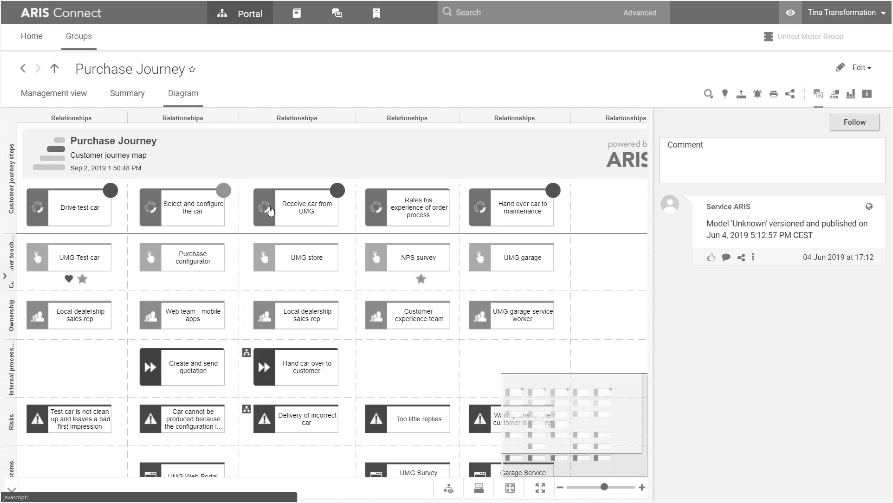
\includegraphics[scale=0.55]{DISSER-32.png}
    }
    \caption{Пользовательский интерфейс системы ARIS Platform}\label{fig:ARIS}
\end{figure}

\subsection{Инструмент системного анализа и проектирования StarUML}\label{sec:ch1/sec6/sub3}
Это программный инструмент визуального моделирования с открытым исходным кодом, который поддерживает стандартизованный язык графического описания UML для моделирования систем и программного обеспечения.
Программный продукт StarUML  от разработчика MKLabs предназначен для создания и применения графических моделей в нотации UML. Система основана на UML 2. 0 и предоставляет одинадцать различных видов диаграмм, активно поддерживая таким образом подход построения архитектур на базе моделей. Система может эффективно применяться системными аналитиками, проектировщиками и архитекторами систем, инженерами-программистами.
Программное обеспечение StarUML отличается высокой настраиваемостью в соответствии с пользовательской средой и высокой расширяемостью в своей функциональности. Использование StarUML обеспечивает высокую производительность и качество программных проектов.
Пользовательский интерфейс системы представлен на Рисунке ~\cref{fig:StarUML}.
\begin{figure}[ht1]
    \centerfloat{
        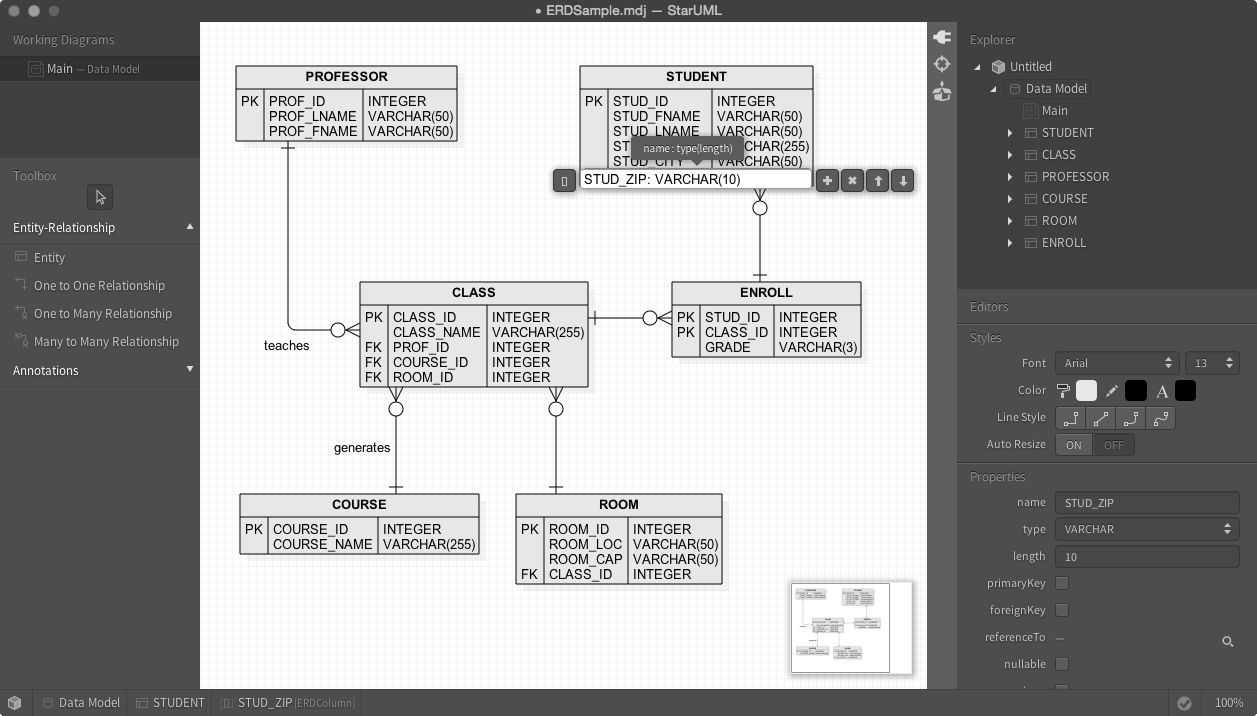
\includegraphics[scale=0.4]{DISSER-33.png}
    }
    \caption{Пользовательский интерфейс системы StarUML}\label{fig:StarUML}
\end{figure}

\subsection{Инструмент системного анализа и проектирования UNICOM System Architect}\label{sec:ch1/sec6/sub4}
Это комплексный программный инструмент бизнес и системного моделирования, позволяющий реализовывать в различных нотациях графические представления системы, требования к продукту и процесс проектирования и разработки программного обеспечения.
Программный продукт System Architect от компании-разработчика UNICOM прдназначен для визуального моделирования с целью снижения сложности предметной области и создаваемых систем, помогая более эффективно понимать сложные объекты и взаимодействовать в команде. Система UNICOM SA также помогает управлять рисками и соблюдением требований, одновременно повышая производительность и качество программных приложений и сервисов.
Пользовательский интерфейс системы представлен на Рисунке ~\cref{fig:UNICOM}.
\begin{figure}[ht1]
    \centerfloat{
        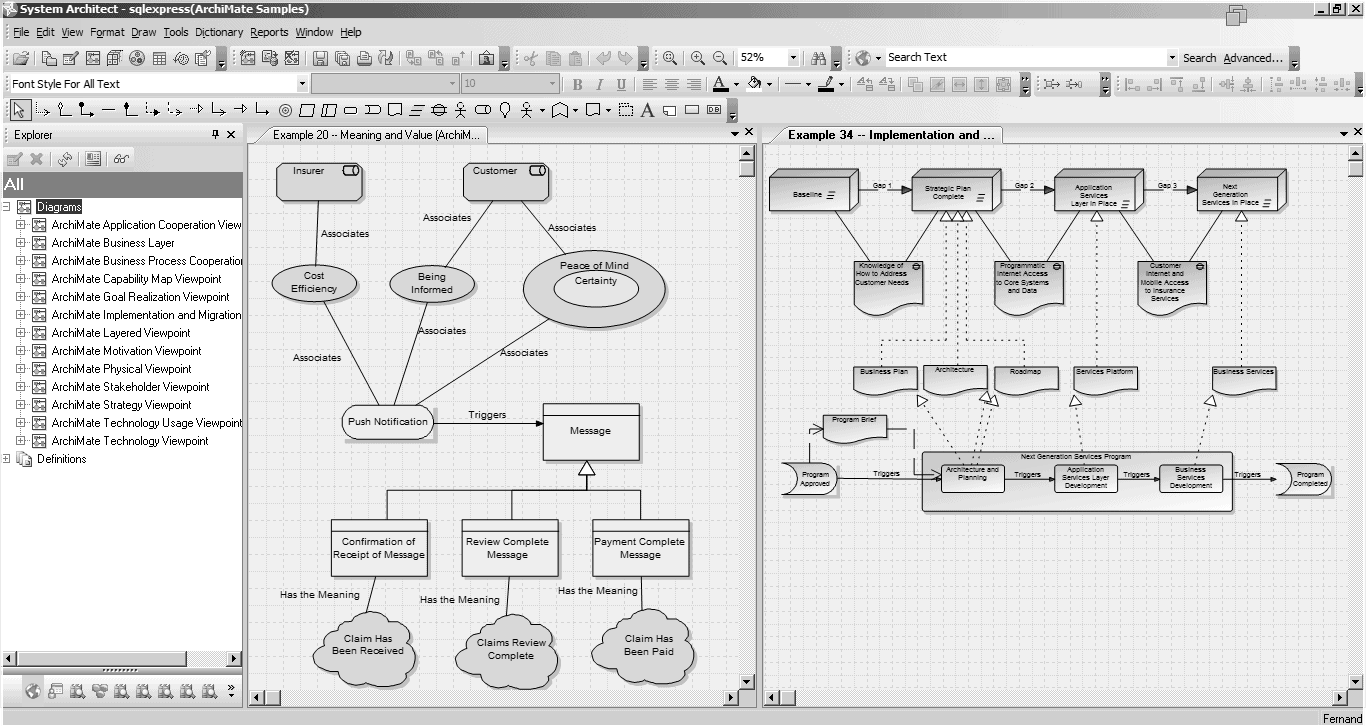
\includegraphics[scale=0.35]{DISSER-34.png}
    }
    \caption{Пользовательский интерфейс системы UNICOM System Architect}\label{fig:UNICOM}
\end{figure}

\subsection{Инструмент системного анализа и проектирования Microsoft Visio}\label{sec:ch1/sec6/sub5}
Инструменты Visio позволяют создавать диаграммы в один клик – перед этим достаточно внести все необходимые данные, и вы легко выполните нужную задачу. Программа позволяет предоставить информацию из готовой диаграммы – это делается с помощью формирования определенного отчета.
Приложение позволяет создавать чертежи, которые отличаются очень высоким уровнем информативности. Здесь используются различные элементы. Для каждой части чертежа составляются подробные комментарии.
Microsoft Visio позволяет выполнять масштабирование проекта. В качестве основы для построения схем могут использоваться системы для автоматического проектирования. Приложение предусматривает создание интерактивных панелей, которые могут использоваться для различных показателей.
Пользователи могут выполнять экспорт и импорт данных, который осуществляется между программами, входящими в пакет Office. Это увеличивает уровень удобства при работе с приложением. В программе также предусмотрена возможность для получения справки по работе с Visio. Здесь содержатся специальные подсказки и советы.
Пользовательский интерфейс системы представлен на Рисунке ~\cref{fig:Visio}.
\begin{figure}[ht1]
    \centerfloat{
        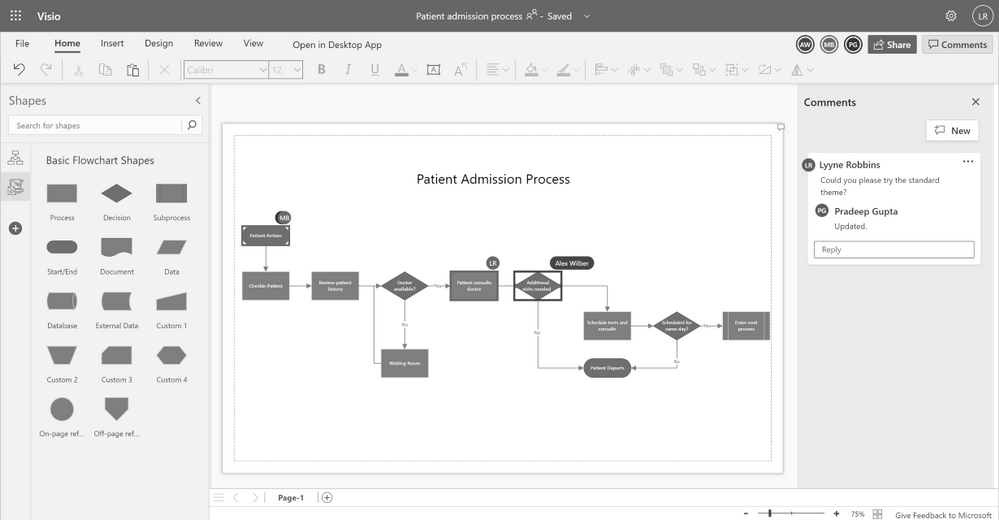
\includegraphics[scale=0.7]{DISSER-35.png}
    }
    \caption{Пользовательский интерфейс системы Microsoft Visio}\label{fig:Visio}
\end{figure}
\subsection{Инструмент системного анализа и проектирования Draw.io или Diagrams.net}\label{sec:ch1/sec6/sub6}
Это программа для управления требованиями, позволяющая предприятию любого размера создавать документы с требованиями, варианты использования и диаграммы. Программа позволяет создавать модели представления данных во всех нотациях, таких как, IDEF0, IDEF3, EPC, DFD, UML, ERD, PFDD. Существует, как облачная, так и standalone версии. Позволяет проектировать и рисовать схемы, диаграммы, бизнес-макеты, отношения между сущностями, программные блоки систем, а также элементы дизайна интерфейса программного обеспечения. В программе существует возможность добавлять палитру шаблонов для проектирования систем, согласно типам нотаций. Существует возможность экспортировать результаты работы в форматы: JPG, PNG, SVG, VDSX; программа поддерживает совместную работу: для экспорта чертежей сушествует формат .drawio, совместимый со всеми версиями программного продукта. Сервис поддерживает множество языков.
Пользовательский интерфейс системы представлен на Рисунке ~\cref{fig:Draw.io}.
\begin{figure}[ht1]
    \centerfloat{
        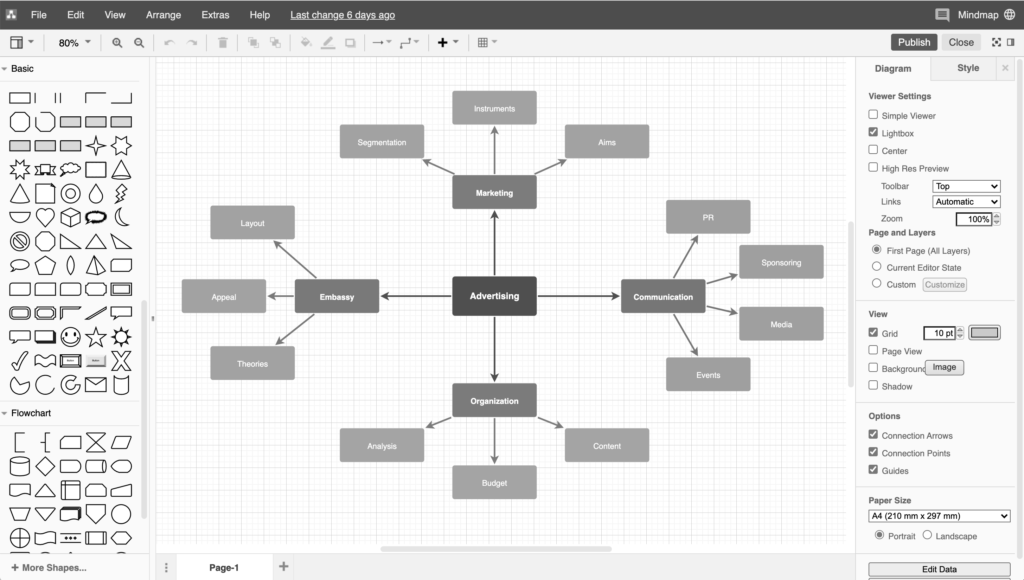
\includegraphics[scale=0.5]{DISSER-36.png}
    }
    \caption{Пользовательский интерфейс системы Draw.io или Diagrams.net}\label{fig:Draw.io}
\end{figure}

\subsection{Другие примеры}
Программ, которые помогают именно в проектировании архитектуры программного обеспечения на сегодняшний день на рынке не представлено. В основном, программы проектирования программного обеспечения предоставляют функционал по созданию: схем и чертежей в различных нотациях, графические представления системы, требования к продукту и процесс проектирования и разработки программного обеспечения. Таким образом, на данный момент явных аналогов системы не представлено.

\section{Выводы по главе}\label{sec:ch1/conc}
При проектированнии программного обеспечения среди профессиональных специалистов в этой области зачастую не хватает опыта для реализации оптимальной архитектуры программного обеспечения. Данный феномен может быть связан с различными факторами:  нехватки опыта, времени, кадров и т.д. Для того, чтобы узнать причины допущения ошибок при проектировании следует провести отдельное исследование, к данной работе этот вопрос не относится. В этой работе изучается вопрос построения системы поддержки принятия решений для проектирования архитектуры программного обеспечния. Автор работы не располагает сведениями и не изучает вопрос причин возникновения ошибок при проектировании программного обеспечения.
В данной главе был проведен обзор и систематизация основных проблем проектирования программного обеспечения. Была рассмотрена систе проектирования как полезная функция комбинации альтернатив инструментов реализации программного обеспечения. Рассмотрены наиболее распространенные инструменты проектирования программного обеспечния. Дано обоснование актуальности разработки систем поддержки принятия решений при проектировании архитектуры программного обеспечения.
\clearpage
           % Глава 1
\chapter{Разработка моделей и алгоритмов для проектирования архитектуры автоматизированной системы управления}\label{ch:ch2}
Автоматизированная система управления ставит перед собой цель повышение эффективности работы процессов автоматизации. В общем случае выделим следующие основные цели автоматизации процессов управления:
\begin{enumerate}
	\item предоставление информации для принятия решения, 
	\item ускорение выполнения технологических процессов и операций, 
	\item сбор, хранение и обработка данных необходимых для выполнения технологических процессов,
	\item повышение контроля и слежение за результатам производительности труда,
	\item повышение скорости принятия решений и стратегических процессов,
	\item оптимизация затрат и слежение за финансовыми ресурсами.
\end{enumerate} 

Условно информационные технологии предприятия можно разделить согласно Рисунку ~\cref{fig:ITclass} \cite{ITclass}.

\begin{figure}[ht1]
    \centerfloat{
        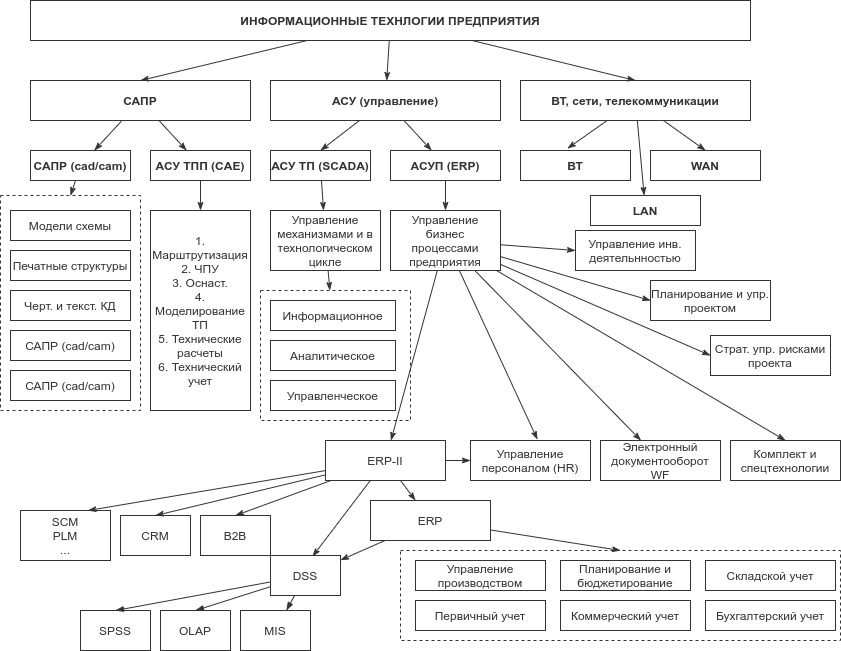
\includegraphics[scale=0.5]{DISSER-37.png}
    }
    \caption{Условная классификация информационных технологий предприятия}\label{fig:ITclass}
\end{figure}

Принципы проектирования программного обеспечения должны укладываться в следующие критерии, указанные на Рисунке~\cref{fig:principles}.  

\begin{figure}[ht]
    \centerfloat{
        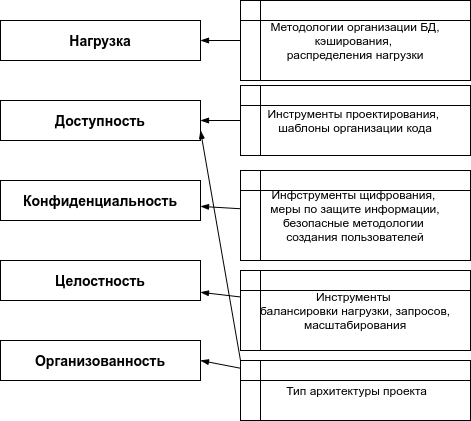
\includegraphics[scale = 0.8]{Dissertation/images/DISSER-52.png}
    }
    \caption{Принципы проектирования архитектуры программного обеспечения}\label{fig:principles}
\end{figure}

Автоматизированные системы управления, как понятие, появилось в СССР в 60-х годах двадцатого века в связи с внедрением вычислительной техники в организацию руководства СССР \cite[с.~38]{Yakovenko}. Для управления предприятием требуется контролировать все процессы, происходящие на предприятии, т.к. в зависимости от успешного ведения дел предприятия зависит его эффективность. Во многом кортролировать эффективность работы предприятия помогает внедрение автоматизированной системы управления, т.к. такая система позволяет следить за выполнением тех или иных процессов работы предприятия. Типовая автоматизация процессов предприятия включает в себя следующие направления:

\begin{enumerate}
	\item автоматизация процессов деятельности предприятия (например, бухгалтерский учет, управление персоналом, логистика, управление снабжением и т.д.),
	\item автоматизация основных технологических процессов предприятия,
	\item автоматизация процессов управления, процессов принятия решения, анализа, стратегического планирования деятельности предприятия.
\end{enumerate}

В целом, все предпрития условно можно разделить на 2 класса:
\begin{enumerate}
	\item предприятия с дискретным типом производства,
	\item предприятия с непрерывным производством.
\end{enumerate}

Единое информационное пространство предприятия состоит из совокупности всех баз, информационных банков данных, информационных технологий, информационно-вычислительных систем, телекоммуникационных сетей, протоколов безопасности, которые составляют единое информационное пространство для взаимодействия тех или иных субъектов технологического производства.

Единое информационное пространство условно можно представить согласно Рисунку ~\cref{fig:ITspace}.

\begin{figure}[ht1]
    \centerfloat{
       
       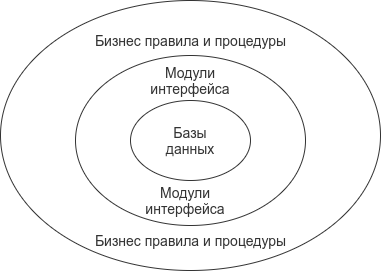
\includegraphics[scale=0.50]{DISSER-38.png}
    }
    \caption{Условная классификация информационных технологий предприятия}\label{fig:ITspace}
\end{figure}
Таким  образом, информационные технологии предприятия собирают в себе комплекс программно-аппаратных информационных средств составляющих интегрированную информационную среду: комплекс программно-ориентированных взаимосвязанных информационных подсистем, разрабатываемых для единого информационного пространства предприятия.

Интегрированная информационная среда, как единое информационное пространство предприятия представляется в следующем обобщенном виде, как на Рисунке ~\cref{fig:ITembeddedspace} \cite{ITclass}.

\begin{figure}[ht1]
    \centerfloat{
        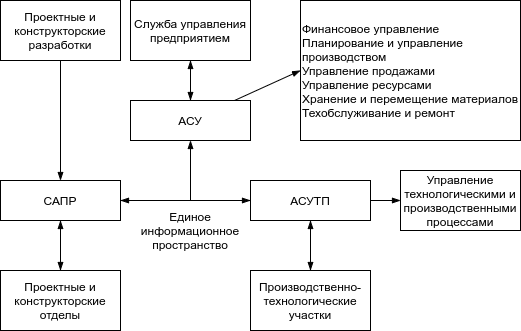
\includegraphics[scale=0.8]{DISSER-39.png}
    }
    \caption{Концептуальная модель интегрированной информационной среды}\label{fig:ITembeddedspace}
\end{figure}

Следующие компоненты составляют типовую интегрированную информационную среду:
\begin{enumerate}
	\item телекоммуникационная среда в составе коммуникационного программного обеспечения,
	\item средства организации коллективной работы сотрудников,
	\item информационные ресурсы (ERP системы, программное обеспечение управления документооборотом, информационая поддержка предметных областей, программное обеспечение анализа информации и поддержки принятия решения, программное обеспечение управления проектами),
	\item инфраструктура для организации информационной среды,
	\item система обучения персонала, система переподготовки кадрового персонала.
\end{enumerate}
Систематизируем общие типовые требования для проектированая интегрированной информационной среды предприятия:
\begin{enumerate}
	\item интеграция горизонтальная и вертикальная существующего программного обеспечения с новым функционалом,
	\item единство организационных, технических и технологических принципов построения информационной среды,
	\item единая парадигма обмена информации и передачи данных на основе различных физических носителях,
	\item соответствие международным и российским стандартам разработки программного обеспечения,
	\item обспечение доступа пользователей к базам данных и необходимым источникам информации,
	\item обеспечение информационной безопасности и многоуровневой защиты данных, обеспечение гарантии подлинности информации,
	\item средства коллективного доступа к информационной среде,
	\item применение принципа модульности при проектировании системы и ее состовляющих подсистем,
	\item внедрение сертифицированных решений и решений, соответсвующих стандартам,
	\item мониторинг инфорационных средств и решений,
	\item использование методологий для совершенствования внедренных технологий.
\end{enumerate}
Таким образом, при проектировании информационной среды требуется следующий аналитический базис для планирования работ: 
\begin{enumerate}
	\item реалистичная оценка действительности для планирования взаимодействия с информационной средой всех пользователей системы,
	\item единый центр принятия решений при планировании работ для согласованной работы всех субъектов взаимодействия информационной среды во избежании несогласованных с имеющимися в пользовании средств и инструментов информационной среды,
	\item полезный результат, получаемый от организации информации, информационной среды, информационного пространства,
	\item анализ лучших практик организации информационной среды, информационного пространства, внедренных на рынке,
	\item понимание целей информатизации конкретного объекта информатизации, понимание полезного результата с внедрения информатизации для объекта,
	\item транслирование внедренных технологий во внешних мир для развития рынка в этой области.
\end{enumerate}

Экспертная система на основе искусственного интеллекта, которая обрабатывает слабоструктурированную и трудно формализуемую информацию в некоторой предметной области, может интерпретировать и объяснять методы решения задач принятия решения. Экспертные системы способны анализировать и предлагать множество решений на основе некоторых параметрических критериев. Такие системы обрабатывают информацию на основе некоторых формализованных структуированных закономерностях логического вывода, в данной работе модулем выявления закономерностей выступает критерий максимума взвешенной информативности.

Элементами экспертной системы являются следующие модули блоки обработчики:
\begin{enumerate}
    \item база знаний — некоторое семантическое представление знаний, формализованных в виде базы закономерностей, построенной на основе отбора критерием максимума взвешенной инфрмативности по таблице каналов наблюдений на основе ТРИЗ методологии,
    \item блок логического выводе — блок, который моделирует механизм поиска закономерностей, на основе отбора каналов наблюдения и классификации на основе критерия максимума взвешенной информативности,
    \item блок интерпретаций — блок, который интерпретирует некоторое семантическое представление получаемых системой данных,
    \item блок формирования рекомендаций — данный блок формирует рекомендации.
\end{enumerate}

Таким образом, системы поддержки принятия решения, основанные на экспертных системах, главным образом, опираются на модуль формирования закономерностей.

\section{Классы автоматизированных систем управления}\label{sec:ch2/sec1}
Классы автоматизированных систем управления:
\begin{enumerate}
	\item ОГАС - общегосударственная автоматизированная система сбора, хранения и обработки данных для задач учета, планирования и управления народным хозяйством страны в целом,
	\item ОАСУ — отраслевая автоматизированная система управления, объектом которой является определенная отрасль народного хозяйства страны;
	\item АСУП — автоматизированная система управления предприятием на основе применения вычислительных систем и экономико-математических методов для решения основных задач производственно-хозяйственной деятельности. Цель АСУП заключается в обеспечении неуклонного увеличения выпуска продукции путем непрерывного повышения технического и организационного уровня производства;
	\item АСУТП — автоматизированная система управления технологическим процессом, предназначенная для выработки и реализации управляющих воздействий на технологический объект управления (ТОУ) в соответствии с принятым критерием оптимальности..
\end{enumerate}
Рассмотрим внимательнее информационные потоки и процессы, которые отображают деятельность объекта автоматизации для:
\begin{enumerate}
	\item автоматизированных систем управления предприятием,
	\item автоматизированных систем управления технологическим процессом.
\end{enumerate}

Автоматизированная система управления состоит из множества подсистем, в основном они раздеделяются на две модели:
\begin{enumerate}
	\item нормативная модель управления,
	\item модель управления текущими состояниями.
\end{enumerate}

Нормативная модель управления представляет собой модель планирования ресурсов для обеспечения работы процессов на производстве:
\begin{enumerate}
	\item коэффициенты расчета показателей использования материально-технических средств,
	\item коэффициенты расчета показателей использования энергетических ресурсов,
	\item коэффициенты расчета показателей трудоемкости использования деталей,
	\item коэффициенты расчета показателей произвоительности труда,
	\item коэффициенты расчета показателей использования финансовых фондов,
	\item коэффициенты расчета показателей экономической эффективности.
\end{enumerate}

Модель текущих состояний расчитывается на основе текущей информации, получаемой в результате выполнения функции учета текущих состояний и планируемыми показателями.

Таким образом, для принятия решений расчитывается дифференциал между текущей информацией, получаемой в результате выполнения функции учета текущих состояний и планируемыми показателями.

Автоматизированные системы управления предприятием состоит из двух основопологающих подсистем:
\begin{enumerate}
	\item управляемая подсистема,
	\item управляющая подсистема.
\end{enumerate}
Управляемая подсистема является объектом, а управляющая подсистема является субъектом. В управлемой системе главными объектами иныформатизации выступают материальные и энергетические потоки. В управляющей системе главными объектами выступают информационные процессы и потоки.

В автоматизированных системах управления предприятием основной целью работы системы является предоставление информации для принятия решений в управлении предприятием. В автоматизированных системах управления технологическим процессом основной целью является контроль за выполнением технологического процесса.

Функциональные подсистемы АСУП можно разделить на следующие категории :
\begin{enumerate}
	\item управление технической подготовкой процессов производства,
	\item планирование экономических и технических производств,
	\item оперативное управление процессами основного производства,
	\item управление материальными ресурсами,
	\item управление бухгалтерской и финансовой документации,
	\item управление кадровым персоналом,
\end{enumerate}
Управляющая подсистема управляет соответвующим объектом: функциональной подсистемой.
Автоматизирования подсистема технико-экономического планирования создается для прогнозирования развития производства:
в своем составе типовая подсистема решает следующие задачи:
\begin{enumerate}
	\item расчет оперативных планов-графиков, регламентирующих выпуск продукции в соответствии с материальными, техническими, экономическими и производственными возможностями, 
	\item определение возможностей наращивания производства согласно оценке темпов расширения производства,
	\item расчет и формирование планов выпуска продукции.
\end{enumerate}
Уровень детализации прогнозов определяется периодом прогнозирования. Существуют следующие виды типовых прогнозов в подсистемах технико-экономического планирования :
\begin{enumerate}
	\item производственно-стратегический прогноз,
	\item планирование выпуска на относительно большие промежутки времени,
	\item прогнозы производственного цикла.
\end{enumerate} 
Целью подсистемы технико-экономического планирования:
\begin{enumerate}
	\item определение основных напрвлений развития производства,
	\item определение объемов, сроков, ресурсов и т.д. для слежением за показателями производства,
	\item определение потребности в трудовых, метариеальных и финансовых ресурсов,
	\item определение результатов производственно - хозяйственной деятельности производства.
\end{enumerate}
Автоматизированая система управление технологическими процессами создается для организации технологической подготовки производства. Процессы технологической подготовки производства представляют собой следующее: это некоторое множество мероприятий, которые отвечают за технологическую подготовки производства, необходимых для выпуска заданного плана производства.
Основные функции технологической подготовки производства:
\begin{enumerate}
	\item разработка технологических процессов,
	\item проектирование и изготовление средств технического и технологического производства,
	\item организация процессов технологического производства.
\end{enumerate}
Основными задачами системы являются:
\begin{enumerate}
	\item предоставление информационных ресурсов для организации освоения производства новых изделий существующего образца,
	\item предоставление информационных ресурсов для организации создания новых изделий.
\end{enumerate}
Типовые процессы в автоматизированных системах управления технологическими процессами являются:
\begin{enumerate}
	\item измерение параметров технологического производства,
	\item измерение темпов технологического производства,
	\item измерение девиантности и отклонений от параметров производства,
	\item измерение процессов согласно командам оператора.
\end{enumerate}
Функции, которые подвергаются автоматизации:
\begin{enumerate}
	\item определение режимов технологического производства,
	\item формирование управляющих воздействий режимов технологического производства,
	\item управление математической моделью и параметрами технологического производства,
	\item регистрация технологических и экономических показателей технологического производства,
	\item распределение материальных, энергетических, кадровых потоков для задач обеспечения необходимого режима технологического производства,
	\item распределение ремонтных мероприятий между технологическим производством,
	\item распределение учебных мероприятий технологического производства,
	\item распределение плановых графиков и сменно-суточных работы для технологического производства.
\end{enumerate}
АСУТП различает в среднем пять видов режимов работы:
\begin{enumerate}
	\item режим сбора и обработки информации,
	\item рекомендательный режим,
	\item режим контроля и управления,
	\item режим непосредственного управления посредством цифрового манипулятора,
	\item иерархические системы управления.
\end{enumerate}

Режим сбора и обработки данных состоит из отчетов аналитической информации, которая поступает после сбора и обработки данных с технологического производства. Такие измерения могут проводится посредством системы датчиков, измерителей, специальных приборов, которые имеют способность собирать информацию с технологического производства и его процессов. Главной задачей данного режима является предоствление отчетов  в виде аналитической информации. Все результаты зачастую сохраняются в реестр или спецальный архив.
Режим рекомендательный главной задачей ставит формирование рекомендаций по:
\begin{enumerate}
	\item выбору подходящего режима работы технологического производства при заданных параметрах,
	\item определению управлеющих воздействий по переменным возделйствия на процесс технологического производства,
	\item определение локальных регуляторов процессов технологического производства.
\end{enumerate}
Режим контроля и управления состоит, в общем случае, из двух уровневой иерархической модели:
\begin{enumerate}
	\item нижнгий уровень отвечает за управление локальными регуляторами процессов технологического производства,
	\item верхний уровень отвечает за контроль параметров состония технологического процесса посредством сбора информации с датчиков контроля параметров.
\end{enumerate}

Режим непосредственного управления посредством цифрового манипулятора отвечает за формирование управляющих воздейством через ЭВМ, соединенную непосредственно с управляемым объектом.
Иерархические системы управления - система, состоящая из множества уровней подсистем, находящихся в соподчинении.
Первый уровень представляет собой подсистему, которая непосредственным образом управляет технологическим процессом или технологическими операциями.
Второй уровень представляет собой подсистему, которая осуществляет расчет и оперативную корректировку режимов технологических операций или процессов.
Третий уровень представляет собой центральную управляющую подсистему, которая осуществляет расчет, корректировку технологического режима всего процесса в целом.

Каждая подсистема имеет соответствующую ей ЭВМ, которая работает в одном из четырех описанных выше режимов.

\subsection{Типы транзакционных систем}\label{sec:ch2/sec1/sub1}

Система должна обладать следующими свойствами:
\begin{enumerate}
	\item сложность,
	\item делимость,
	\item целостность,
	\item многообразие элементов системы и различие их природы,
	\item структурность,
	\item адаптивность,
	\item интегрируемость. 
\end{enumerate}
Системы можно классифицировать согласно типам транзакций, которые происходят в системе.
Информационные потоки в транзакционных системах чаще всего классифицируются по типу хранения и обработки информационного потока данных. Классифицируем данные по следующим признакам:
\begin{enumerate}
	\item данные по деталям, чаще всего обработка элементарных данных,
	\item агрегированные данные, чаще всего суммирование по некоторым измерениям,
	\item метаданные, т.е. данные, которые могут описывать некоторые конфигурационные действия над данными (обстоятельства использвания данных).
\end{enumerate}
Данные образуют некоторый информационный поток, который может быть разделен по следующим направлениям:
\begin{enumerate}
	\item входной поток,получаемый системой при обработке (источником информации может служить любой объект),
	\item потоки сообщений, которые образуются в результате работы деловой логики взаимодействия объектов,
	\item архивные потоки, образуются из классов данных, спрос на выполнение которых стал устаревать,
	\item поток метаданных, данные, которые образовались за счет конфигурационных, логгированных, журналированных даннных,
	\item выходной поток, данные, которые получает пользователь на выходе из работы системы,
	\item обратный поток, данные, которые возвращаются в систему.
\end{enumerate}

\subsection{OLTP системы}\label{sec:ch2/sec1/sub2}
OLTP  транзакционная система - система обработки транзакций в реальном времени. Такие системы предназначены для ввода, обработки и структурирования информации в режиме реального времени. К таким системам обычно предъявляются следующие требования:
\begin{enumerate}
 	\item ограничения на обработку информации через реальное время, 
 	\item транзакционные модели данных должны быть сильно нормализованы,
 	\item в случае возникновения ошибок, транзакции должны возвращаться в исходное состояние, до момента начала совершения транзакции,
 \end{enumerate}
Компоненты исполнения транзакций являются частью компонентов нагрузки, исполнение которых ограничиваются строгими требованиями выполнения в определенный интервал времени. Более того, транзакции, после отработки постоянно обновляют базу данных. Для проектировании подобных систем следует учитывать следующие параметры и характеристики работы программного обеспечения:
\begin{enumerate}
	\item при проведении транзакции используется относительно небольшой объем данных,
	\item индексы в базу данных должны быть легко доступны для уменьшения времени обработки транзакции,
	\item система должна иметь относительно небольшой промежуток временного отклика,
	\item используются только нормализованные формы транзакционные модели,
	\item может поддерживать сложные транзакционные модели,
	\item модель обработки транзакций проектируется опираясь на требования по нижнему пределу ограничения пропускной способности информации.
\end{enumerate}
Таким образом, основная цель OLTP систем - предоставление доступа в ограниченном отрезке реального времени, в строгом соответствии с нижним пределом пропускной способности. Суть таких систем состоит в соблюдении ограничений по обработке транзакций в строго определенном режиме обработки: ограниченного во времени, ограниченного в нижнем пределе по нагрузке. Система должна обеспечивать вычислительную нагрузку в реальном времени в стогом соответствии с ограничениями по времени и пропускной способности. Система должна восстанавливаться  в исходное состояние транзакций в случае выявления ошибок обработки. Система должна обновлять значения базы данных после проведения каждой успешной транзакции. В системе основным критерием успешной работы является обработка транзакции за ограниченный период в реальном времени. Такие системы не ориентированы на сохранение данных, при надобности данные системы архивируются.

\subsection{OLAP системы}\label{sec:ch2/sec1/sub3}

OLAP системы - это системы, которые ориентированы на аналитическую обработку данных. Такие системы анализируют данные многомерные данные и чаще всего используются для построения анализа многомерных систем.

Цель таких систем, предоставление аналитических отчетов, поэтому фундаментом обработки данных становится база данных, основанная на фактах. Таблица фактов - является сердцем таких систем, правильно спроектированная таблица фактов, которых соблюдаются все правильно низкой связности и высокой группировки, обеспечивает быстрое время обработки запросов в таких системах. 

Таблица фактов содержит фактическую информацию о свойстве объектов или событий. Факты делятся по следующим признакам:
\begin{enumerate}
	\item факты о транзакциях, т.е. факты, хранящие информацию о конретных совершенных действиях, 
	\item факты о состояниях,
	\item факты о свойствах того или иного объекта,
	\item факты о событиях.
\end{enumerate}

Таблица фактов должна содержать один внешний составной ключ, который должен объединять первичные ключи таблиц измерений. В настощее время разработано множество стандартов для проектирования OLAP систем. В общем случае, архитектура таких систем относится к обработке анализа, хранения и преобразования данных в независимых слоях системы, абстрактно ограниченных программным кодом. Основная нагрузка в таких системах ложится на организацию составления аналитических данных, где могут применяться различными методы решения вывода и аггрегации инфомации: например, путем изоляции обращений к базе данных, через объектно реляционные запросы на высокоуровневом языке программирования, либо оптимизация запросов к базе данных. 
Подходы к проектированию систем будут рассмотрены более подробно далее в работе.

\subsection{Блокчейн системы}\label{sec:ch2/sec1/sub4}

Модель транзакций в блокчейн системах представляется собой линейно независимую модель распределенных транзакций и может быть задана в следующем виде, где $y_i, i=1,2, …, N$ отображает транзакции, проводимые за некоторый конечный промежуток времени :
\begin{equation}
	\begin{cases}
		y'_{1}= a_{11}(x)y_{1}+a_{12}(x)y_{1}+ ... + a_{1n}(x)y_{n}, \\
		y'_{2}= a_{21}(x)y_{1}+a_{22}(x)y_{1}+ ... + a_{2m}(x)y_{n} , \\
		... \\
		y'_{n}= a_{n1}(x)y_{1}+a_{n2}(x)y_{2}+ ... + a_{nm}(x)y_{n}. 
	\end{cases}
\end{equation}



В матричной форме эта система имеет вид $\bar{y'}(x)=A(x)y(x)$, где $A(x)$ – квадратная функциональная матрица коэффициентов 
$\bar{y}=(y_1(x),  y_2(x), …,y_n(x))^T$ – функциональный вектор—столбец неизвестных, $\bar{y'}=(y'_1(x),  y'2(x), ... ,y'_n(x))^T$ – функциональный вектор—столбец производных неизвестных системы уравнений.

Так как элементы матрицы $A$ являются постоянными функциями непрерывные на любом промежутке, то по теореме о структуре общего решения линейной однородной системы дифференциальных уравнений для того, чтобы найти общее решение $y_0= C_1\bar{y}_1(x)+C_{2}\bar{y}_{2}(x)+ ... + C_{n}\bar{y}_{n}(x)$ данной системы уравнений достаточно построить фундаментальную систему решений $\bar{y}_{1}(x), \bar{y}_2(x), ... , \bar{y}_n(x)$.

Как было предложено Л. Эйлером, будем искать решение $y(x)= \bar{g}e^{kx}$ т.е. линейную однородную систему дифференциальных уравнений с постоянными коэффициентами в виде произведения $n$ — мерного вектора $\bar{g} \neq 0$  на экспоненциальную функцию $e^{kx}$, где $k$  – некоторое число. Дифференцируя эту вектор—функцию и подставляя полученные функции в решаемое дифференциальное уравнение, получим $\bar{g}ke^{kx}=A\bar{g}e^{kx}$. 

Так как экспоненциальная функция строго положительна, то справедливо матричное уравнение $(A-kE)\bar{g}= 0$, которое позволяет найти собственные числа и собственные векторы матрицы коэффициентов $A$.Одним из методов вычисления собственных чисел матриц является решение уравнения $\bigtriangledown(A-kE) = 0$, которое следует из теоремы существования ненулевого решения линейной однородной алгебраической системы уравнений. Раскрывая определитель, получаем алгебраическое уравнение $k^n+ p_{n-1}k^{n-1}+p_{n-2}k^{n-2}+ ...+ p_0=0$   порядка $n$  относительно переменной $k$. В теории дифференциальных уравнений данное уравнение называют \textit{характеристическим уравнением} линейная однородная система дифференциальных уравнений. Для каждого собственного числа $k_i$  из матричного уравнения $(A-k_{i}E)\bar{g}=0$  находят некоторый собственный вектор $\bar{g}_i\neq0$. По построению вектор—функция $\bar{y}_i(x)= \bar{g}_{i}e^{k_{i}x}$  является одним из решений исходного линейной однородной системы дифференциальных уравнений.

Требования к блокчейн приложениям обобщены на Рисунке~\cref{fig:blockchhainreq}. Типовые архитектурные элементы  


\begin{figure}[ht]
    \centerfloat{
        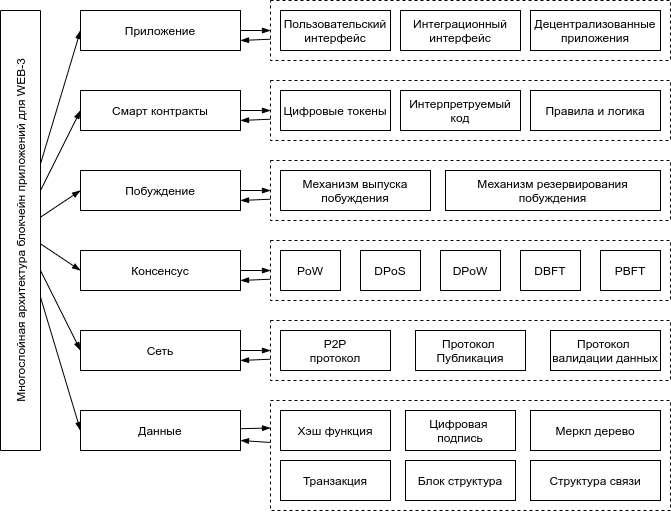
\includegraphics[scale=0.6]{Dissertation/images/DISSER-54.png}
    }
    \caption{Обобщенная архитектура в блокчейн приложениях согласно Индустрии 4.0}\label{fig:blockchhain}
\end{figure}

\begin{figure}[ht]
    \centerfloat{
        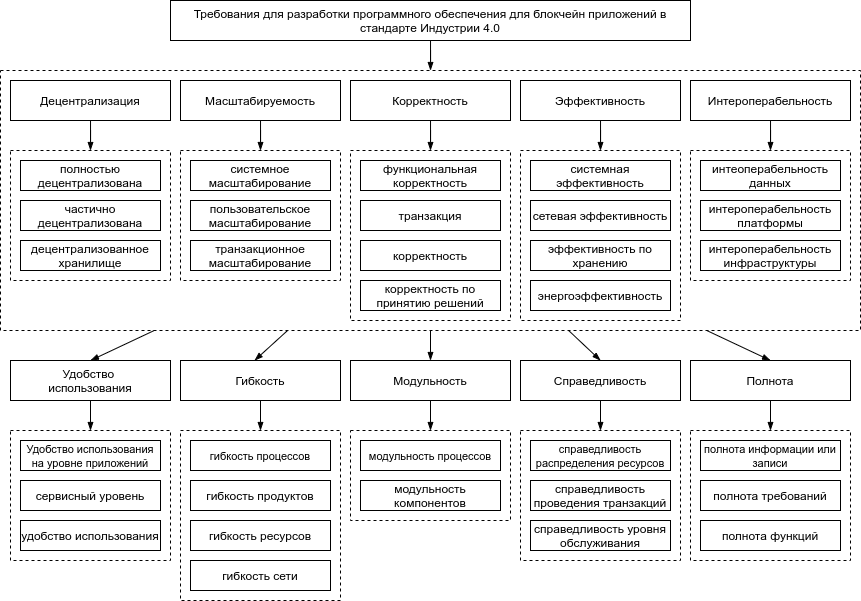
\includegraphics[scale=0.5]{Dissertation/images/DISSER-55.png}
    }
    \caption{Требования к блокчейн приложениям}\label{fig:blockchhainreq}
\end{figure}

\subsection{Высоковычислительные системы}\label{sec:ch2/sec1/sub5}


\subsection{Высоконагруженные системы}\label{sec:ch2/sec1/sub6}


\subsection{Типы предоставления доступа}\label{sec:ch2/sec1/sub7}

Системы автоматизированного управления могут быть разделены по следующим моделям предоставления доступа:
\begin{enumerate}
	\item SaaS модель предоставления доступа,
	\item PaaS модель предоставления доступа,
	\item IaaS модель предоставления доступа.
\end{enumerate}

\subsection{SaaS системы}\label{sec:ch2/sec1/sub8} 

SaaS система - система организации кода в виде предоставления доступа к программному обеспечению, как к услуги. 
Программное обеспечение системы SaaS обладает следующими ключевыми признаками:
\begin{enumerate}
    \item доступ к программному обеспечению, разработанному в соответствии с моделью программного обеспечения, как услуга, предоставляется удалённо по сетевым каналам и, как правило, через веб-интерфейс, кроме того, могут использоваться тонкие клиенты и терминальный доступ;
    \item программное обеспечение развёртывается в центре обработки данных в виде единого программного ядра, с которым работают все заказчики;
    \item обслуживание и обновление программного обеспечения выполняется централизованно на стороне поставщика приложения, предоставляемого как услуга (SaaS).
\end{enumerate}

\subsection{PaaS системы}\label{sec:ch2/sec1/sub9}
PaaS система предоставляет доступ к программному обеспечению через платформу. Платформа, предоставляется, как услуга. Чаще всего модель предоставляется, как облачный сервер с набором реализованного функционала или инструментария в аренду под конкретные цели. Модель, предоставляется за счет облачных вычислений, реализованных на облачном сервере. Функционал информационно-вычислительной инфраструктуры, включая вычислительные серверы, серверы, системы хранения, целиком управляется провайдером услуг. 


\subsection{IaaS системы}\label{sec:ch2/sec1/sub10}
IaaS системы - это такой тип систем, который предоставляет инфроструктуру как сервис. Чаще всего данные размещаются на облаке или в гибридном доступе, функционал по разработке инфраструктуры предоставляется по подписке. С помощью модели IaaS инфраструктура располагается на облаке, как набор сервисов.
С помощью модели IaaS компании могут частично или полностью переместить в облако локальную инфраструктуру центра обработки данных, где ее обслуживанием и управлением занимается поставщик облачных сервисов. К числу таких экономически эффективных элементов инфраструктуры могут относиться вычислительные и сетевые ресурсы, оборудование для хранения данных, а также другие компоненты и программное обеспечение. 
В рамках стандартной модели IaaS компании любого размера используют различные сервисы, такие как вычислительные ресурсы, хранилище и базы данных, предоставляемые поставщиком облачных решений. Поставщик услуг предоставляет эти сервисы путем размещения оборудования и программного обеспечения в облаке. Компании при этом не требуется приобретать собственное оборудование, заниматься его администрированием и отводить под него место в своих центрах обработки данных. А затраты она несет по модели «оплата по мере использования». Если компании нужно меньше ресурсов, общие затраты на них снижаются. А по мере роста компания может за считаные минуты предоставить сотрудникам дополнительные вычислительные ресурсы и другие технологии.
\section{Постановка задачи проектирования архитектуры автоматизированных систем управления, основные ограничения и допущения}\label{sec:ch2/sec2}

При проектировании системы основопологающими принципами проектирования является соблюдение следующих стратегий:
\begin{enumerate}
	\item миссия и видение проекта,
	\item руководящие принципы,
	\item цели, задачи, стратегии,
	\item архитектура ИТ.
\end{enumerate}

Соблюдение следующих тактик:
\begin{enumerate}
	\item политики и правила,
	\item ИТ - стандарты,
	\item Процедуры,
	\item Руководства.
\end{enumerate}

Изобразим данную парадигму проектирования в следующем виде, согласно Рисунку~\cref{fig:StrategyM}.
\begin{figure}[ht1]
    \centerfloat{
        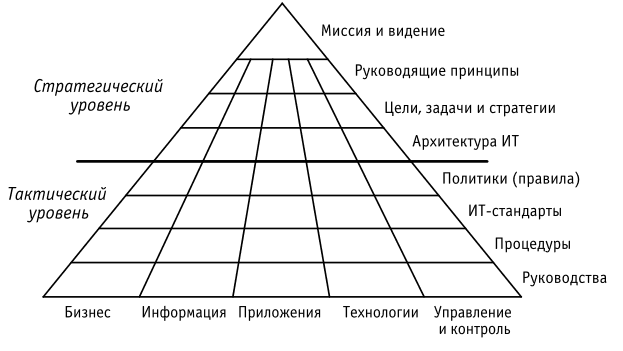
\includegraphics[scale=0.7]{DISSER-40.png}
    }
    \caption{Основопологающие принципы проектирования}\label{fig:StrategyM}
\end{figure}

Данный рисунок показывает, что руководящие принципы при проектировании системы накладывают ограничения на конкретные принципы, тактики и стратегии. Перейдем к рассмотрению ТРИЗ в разделе 2.3.1 подробнее далее. Но сейчас остановимся на более подроьном рассмотрении приципов проектирования архитектуры. 
\subsection{Принципы проектирования}\label{sec:ch2/sec1/sub11}
 Самыми главными элементами описания информационной архитектуры проектирования ИТ системы являются следующие:
 \begin{enumerate}
 	\item Миссия и видение.
 	\item Руководящие принципы.
 	\item Цели, задачи и стратегии.
 	\item Архитектура информационной технологии.
 	\item Политики и правила.
 	\item ИТ - стандарты.
 	\item Процедуры.
 	\item Руководства и рекомендации (best practices).
\end{enumerate}

Существует два основных направления проектирования архитектуры : 
\begin{enumerate}
	\item на основе принципов,
	\item на основе моделей.
\end{enumerate}

В архитектурной методике, разработанной Togaf\cite{Togaf}, эти два напрваления комбинирует в следующий принцип: придерживаться деклараций и следованию принципов, описывая состояния архитектуры в виде моделей, описывающие отдельные домены представлений.
Согласно представлению NASCIO (Национальная ассоциация руководителей информационных служб штатов США), влияние различных компонентов друг на друга представимо в следующем виде на Рисунке~\cref{fig:NASCIO}.
\begin{figure}[ht1]
    \centerfloat{
        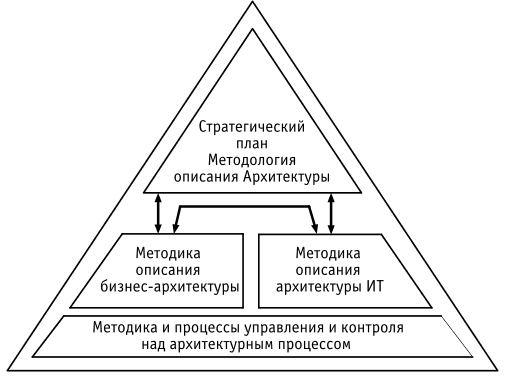
\includegraphics[scale=0.7]{DISSER-41.png}
    }
    \caption{Влияние различных компонентов друг на друга согласно модели NASCIO}\label{fig:NASCIO}
\end{figure}

Таким образом, архитектура представляет собой целостный процесс, который основан на ключевых стратегиях. Ключевые стратегии в свою очередь связывают бизнес, организацию, производство, информацию, прикладные системы, технологические процессы.
Интересным определением архитектуры является выражение Билла Гейтса в его книге "Бизнес со скоростью мысли", в которой он сравнивает архитектуру с электроной нервной системой предприятия. В его понимании, архитектура, подобно нервной системе, есть совокупность электронных процессов, которая должна адекватно воспринимать мир и реагировать на изменения, происходящие в нем.  

Архитектура программного обеспечения автоматизированной информационной системы представляет собой взаимосвязанную систему компонентов и модулей, которые стремятся обеспечить решение некоторой поставленной задачи автоматизации. Архитектура состоит из множества технических решений, которые можно комбинировать некоторым способом, архитектура допускает множество технических реализаций путем выбора различных компонентов архитектуры и методов взаимодействия между ними. В данной работе представлена модель архитектуры т.е. модель Библиотекаря для проектирования высоконагруженных автоматизированных информационных систем, с выполнением необходимых свойств, описанных выше.  
Перечислим типовой перечень сервисов и служб, необходимых для проектирования автоматизированной информационной системы:
\begin{enumerate}
	\item организация хранилища данных;
	\item организация обработки данных;
	\item формирование деловых функций объекта автоматизации;
	\item создание пользовательского интерфейса;
	\item разработка каналов обмена и передачи информации для интеграции со сторонними сервисами или ресурсами.
\end{enumerate}
Основополагаюшими понятиями в проектировании архитектуры для автоматизированной системы управления являются следующие объекты:
\begin{enumerate}
	\item ресурсы проектируемой информационной системы,
	\item процессы проектирумой информационной системы,
	\item состояния процессов проектируемой информационной системы,
	\item производительность процесса проектируемой информационной системы,
	\item информационная нагрузка на процесс проектируемой информационной системы,
	\item информационный поток на процесс проектируемой информационной системы,
	\item информационный объем на процесс проектируемой информационной системы,
	\item риск потери информации в процессах проектируемой информационной системы,
	\item производительность информационной системы в целом.
\end{enumerate}
Не менее важным вопросом при проектировании информационной системы является определение \textbf{объектов, которые будут структурировать данные}.


Процессы в информационной системе охарактеризуем, как следующие виды действий в типовой информационной системе на обобщенном уровне:
\begin{enumerate}
    \item действие введения информации из внутреннего ресурса,
    \item действие введения информации из внешнего ресурса,
    \item действие обработки информации во внутреннем ресурсе,
    \item действие обработки информации во внешнем ресурсе,
    \item действие по хранению информации во внутреннем ресурсе,
    \item действие по хранению информации во внешнем ресурсе,
    \item действие по передаче информации во внутренний ресурс,
    \item действие по передаче информации во внешний ресурс.
\end{enumerate}


Впоследствие, при проектировании информационной системы, действия в конкретной деловой логике можно категоризировать согласно видам действий, описанным выше.

Формализуем данную задачу. 

Пусть множество типов информационных систем, описываемых пользователем как  $U=\{u1,u2,...,un\}$, множество объектов, т.е. предлагаемых архитектур $P=\{p1,p2,...,pm\}$, весовая матрица  $R=ri,j$ размера $nxm$,  $i\{1...n\},j\{1...m\}$. $N$ - желаемое количество рекомендаций, которые нужно получить от системы. Набор типов информационных систем состоит из объекта, описываемого как набор некоторых характеристик, которые должны быть заполнены пользователем. Набор характеристик состоит из следующих обязательных пунктов для заполнения с множеством возможных решений, которые необходимо принять:
\begin{enumerate}
\item количество транзакций в секунду на чтение,
\item количество транзакций в секунду на запись,
\item количество пользователей,
\item требования к дальнейшей масштабируемости,
\item функциональные требования,
\item типы объектов в системе.
\end{enumerate}
Требуется найти: для описываемого набора типов информационных систем $u$, найти $N $- мерный вектор $p_{i1},p_{i2},...,p_{iN}$, где архитектура $p_{ik},k\in N$  еще не оценены экспертами, т.е. в матрице описания транзакций есть пустое место $r_i,i_k$, где эти архитектуры наиболее точно соответствуют базе конюнкционных закономерностей, то есть классам, здесь $r_i,i_k$ является наибольшим. Алгоритмы, необходимые для решения этой задачи, могут быть самыми разными и использовать разные входные данные. Некоторые из них генерируют рекомендации только на основе данных об известных матрицах описания транзакций или на заранее описанных известных продукционных правилах. Другие используют дополнительные характеристики, используют матрицы описания транзакций, чтобы определить, какие из этих характеристик наиболее точно соответствуют предпочтениям пользователя, а затем выбирают альтернативы с этими характеристиками.

\section{Решение проблемы проектирования устойчивой архитектуры программного обеспечения автоматизированной системы управления}\label{sec:ch2/sec2}
Для решения проблемы проектирования устойчивой архитектуры программного обеспечения автоматизированной системы управления следует внимательно рассмотреть соответсвующие параметры, требуемые для конфигурации архитектуры программного обеспечения:
\begin{enumerate}
	\item вычислительные ресурсы,
	\item скорость обработки данных,
	\item время обработки данных,
	\item объем данных,
	\item нагрузка пользовательская,
	\item размер объектов, структурирующие данные,
	\item устойчивость системы, 
	\item надежность системы,
	\item качество системы,
	\item информационная безопасность объектов системы,
	\item удобство эксплуатации системы,
	\item удобство создания системы,
	\item удобство ремонта,
	\item адаптация, универсальность,
	\item сложность разработки,
	\item сложность контроля и измерений,
	\item степень автоматизации,
	\item произвеодительность.
\end{enumerate}


Операция назначения каждому параметру значения переменой называется каналом наблюдения.

Система может быть описана в следующем виде:

\begin{equation}
    \label{eq:equation29}
    S =  (X, T, R, Z ) ,
\end{equation}

где $ X $  — множество переменных, 

$T$ — множество параметров, 

$R$ — отношения на множества $X$ и $T$, 

$Z$ — цель исследований т.е. решение проблемы проектирования устойчивой архитектуры программного обеспечения автоматизированной системы управления.

Данная система задается на множестве допустимых значений перемнной $ X = [X_{n}, i={1,N}] $, переменная изменяется в соответствии с $ X_{n} ={1,N}$, $[X_{n, k}, k = {1,N}]$. Вектор состояний системы задается в виде зафиксированного значения всех перемнных относительно одного значения параметра:

\begin{equation}
    \label{eq:equation30}
    C_{i} = [\alpha_{1,k_{1}}, X_{2,k_{2}}, ..., X_{N, k_{N}}] ,
\end{equation}

Возможные состояния множества описываются в виде вектора: $ C = [C_{i} , i={1,|C|}]$. Вектор образует полное множество состояний, 
где $|C| = \prod k_n$.

\subsection{ТРИЗ теорема для решения проблемы проектирования устойчивой архитектуры программного обеспечения автоматизированной системы управления}\label{sec:ch2/sec2/sub1}

При проектировании методологии нахождения подходящих по тем или иным критериям оценки альтернатив необходимым условием решения является определения компромисса. Для поиска компромисса выделяют противоречия ~\cite{trisonlinepetrov}. Для решеия данной задачи возпользуемся следующими постулатами ТРИЗ теоремы ~\cite{trisonlinepetrov, altshuller}:

\begin{enumerate}
	\item При решении задач и развитии систем необходимо использовать законы развития технических систем.
	\item  Любую изобретательскую задачу можно классифицировать, и в соответствии с видом задачи подбирается вид решения.
	\item  Для решения сложных изобретательских задач необходимо выявить и разрешить противоречие, находящееся в глубине задачи.
\end{enumerate}

Согласно доработанной методологии ТРИЗ - АРИЗ Универсал 2010 ~\cite{ariz-2010} решение задачи состоит из следующих шагов , представленных на Рисунке ~\cref{fig:ariz-1}:

\begin{enumerate}
	\item уточнение формулмрования задачи, включая выявление противоречий в задаче, при необходимости используется функциональный и другие виды анализов задачи,
	\item анализ функций и функционально-ориентированный поиск ,
	\item противоречия требований и приемы их разрешения,
	\item элепольная модель и стандарты решения изобретательских задач,
	\item анализ противоречий свойств и мобилизация ресурсов,
	\item оценка решения, изменение и переформулировка задачи, выявление вторичных задач, развитие и обобщение найденного решения,
	\item накопление идей, которые возникают в ходе анализа задачи и поиска решения,
	\item дополнительный анализ.
\end{enumerate}


\begin{figure}[ht]
    \centerfloat{
        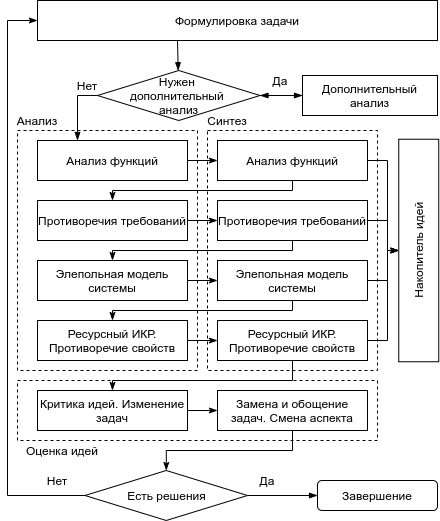
\includegraphics[scale=0.7]{DISSER-42.png}
    }
    \caption{АРИЗ Универсал 2010}\label{fig:ariz-1}
\end{figure}

Ключевые шаги АРИЗ Универсал 2010, состоят из следуюших этапов, указанных на Рисунке ~\cref{fig:ariz-2}:

\begin{enumerate}
	\item анализ задачи,
	\item синтез задачи,
	\item критическая оценка предлагаемого альтернативного решения.
\end{enumerate} 


\begin{figure}[ht]
    \centerfloat{
        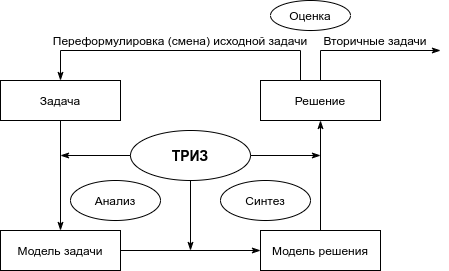
\includegraphics[scale=0.7]{DISSER-43.png}
    }
    \caption{АРИЗ Универсал 2010}\label{fig:ariz-2}
\end{figure}

Таким образом, таблица противоречий состоит из следующих каналов наблюдения и приложена к работе в Приложении ~\cref{app:B2}:

\begin{enumerate}
	\item вычислительные ресурсы (серверное оборудование, сеть, оборудование сопряженное, коммутация, техничесие средства ЭВМ, облачные ресурсы и т.д.),
	\item время обработки данных,
	\item скорость обработки данных,
	\item объем данных,
	\item количество запросов за единицу времени,
	\item количество пользователей/потребителей информации,
	\item нагрузка на систему,
	\item размер объектов, структурирующие данные,
	\item устойчивость элементов системы (пго конкретным элементам),
	\item устойчивость всей системы в целом,
	\item количество элеметнов, структурируюшие данные в системе,
	\item качество элементов системы,
	\item качество всей системы,
	\item надежность элементов системы,
	\item надежность всей системы в целом,
	\item информационная безопасность элементов системы,
	\item информационная безопасность всей системы,
	\item удобство экспуатации системы,
	\item удобство эксплуатации элементов системы,
	\item удобство изготовления элементов системы,
	\item удобство изготовления всей системы,
	\item удобство ремонта элементов системы,
	\item удобство ремонта всей системы в целом,
	\item удобство обновления элементов системы,
	\item удобство обновления всей системы в целом,
	\item удобство сопровождения элементов системы,
	\item удобство сопровождения всей системы,
	\item адаптация элементов системы,
	\item адаптация всей системы в целом,
	\item сложность разработки элементов системы,
	\item сложность разработки системы,
	\item сложность контроля и измерений состояний процессов,
	\item сложность вычислений,
	\item сложность использования ресурсов, 
	\item сложность использования объектов, структурирующих данные,
	\item степень автоматизации системы,
	\item производительность.
\end{enumerate}

Таким образом, перечисленные каналы наблюдения будут использоваться, как основные параметры для обучения алгоритма классификации и поиска максимального значения функионала производительности.


\subsection{Параметрический критерий нагрузки на автоматизированные системы}\label{sec:ch2/sec2/sub2}
Рассмотрим параметрический критерий нагрузки на системы, основанный на следующем свойстве экспоненциального распределения плотности 
\begin{equation}
    \label{eq:equation20}
    f(t) = \frac{1}{T}e^{(-1T)}, T = \sqrt{D}  
\end{equation}

где $T$ - математическое ожидание экспоненциального закона;

$D$ - дисперсия, определяемая по зависимости ~\cref{eq:equation21}
\begin{equation}
    \label{eq:equation21}
    D = \int_0^{\infty} \mathrm \{\frac{(1-T)^2}{T}e^{-\frac{1}{T}}\,\mathrm{d}t    
\end{equation}

Рассмотрим случай, когда на систему действует два источника нагрузки: пользовательская нагрузка, состоящая из поступающего на обслуживание через веб-сервер множество запросов и запросы командной нагрузки от сторонних платформ, поступающие через интеграционные шлюзы. Запросы проходят через доменные имена и распределяются в балансировщиках нагрузки, которые направляют входящие запросы на один из множества серверов приложения, которые обычно являются зеркальными копиями друг друга, и отправляют ответ обратно пользователю. Любой сервер обрабатывает запросы одинаково, так что балансировщик занимается распределением заданий, чтобы никакой из них не был перегружен.
Таким образом, в момент старта работы приложений запросы между пользователями могут соревноваться за ресурсы информационной системы. Для описания этого процесса воспользуемся двух-параллельным марковским процессом ~\cref{eq:equation22}
\begin{equation}
    \label{eq:equation22}
    M = [A, h(t)]  
\end{equation}
                       (3)
где $ A = \{a_{w1},a_{w2}, a_{g1},a_{g2} \}$ - множество состояний, 

$a_{w1}, a_{g1}$ - стартовые состояния, 

$a_{w2}, a_{g2}$ - поглощающие состояния, 

$h(t)$ - полумарковская матрица;

Для определения времени ожидания процесса воспользуемся описанием вида ~\cref{eq:equation23}


\begin{equation}
    \label{eq:equation23}
    M = [A', h'(t)]  
\end{equation}

где $A' = AB$ - множество состояний;

$A = \{\alpha_1, \alpha_2, \alpha_3\}$ - подмножество состояний, моделирующее начало и окончания блужданий по полумарковскому процессу; 

$\alpha_1$ - стартовое состояние;

$\alpha_2$ - поглощающее состояние, моделирующее выигрыш второго субъекта; 

$\alpha_3$ - поглощающее состояние, моделирующее окончание ожидания первым субъектом окончания второго;

$B = \{\beta_1,\beta_2, \beta_3 \}$ - бесконечное множество состояний, задающих временные интервалы ситуаций завершения обслуживания вторым
 $h'(t) = \{h'_{m,n}(t)\}$ - полумарковская матрица, задающая временные интервалы процесса.


Представим плотность распределения времени наблюдения за системой посредством закона вырожденного распределения с некоторым математическим ожиданием  $T$   и  $\omega(t) = \delta(t - T)$ , который соответствует некоторому детерминированному процессу. Таким образом, плотность распределения времени ожидания завершения события $g(t)$, определяется согласно зависимости ~\cref{eq:equation24}:


\begin{equation}
    \label{eq:equation24}
    f_{\delta \rightarrow g(t)} = \frac{\eta(t)g(t+T)}{\int_T^{\infty} \mathrm {g(t)}}\,\mathrm{d}t}
\end{equation}

Математическое ожидание имеет вид ~\cref{eq:equation25}:
\begin{equation}
    \label{eq:equation25}
    T_{\delta \rightarrow g(t)} = \int_0^{\infty} \mathrm {t\frac{g(t+T)}{\int_T^{\infth} \mathrm{g(t)\,\mathrm{d}t}}}\,\mathrm{d}t}
\end{equation}

Критерий, основанный на определении времени ожидания для строго детерминированной связи между событиями, выражаемой - функции Дирака $g(t) = \delta(t - T)$, имеет вид:
\begin{equation}
    \label{eq:equation26}
    \varepsilon_{\omega} = \frac{t-T_{\delta\rightarrow\g}}{T}^2 
\end{equation}

где $T$ - математическое ожидание анализируемой плотности распределения времени между соседними событиями; 

$T_{\delta\rightarrow g}$- математическое ожидание плотности распределения $f_{\delta\rightarrow g(t)}, рассчитываемое по зависимости ~\cref{eq:equation24}.

Математическое ожидание распределения сигнала определяется по следующей зависимости 
\begin{equation}
    \label{eq:equation27}
    T_k = \int_0^1 \mathrm{tK(1-t)^{K-1}}\,\mathrm{d}t = \frac{1}{K+1}[время]
\end{equation}

Экспоненциальный закон, определяющий Пуассоновский поток событий 
\begin{equation}
    \label{eq:equation28}
    f_K(t) = (K+1)e^{[-(K+1)t]} [probtime]
\end{equation}

\subsection{Групповой критерий надежности работы системы}\label{sec:ch2/sec2/sub3}

Рассмотрим задачу анализа надежности системы с точки зрения моделирования группового отказа в системе. Представим, что модель работы в какой-то момент времени начнет отказывать в обслуживании, т.е. модули системы или некоторый функционал начнет давать сбой. Назовем такое поведение, как вероятность наступления группового отказа в системе. Модулями в системе выступает допустимое множество решений модели поддержки принятия решений.
Пусть вероятность наступления события отказа представляется в виде $k$ вершин надежных решений, где связи между вершинами, а также сами вершины определяют вероятность выхода из строя. Количество вершин ограничено от двух до произвольного значения. Таким образом, модель примет вид графа с вершинами, где ребра и вершины отображают вероятность наступления отказа. Вероятность наступления отказа в модели, отображающей множество решений   
При проектировании автоматизированной системы управления задача определения надежности работы системы является одной из важнейших задач. В эту задачу входят такие важнейшие аспекты работы системы, как \cite{ACSSt}:
\begin{itemize}
	\item совместимость между частями,
	\item готовность к масштабированию,
	\item приспособленность к модернизации,
	\item надежность в установленных целях и в заданных условиях применения,
	\item адаптивность для лостижения поставленных целей работы системы,
	\item меры безопасности и обеспечение безопасности работы системы в целом.
\end{itemize}

Рассмотрим данную задачу с точки зрения неориентированного графа в аспекте абстрактной модели проектируемой автоматизированной системы, где в зависимости от конкретной цели и типа системы будет видоизменяться некоторый набор параметров в модели оценки надежности работы системы. В литературе известны примеры исследования таких задач с помощью методологий, основанных на так называемых $k$ - терминальных надежностей, где определяется вероятность выхода из строя вершин и узлов графа. Однако, согласно выводам из \cite{groupotkazy} такие модели зачастую упускают вероятностный выход из строя надежных вершин, а также слишком упрощают реальные условия выхода из строя системы, что приводит к их неадекватности отражения реальности. 
Наиболее реалистичными сценариями отказов, согласно наблюдениями из \cite{groupotkazy}, являются отказы, которые приводят к цепочке отказов, происходящих одновременно или со временем. В общем смысле, ошибка состоит в рассмотрении события отказа , как независимого события.

В данной работе предлагается рассмотреть модель случайного графа.  
Каждое ребро или вершина может выходить из строя. При выходе из строя граф или вершина не восстанавливаются, т.е. удаляются из графа: при отказе работы вершины - удаляется вершина со веми инцидентными ей ребрами, при отказе работы ребра - удаляется ребро из графа. Распространение отказа в графе происходит последовательно, кратно минимально возможному интервалу времени. Допускается наличие некоторого порогового уровня распространения отказа в системе, после которого распространение отказа блокируется автоматически, например, посредством некоторого механизма безопасности. 
Таким образом, модель представляется в следующем виде:
отказы происходят каскадно, т.е. вероятность отказа элемента на $i$ - ом шаге зависит от того, какой конкретно элемент вышел из строя на предыдущем $i - 1$ - ом шаге.
На первом шаге элементы отказывают независимо. 


\section{Математическая модель системы логического вывода}\label{sec:ch2/sec3}

Для построения экспертной системы используются следующие алгоритмы:
\begin{enumerate}
	\item алгоритм построения семантического графа объектов и признаков для обучения модели по прецендентам,
	\item алгоритм построения коллекции решающих деревьев на основе таблицы противоречий,
	\item алгоритм классификации на основе алгоритма случайного леса для нахождения конечного вектора ответов для функционала производительности по каналам наблюдения из таблицы противоречий,
	\item алгоритм подбора рекоммендаций методом максимального правдоподобия функционала производительности на основе матричный разложений и  ортогонолизации параметров из каналов наблюдения модели.
\end{enumerate}

Обучающая выборка представляется в виде семантического графа, вершины которого состоят из объектов, которыми являются каналы наблюдения, а ребра представляют связь между каналами. Каждому каналу наблюдения проставляется оценка значимости первоначально случайным образом. 

\subsection{Поиск информативных конъюнкций как задача отбора признаков}\label{sec:ch2/sec3/sub1}
Для поиска информативных конъюнкций требуется приспособить один из методов отбора признаков. Вместо минимазации ошибки воспользуемся критерием макисимума информативности. Воспользуемся логическим алгоритмом классификации и информативной конъюнкцией. Синтез параметров, как признаков из графа параметров и ТРИЗ таблицы противоречий будет производится посредством поиска закономерностей. Задача стоит отделить линейно независимые параметры от линейно зависимых. Для этого из параметров графа будет строится система непересекающих множеств на основе древовидных структур данных. Основным принципом и критерием классификации будет критерий максимума информативности.

Каналы наблюдения задаются в виде функционалов нечеткой логики Мамдани. Каждому параметру соответсвет значение нечеткого функционала.

Представим модель в виде некоторой нелинейной системы:
\begin{equation}
    \label{eq:equation36}
    \[ \varphi(y(x)) = \left\{\begin{array}{ll} x_i, i   = 0,1, ...,  n,\textrm{,}\\ y_k = f_y(x_1,x_2,...,x_n), k = 1,2,...,q & \end{array} \right. \]
\end{equation}

Представим множество возможных значений в следующем виде:
\begin{equation}
    \label{eq:equation37}
    U = \{u_j, u_{j+1},.., u_m\}
\end{equation}

где $u_j$ - оценка, которая проставляется в соответсвии с входной информацией в систему,

$m$ - мощность множества.

Решением задачи будет составление такого множества значений $Y*= \{y_1^*, y_2^*, ..., y_n^*\}$ на постившее множество $X* = \{x_1^*, x_2^*,...,x_n^*\}$. Таким образом, на множество, поступающих значений $X*$ формируется множство выходных значений $Y*$.
Для установления зависимости между объектами выразим эвристическую закономерность в виде обработки семантических лингвистических переменных. Для этого выразим объекты через некоторые терм множества:
\begin{equation}
    \label{eq:equation38}
    A = \{a_j, a_{j+1}, ..., a_m\}
\end{equation}
Данные семантические терм определяются на основе соотношения
\begin{equation}
    \label{eq:equation38}
    a_j = \sum_{p=1}^l\frac{\mu^{a_{j}(u^p_j)}}{u^p_j}
\end{equation}

$\mu^{a_{j}(u^p_j)}$ - степень принадлежности,

$u^p_j$ - объект принадлежности.

Степень принадлежности определяется на основе рангов принадлежности и определяется на основе соотношений следующей системы:
\begin{equation}
    \label{eq:equation40}
    \[ R(\mu) = \left\{\begin{array}{ll} \frac{\mu_1}{\r_1} = \frac{\mu_2}{\r_2} = ... = \frac{\mu_m}{\r_m}, i   = 0,1, ...,  m,\textrm{,}\\ \sum_{i=1}^m{\mu_i} = 1  & \end{array} \right. \]
\end{equation}
В соответствии с нормировкой находим:
\begin{equation}
    \label{eq:equation41}
    \[ R(\mu) = 
    \left\{\begin{array}{ll} 
    \mu_{n-1} = (1 + \frac{r_n}{r_{n-1}} + \frac{r_{n+1}}{r_{n-1}} + ... )^{-1} \textrm{,} 
    \\ \mu_{n+m} = (\frac{r_{n-1}}{r_n} + \frac{r_{n+1}}{r_n} + ... )^{-1}  & \end{array} \right. \]
\end{equation}

Получаемая матрица обладает следующими свойствами:
\begin{enumerate}
    \item транзитивность,
    \item симметричность,
    \item диагональность.
\end{enumerate}

На основании этих свойств выведем соотношение:
\begin{equation}
    \label{eq:equation42}
    s_{ij} = \frac{s_{kj}}{s_{ki}}
\end{equation}

На основе матрицы парных рангов составляется соотношение со значениями 9-ти бальной шкалы Саати 
На рисунке ~\cref{fig:ST} представлена 9-ти бальная шкала Саати.

\begin{figure}[ht]
    \centerfloat{
        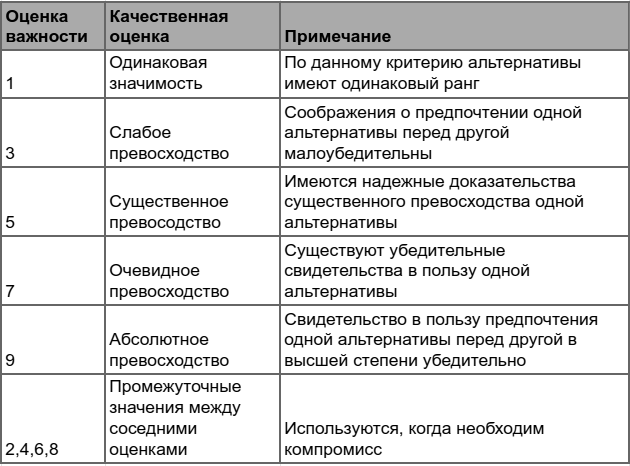
\includegraphics[scale=0.59]{Dissertation/images/APP-1.png}
    }
    \caption{9-ти бальная шкала Саати}\label{fig:ST}
\end{figure}

Приведем перечень функций принадлежности классов. Функция принадлежности к некоторому классу $s$ приведена в ~\cref{eq:equation43}.
\begin{equation}
    \label{eq:equation43}
    s(x,a,b,c) = \left\{\begin{array}{ll} 
    0, x\leq{a} \textrm{,} 
    \\ 2{\frac{x-a}{c-a}}^2, a\leq x\leq b    \\
    1 - 2{\frac{x-c}{c-a}}^2, b\leq x\leq c   \\ 
    1, x\geq c & \end{array} \right. \]
\end{equation}

где $b = \frac{a+c}{2}$.

Конъюнкционная закономерность интерпретируется на основе:
\begin{equation}
    \label{eq:equation44}
    (i): Q ; P; A \rightarrow B;S,F,N
\end{equation}

где $(i)$ - имя нечеткого  канала налюдения,

$Q$ - домен нечеткого канала налюдения,

$P$ - условия принятия, критерий принятия,

$A \rightarrow B$ - ядро конъюнкционой закономерности,

$B$ - результирующее заключение, следствие,

$\rightarrow$ - знак коньюнкционной секвенции,

$S$ - метод определения количественной истинности,

$F$ - коэффициент истины,

$N$ - ограничения конъюнкционного вывода.


База знаний в соответствии с представление в виде коньюнкционных правил образует совокупность множество, представимое в некоторой совокупности таблиц фактов.
Термы множества задаются с стандартной форме в виде логических отношений. База знаний задается в виде набора полей, объединенных некоторым логическим отношением, записанных в некоторой таблице совокупности фактов в виде графа, на основании которых выводится коньюнкционное правило.
Нечеткая база знаний может быть представлена в следующей виде в виде функции Мамдани:

\begin{equation}
    \label{eq:equation45}
    \bigcup_{p=1}^{t_k} [\bigcap_{i=1}^{n} \(x_i = a_j^{kp}\)]   \rightarrow  \bigcup_{p=1}^{t_k} [ \bigcap_{k=1}^{q} \(y_k = b_j^{kp}\)  ]
\end{equation}

где  $j = {1,2, ..., q}$, $k = {1,2, ..., q}$, $p = {1,2, ..., t_k}$

База знаний формируется в соответствии с Рисунком ~\cref{fig:KBase}. Структура матрицы знаний представлена с Рисунком ~\cref{fig:ST}.

\begin{figure}[ht]
    \centerfloat{
        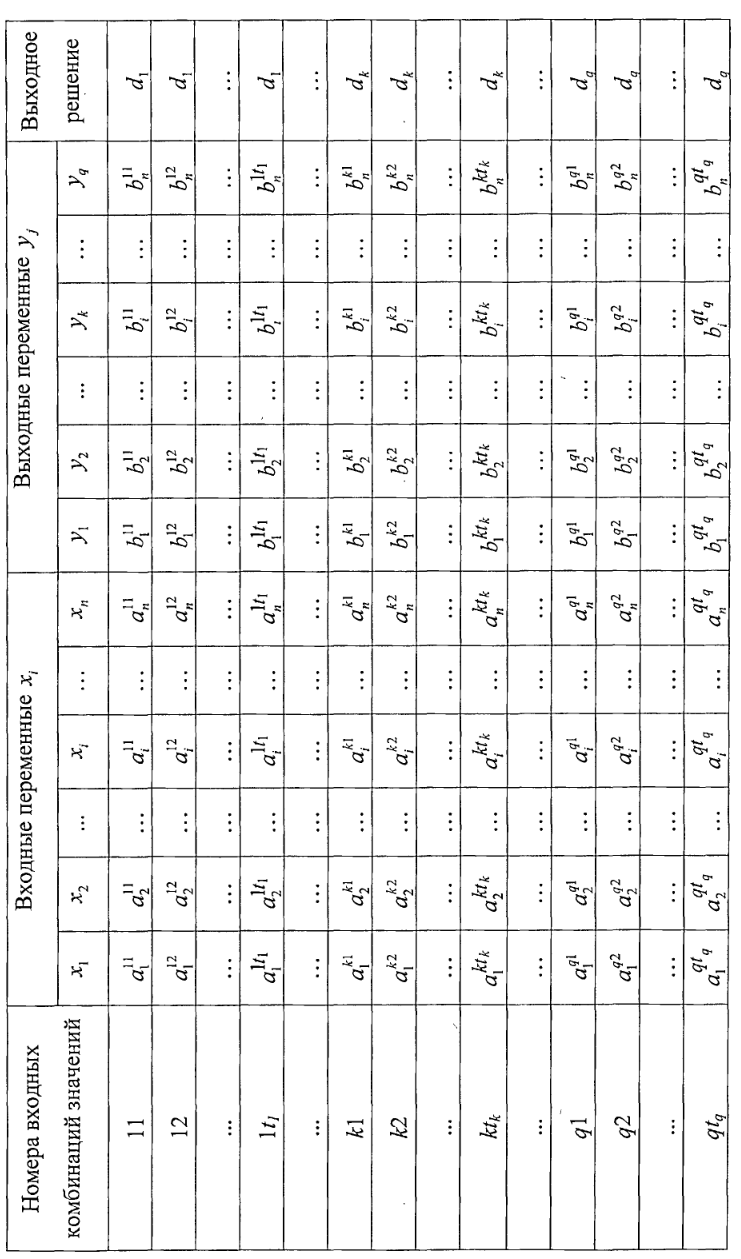
\includegraphics[scale=0.5]{Dissertation/images/DISSER-7.png}
    }
    \caption{Структура матрицы знаний}\label{fig:KBase}
\end{figure}

Система непересекающих множеств строится следующим образом:
\begin{enumerate}
	\item стоится дерево для множества, одно дерево соответсвует одному множеству,
	\item создается массив "родитель", на которого хранится ссылка, для корней дерева ссылка замыкается сама на себя,
	\item создается операция "$\rm make\_up$" добавляет новый элемент $ x $, помещая его в новое множество, состоящее из одного него,
	\item создается операция "$\rm union\_sets(x,y)$" объединяет два указанных множества (множество, в котором находится элемент $x$, и множество, в котором находится элемент $y$),
	\item создается операция "$\rm find\_set}(x)$" возвращает в каком множестве назодится объект - указанный элемент $x$.
\end{enumerate}

Если вызов $ {\rm find\_set}(x)$ для каких-то двух элементов вернул одно и то же значение, то это означает, что эти элементы находятся в одном и том же множестве, а в противном случае — в разных множествах.
Оценка асимптотики алгоритма будет логарифимческой на один запрос в среднем $ O (\log n)$ ~\cite{logn, tomaskormenm, kurtm, RobertEndreTarjan1, RobertEndreTarjan2}.

Алгоритм синтеза решающих деревьев правильно классифицирующих объекты по их признакам на классы является $NP$ - полной задачей.

В основе построения классификатора лежит прицнип индуктивного вывода логических закономерностей или индукции правил. 
Пусть $ \phi: X \rightarrow \{0,1\} $ некоторый предикат, который определяется на множестве объектов X. Предикат $ \phi $ является закономерностью и является неотемлимым атрибутом для построения закономерностей в процессе поиска правил по ваыборке и извлечения знаний из данных. К знаниям предъявляется особое требование -  интерпретируемость.

Всякая закономерность может классифицировать только некоторую часть объектов. Для того, чтобы классифицировать любые объекты требуется получить объединение закономерностей в некоторую композицию.  

Для поиска конъюктивных закономерностей в модели используется алгоритм построения логической классификации с помощью решающего дерева. Деревом называется конечный граф с множеством вершин $ V $, которые не содержат циклы и имеет вершину $ v_{0} \in V$, в которую ни одно ребро не входит. Такая вершина называется корнем дерева. Вершина, которая не имеет выходящих ребер, называется терминальной или листом. Остальные вершины называются внутренними.

Объект $x$ доходит до вершины $v$ при условии, что выполняется конъюнкция K_{v}(x) всех предикатов внутренних вершин дерева на пути от корня $v_{0}$ до вершины $v$. Пусть $T$ - множество всех терминальных вершин. Множества объектов $\Omega_{v} = {x \in X }$ выделяется терминальными конъюкциями $v \in T$. Объекты $x$ попарно не пересекаются, объединение объектов совпадает со всем пространством $X$.

Пусть $X $ - пространство объектов, $Y = \{1,2, ..., M\}$ - множество классов. Тогда, целевая зависимость $X $ от $Y$ задается в следующем виде: $X^{l} = (x_{i},y_{i})^l_{i=1}, y_{i} = y^*(x_{i})$. Алгоритм классификации $ a: X \rightarrow Y $ аппроксимирует $y^*$ на всем множестве $Y$.

В общем случае, ансамбль решающих деревьев строится на основе критерия
Введем значение количества объектов, как $N$, а количество признаков $ D $. Пусть $L$ - число отдельных моделей в ансамбле. Для каждой отдельной модели $l$ выбирается $dl (dl < D)$, такой дифференциал представляет собой число признаков для $l$. Для всех моделей, по умолчанию, выбирается одно значение $dl$. Для каждой отдельной модели $l$ создается обучающая выборка посредством выбора $dl$ признаков из $D$ для обученяи модели. Далее, для применения модели к новому объекту следует объединить результаты отдельных $L$ моделей путем мажоритарного голосования:

\begin{equation}
    \label{eq:equation29}
    a(x) = argmax_{\substack{ y \in Y
  }} \sum_{\substack{
   v \in V \\
   Cv = y
  }} 
 K_{v}(x)
\end{equation}

\subsection{Критерий максимума информативности}\label{sec:ch2/sec3/sub3}

Предикат $\phi$ называется информативным, если он отбирает наибольшее количество объектов одного классов $c \in Y$, к которому принадлежит, по сравнению с объектами другого класса. Объекты одного класса, которому называются позитивными, а чужие негативными. Введем обозначения следующего вида, согласно Рисунку ~\cref{fig:inform}.

Пусть $P_c$ - число объектов класса $c$ в выборке $X^{l}$; $p_c(\phi)$ из них число объектов, для которых выполняется условие $\phi(x) = 1 $; $N_c$ число объектов всех остальных классов $Y \ \{c\}$ в выборке $X^{l}$; $n_c(\phi)$ из них число объектов, для которых выполняется условие $\phi(x) = 1 $.

Предполагается, что $P \geq 1$, $N \leq 1$, $P + N = l$.

\begin{figure}[ht]
    \centerfloat{
        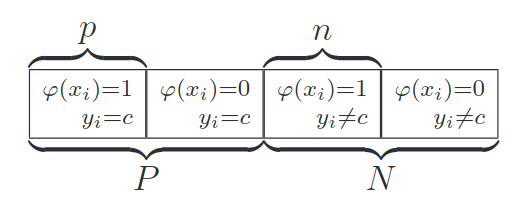
\includegraphics[scale=0.6]{Dissertation/images/DISSER-44.png}
    }
    \caption{О понятии информативности}\label{fig:inform}
\end{figure}

Мера информативности определяется какое количество позитивных объектов он выделяет. Задача построения информативного предиката $\phi$ формулируется посредством следующих задач оптимизации:

\begin{equation}
    \label{eq:equation30}
   p_{c}(\phi) \rightarrow max 
\end{equation}

\begin{equation}
    \label{eq:equation31}
    n_{c}(\phi) \rightarrow min
\end{equation}

Позитивные объекты, выделенные предикатом задаются в виде:

\begin{equation}
    \label{eq:equation32}
    D_{c}(\phi, X^{l}) = \frac{p_{c}(\phi)}{l}
\end{equation}

Негативные объекты, выделенные предикатом задаются в виде:

\begin{equation}
    \label{eq:equation33}
    E_{c}(\phi, X^{l}) = \frac{n_{c}(\phi)}{p_{c}(\phi) + n_{c}(\phi)}
\end{equation}

Предикат \phi(x) называется логической $\epsilon, \delta$ - закономерностью для класса $c \in Y $, если $E_{c}(\phi, X^{l}) \leq \epsilon $ и 
$D_{c}(\phi, X^{l}) \geq \delta $ при заданном достаточно малом \epsilon и достаточно большом \delta из отрезка $[0,1]$.

Если $n_{c}(\phi) = 0$, то закономерность \phi называется чистой или непротиворечивой. Если $n_{c}(\phi) > 0$, то закономерность \phi называется частичной.

Информативность предиката \phi(x) относительно класса $c \in Y$ по выборке $ X^{l}$:

\begin{equation}
    \label{eq:equation34}
    I_{c}(\phi, X^{l}) = -ln h \Bigg(
    \begin{matrix}
    p_{c}(\phi) & n_{c}(\phi) \\
    P_{c} & N_{c}
    \end{matrix}
    \Bigg)
\end{equation}

При этом следует учесть, что $ I_{c} \equiv I_{c}(\phi) \equiv I_{c}(\phi, X^{l}) $.

Сформулируем статистическое определение информативности посредством техники проверки статистических гипотез. Пусть $X$ - вероятностное пространство , выборка $X^{l}$ - простая, то есть случайная, независимая, одинаково распределенная, $y^{*}(x), \phi(x)$ - случайные величины.
 Допустим, что гипотеза о независимости событий справедлива:

\begin{equation}
    \label{eq:equation35}
    \{x: y^*(x) = c\} , \{x: \phi(x) = 1\}
\end{equation}

Тогда вероятность реализации пары $(p, n)$ возможно выразить через следующее гиперпараметрическое распределение:

\begin{equation}
    \label{eq:equation36}
    \left h\Bigg( 
    \begin{matrix}
    p & n \\
    P & N
    \end{matrix}
     \Bigg)
    =
    \frac{C_P^p C_N^n}{C^{p+n}_{P+N}}, 0 \leq p \leq P, 0 \leq n \leq N \right
\end{equation}

где

\begin{equation}
    \label{eq:equation37}
    C^{k}_m = \frac{m!}{k!(m-k)!}, 0 \leq k \leq m.
\end{equation}

Таким образом, если событие с малой вероятностью реализовалось, то, скорее всего, оно не случайно. Неслучайное событие это и есть закономерность.

Определим информативность предиката \phi(x) относительно класса $c \in Y $ по выборке $X^{l}$:

\begin{equation}
    \label{eq:equation38}
    I_c(\phi, X^{l}) = - ln h \Bigg(
    \begin{matrix}
    p_c(\phi) & n_c(\phi) \\
    P_c & N_c
    \end{matrix}
    \Bigg)
\end{equation}

Предикат \phi(x) будем называть статистической закономерностью для класса $c$ в случае, если при заданном достаточно большом $I_0$ справедливо следующее неравенство:

\begin{equation}
    \label{eq:equation39}
    I_c(\phi, X^{l}) \geq I_0
\end{equation}


Уровень значимости для порога информативности $I_0$ выбирается достаточно малым для проверки статистических гипотез о независимости событий.

Для вычисления информативности воспользуемся приближенным методом расчета Стирлинга:
\begin{equation}
    \label{eq:equation40}
    ln k! \approx \Bigg( k + \frac{1}{2} \Bigg) ln k - k + \frac{1}{2}ln2\pi + \frac{1}{12k} - \frac{1}{360k^2}
\end{equation}

Существует два исхода $\omega_{0}, \omega_{1}$ с вероятностями $q_{0}$ и $q_{1} = 1 - q_{0}$. Количество информации, связанное с исходом $\omega_{i}$ равно $-log_{2}(q_{i})$.

Энтропия определяется, как математическое ожидание от количества информации:

\begin{equation}
    \label{eq:equation41}
    H(q_0, q_1) = - q_{0}log_{2}q_{0} - q_{1}log_{2}q_{1}
\end{equation}

Появление объекта класса $c$ с исходом $\omega_0$, а появление любого другого класса $\omega_1$. Энтропия выборки X^{l} вычисляется на основе оценки вероятности исходов, как частоты:

\begin{equation}
    \label{eq:equation42}
    \widehat{H}(P,N) = H \Bigg(\frac{P}{P+N}, \frac{N}{P+N} \Bigg)
\end{equation}

Таким образом, после получения информации $\phi$ энтропия всей выборки становится равной:

\begin{equation}
    \label{eq:equation43}
    \left \widehat{H}(P,N,p,n) = \frac{p+n}{P+N}\widehat{H}(p,n) + \frac{P+N-p-n}{P+N}\widehat{H}(P-p, N-n)\right
\end{equation}

Уменьшение энтропии принимет вид и называется информационным выигрышем:

\begin{equation}
    \label{eq:equation44}
    IGain_{c}(\phi, X^{l}) = \widehat{H}(P,N) - \widehat{H}_{\phi}(P,N,p,n)
\end{equation}

Предикат \phi является закономерностью по энтропийному критерию информативности, если $IGain_{c}(\phi, X^{l}) > G_{0}$ при некотором достаточно большом $G_{0}$. Энтропийный критерий асимптотически эквивалентен статистическому:

\begin{equation}
    \label{eq:equation45}
    IGain_{c}(\phi, X^{l}) \rightarrow \frac{1}{l ln 2}I_{c}(\phi, X^{l}), при l \rightarrow \infty
\end{equation}

Статистический критерий информативности на случай произвольного числа классов $Y = {1,...,M}$:

\begin{equation}
    \label{eq:equation46}
    \left I(\phi, X^{l}) = -ln\frac{C^{p_{1}}_{P_{1}} ... C^{p_{M}}_{P_{M}}}{C^{p}_{l}}\right
\end{equation}

где $P_{c}$ - число объектов класса $c$ в выборке $X^{l}$, из них $p_{c}$ объектов выделяются предикатом $\phi, p = p_1 + p_2 + p_3 + ... + p_M$.

Энтропийный критерий для произвольного числа классов принимает вид и имеет асимптотическое приближение к статистическому:

\begin{equation}
    \label{eq:equation47}
    \left I(\phi, X^{l}) = \sum_{c \in Y} h \Bigg(\frac{P_c}{l} - \frac{p}{l}\sum_{c \in Y}h \Bigg( \frac{p_{c}}{p} \Bigg) - 
    \frac{l-p}{l}\sum_{c \in Y} h \Bigg(\frac{P_c - p_c}{l - p}\Bigg)\Bigg)  \right
\end{equation}

где $h(z) \equiv - z log_{2} z$.

Для выявления закономерностей используется алгоритм бустинга адаптированный для взвешенного голосования. В бустинге строятся последовательные закономерности, после построения очередного вектора весов закономерностей вектор пересчитывается. Веса выделенных для закономерностей объектов изменяются: у позитивных уменьшаются, у негативных увеличиваются. Обновленный вектор  весов $\omega$ используется при поиске следующей закономерности $\phi$ по критерию максимума взвешенной информативности.
Веса объектов и веса закономерностей на каждом шаге алгоритма изменяеются согласно критерию взвешенной информативности~\cref{eq:subeq_1, eq:subeq_2}.

\begin{subequations}
    \label{eq:subeq_1}
    \begin{gather}
        P_{c}^{\omega} = \sum_{i=1}^{l}\omega_{i}[y_{i} = c]; \label{eq:subeq_1-1} \\
        p_{c}^{\omega}(\phi) = \sum_{i=1}^{l}\omega_{i}[y_{i} = c][\phi(x_{i}) = 1]
    \end{gather}
\end{subequations}

\begin{subequations}
    \label{eq:subeq_2}
    \begin{gather}
       N_{c}^{\omega} = \sum_{i=1}^{l}\omega_{i}[y_{i} = c]; \label{eq:subeq_2-1} \\
       n_{c}^{\omega}(\phi) \neq \sum_{i=1}^{l}\omega_{i}[y_{i} = c][\phi(x_{i}) = 1]
    \end{gather}
\end{subequations}


где $\omega$ веса объектов $\omega = (\omega_i)^{l}_{i=1}$,

условие нормировки имеет вид $\sum^{l}_{i=1}\omega_{i} = l$ ,

$P^{\omega}_c$ - число объектов класса $c$ в выборке $X^{l}$,

$p^{\omega}_c$ - из них число объектов, для которых выполняется условие $\phi(x) = 1$,

$N_{c}^{\omega}$ - число объектов всех остальных классов $Y  {c}$ в выборке $X^{l}$,

$n_c^{\omega}(\phi)$ - из них число объектов, для которых выполняется условие $\phi(x) = 1$.

Гипергеометрическое распределение будет вычисляться по следующей формуле:

\begin{equation}
    \label{eq:equation48}
    ln \(z\)! \approx ([z+1] - z)ln[z]! + (z - [z])ln[z+1]!, z \in \mathbb{R}
\end{equation}

\subsection{Модель Библиотекаря для классификации}\label{sec:ch2/sec4/sub4}


Цель - разработать модель в соответствии с вышеописанными принципами:
для этого необходимо входным переменным $X = {x_1, x_2, ..., x_n}$ поставить в соответствие выходные $Y = {y_1, y_2, ..., y_n}$. Первым необходимоым принципом является преобразование базы знаний. Данная операция изображена на Рисунке ~\cref{fig:NNprin}.
\begin{figure}[ht]
    \centerfloat{
        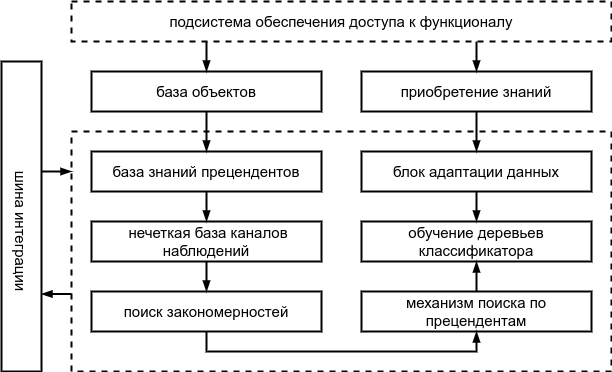
\includegraphics[scale=0.8]{Dissertation/images/DISSER-56.png}
    }
    \caption{Структура принципа преобразования}\label{fig:NNprin}
\end{figure}

Модель классификатора состоит из следующих алгоритмических блоков и называется "моделью Библиотекаря" так как основным ядром классификации является критерий максимума информативности:

\begin{enumerate}
	\item генерация обучающих выборок из каналов наблюдения таблицы ТРИЗ с помощью алгоритма бутстрепа, изображенного на Рисунке ~\cref{fig:bootstrap},
	\item вычисление списков закономерностей с выявлением значения весовых функций для каждого класса из обучающей выборки с помощью алгоритма бустинга,
	\item синтез решающего дерева на основе списков закономерностей для каждого класса,
	\item классификация параметров или каналов наблюдения по критерию максимума информативности,
	\item составление ансамбля деревьев для голосования согласно принципу максимума взвешенной информативности.
\end{enumerate}


\begin{figure}[ht]
    \centerfloat{
        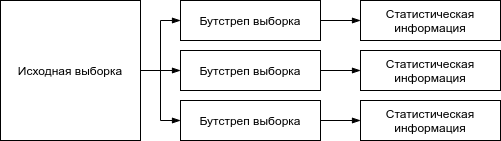
\includegraphics[scale=1.0]{Dissertation/images/DISSER-46.png}
    }
    \caption{генерация обучающих выборок с помощью алгоритма бутстрепа}\label{fig:bootstrap}
\end{figure}

Алгоритм бутстрепа позволяет выявить списки закономерностей на основе построения выпуклой комбинации закономерностей. Этот алгоритм последовательно строит закономерности, при этом на каждом этапе построения весовые коэффициенты закономерностей обновляются согласно критерию максимума взвешенной информативности. 

Для проведения обучения на обучающей выборке в модели используется алгоритм бустинга. Для определения закономерности, которая совершает минимальное количество ошибок на обучающей выборке $X^{l}$  распишем функционал числа ошибок алгоритма $a_{T+1}(x)$, с помощью тождества 
$e^{A\phi} = (1-\phi)+\phi e^{A}, A \in \textbb{R}, \phi \in {0,1} $:

\begin{equation}
    \label{eq:equation51}
     \begin{multlined}
    \tilda{Q}_{T+1} = \sum_{i=1}^{l}\omega_{i}e^{-\alpha\phi_c(x_i)}[y_{i} = c] + \sum_{i=1}^{l}\omega_{i}e^{\alpha\phi_c(x_i)[y_i \neq c]} = \\
    = \sum_{i=1}^{l}\omega_{i}(1-\phi_c(x_i)) + e^{-\alpha}\sum_{i=1}^{l} \omega_{i} \phi_c(x_i) [y_{i} = c] +
    \\
    + e^{\alpha}\sum_{i=1}^{l}\omega_{i}\phi_{c}(x_i)[y_i \neq c]
     \end{multlined}
\end{equation}

Выразим минимум этого функционала , который достигается при $e^{-\alpha}p = e^{\alpha}n$, $\alpha^* = \frac{1}{2}ln\frac{p}{n}$:
\begin{equation}
    \label{eq:equation52}
    \begin{multlined}
    \tilda{Q}_{T+1} = \frac{\tilda{Q}_{T}}{l} \Bigg( \sum_{i=1}^{l}\tilda{\omega}_{i} - \sum_{i=1}^{l}\tilda{\omega}_{i}\phi_{c}(x_{i}) +
    \\
    +
    e^{-\alpha}\sum_{i:y_{i}=c}\tilda{\omega}_{i}\phi_{c}(x_{i}) + e^{\alpha}\sum_{i:y_{i} \neq c}\sum_{i:y_{i} \neq c}\tilda{\omega}_{i}\phi_{c}(x_i)  \Bigg) = \\
    = \frac{\tilda{Q}_{T}}{l} (l - p^{w}_{c}(\phi_c) - n^{\omega}_c(\phi_c) + e^{-\alpha}p^{w}_{c}(\phi_c) +e^{\alpha}n^{\omega}_c(\phi_c))
    \end{multlined}
\end{equation}

Минимум достигается при $e^{-\alpha}p^{w}_{c}(\phi_c) = e^{\alpha}n^{\omega}_c(\phi_c)$, где $\alpha^* = \frac{1}{2}ln{\frac{p}{n}}, n \neq 0$:
\begin{equation}
    \label{eq:equation53}
    \begin{multlined}
    \tilda{Q}_{T+1} = \frac{\tilda{Q}_T}{l} \Bigg( l - p^{w}_{c}(\phi_c) - n^{\omega}_c(\phi_c) + 
    \\
    + p^{w}_{c}(\phi_c)\sqrt{\frac{ n^{\omega}_c(\phi_c)}{p^{w}_{c}(\phi_c)}} + n^{\omega}_c(\phi_c) \sqrt{\frac{p^{w}_{c}(\phi_c)}{ n^{\omega}_c(\phi_c)}}\Bigg) =
    \\
    = \tilda{Q}_{T}\Bigg( 1 - \frac{1}{l} (\sqrt{p^{w}_{c}(\phi_c)} - \sqrt{n^{\omega}_c(\phi_c)})^{2} \Bigg)
    \end{multlined}
\end{equation}

Для того, чтобы избежать неограниченного убывания функционала $\tilda{Q}_{T+1}$ при $n = 0$, введем дополнительный параметр $\lambda \in {0,1}$ для расчета формулы весов:
\begin{equation}
    \label{eq:equation54}
    \alpha^* = \frac{1}{2}ln\frac{{p^{w}_{c}(\phi^{*}_{c})}}{max \{n^{\omega}_c(\phi^*_c), \lambda\}}
\end{equation}

Таким образом, закономерность \phi определяется как:
\begin{equation}
    \label{eq:equation55}
    J^{\omega_c}_c(\phi_c) = \sqrt{p^{w}_{c}(\phi_c)} - \sqrt{n^{\omega}_c(\phi_c)}
\end{equation}

Веса закономерностей пересчитываются следующим образом:
\begin{equation}
    \label{eq:equation56}
    {\omega'}_{i} = \omega_i\Bigg( [y_i = c] e^{−\alpha\phi_c(x_i)} 
    + [y_i \neq c] e^{\alpha\phi_c(x_i)}] \Bigg) 
\end{equation}


\begin{equation}
    \label{eq:equation57}
\[ {\omega'}_{i} = \begin{cases}
    \omega_{i},       & \phi_c(x_i) = 0; \\
    \omega_{i}e^{-\alpha},       & \phi_c(x_i) = 1, y_i = c; \\
    \omega_{i}e^{\alpha},       & \phi_c(x_i) = 1, y_i \neq c; 
  \end{cases}
\]
\end{equation}


Принцип голосования основывается на подсчете голосов следующим образом, указанным на Рисунке ~\cref{fig:voting}. Пусть множество правил $ R_{c}$ или логических закономерностей для каждого класса $c \in Y$ будет описано в соответствии со следующей формулой:

\begin{equation}
    \label{eq:equation49}
    R_{c} = {\phi_{c}^{t}: X \rightarrow {0,1} | t = 1, ..., T_{c}}
\end{equation}

\begin{figure}[ht]
    \centerfloat{
        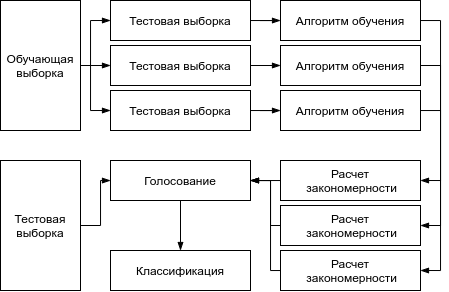
\includegraphics[scale=1.0]{Dissertation/images/DISSER-47.png}
    }
    \caption{Принцип голосования }\label{fig:voting}
\end{figure}

Тогда, если $\phi^{t}_{c} = 1 $, то это значит, что правило $\phi^{t}_{c}$ относит объект $x \in X$ к классу $c$. Если $\phi^{t}_{c} = 1 $, то классификации не происходит.

Голосование присходит следующим образом: каждому правилу $\phi^{t}_{c}$ приписывается вес $\alpha_{c}^{t} \geq 0$ и расчитывается взвешенная сумма голосов:

\begin{equation}
    \label{eq:equation50}
    \Gamma_c(x) = \displaystyle\sum_{t=1}^{T_c} \alpha_c^t\phi_c^t(x), \alpha_c^t \geq 0
\end{equation}

Веса нормируются до единицы $\displaystyle\sum_{t=1}^{T_c}\alpha_c^t = 1$ для всех $c \in Y$. Таким образом фнукция подсчета взвешенного голосования образует выпуклую комбинацию правил  $\phi_c^1 ,  ... , \phi_c^t$.

\subsection{Требования к модели}\label{sec:ch2/sec3/sub5}
Проектирование архитектуры автоматизированной системы является наиболее абстрактным и наиболее идеализированным представлением системы, которое должно обеспечивать выполнение следующих свойств:
\begin{enumerate}
\item элементы архитектуры должны быть слабо связаны таким образом, чтобы разложив на декомпозицию элементов, поток информации, проходящий по контурам был минимальным и не замыкался;
\item должно соблюдаться свойство тестируемости, т.е. при проверки работы функций системы должен быть установлен факт правильной работы;
\item должна соблюдаться возможность идентификации неисправных частей системы путем диагностики;
\item должно соблюдаться свойства восстановления системы в кратчайшие сроки с экономически обоснованной стоимостью ремонта;
\item должно соблюдаться свойство надежности;
\item система должна быть проста в обслуживании и проста в эксплуатации, не требовать высокой квалификации и повышения квалификации обслуживающего персонала;
\item система и ее составляющие элементы должны быть безопасны в эксплуатации, должны соблюдать требования охраны труда и техники безопасности;
\item система должны быть обеспечена защитой от вандализма и неавторизованных пользователей;
\item система должна проектироваться с учетом эффективности в отношении затрачиваемых ресурсов в  операционном процессе;
\item система должна уметь выстаиваивать новые конфигурации, создавать новые настройки для работы с другими технологическими процессами;
\item система должна уметь функционально расширяться, т.е. в логика работы должна уметь дополняться дополнительными функциональными возможностями системы;
\item система должны быть готова к устойчивому масштабированию системы, таким образом, чтобы увеличение размера объекта автоматизации не требовало высоких затрат и не сводила к неустойчивому состоянию базовую модель системы;
\item система должна быть открытой, таким образом, чтобы можно было заменить один модуль системы на аналогичный модуль другого производителя, а интеграция модулей происходила без чрезмерных конфликтов и проблем;
\item система должна стремиться к максимально продолжительному жизненному циклу без значительного устаревания, который должен обновлять аппаратные и программные компоненты;
\item система должна устанавливаться и вводиться в эксплуатацию за минимальное время.
\end{enumerate}

Таким образом, модель должна соблюдать перечисленные выше технические требования.

Принцип реализации сводится к адаптации информации, сформированной на базе фактов с пользовательским запросом на обработку и выдачу рекомендаций по проектированию. Общая схема движения информационного потока представлена на Рисунке~\cref{fig:Dataflow} 

\begin{figure}[ht]
    \centerfloat{
        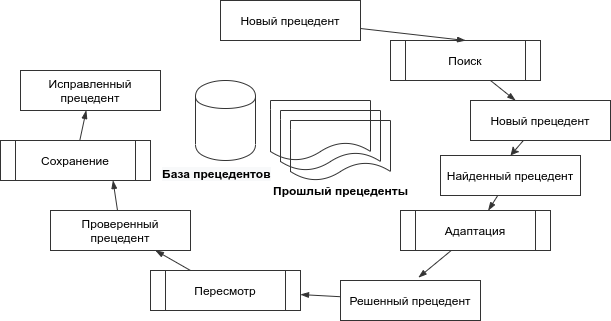
\includegraphics[scale=0.8]{Dissertation/images/DISSER-16.png}
    }
    \caption{Структура принципа преобразования}\label{fig:Dataflow}
\end{figure}
Для построения модели накладываются следующие ограничения:
\begin{enumerate}
	\item критерий максимума взвешенной информативности, позволяющий определить предикаты, как закономерности~\cref{eq:subeq_1, eq:subeq_2},
	\item критерий поиска конъюктивных закономерностей для отбора признаков ~\cref{eq:equation55, eq:equation56},
	\item мера информативной энтропии ~\cref{eq:equation47},
	\item экспоненциальная аппроксимация пороговой функции потерь ~\cref{eq:equation54}.
\end{enumerate}

Требования для разработки системы поддержки принятия решений вырабатываются на основе анализа проблем в области задачи принятия решений. Например, для поддержки принятия решений в области проектирования программного обеспечения крайне сложно анализировать организацию шаблонов проектрования кода на уровне отношений между сущности, также довольно сложнореализуемой задачей является анализ индексации таблиц и определения внешний и составных ключей, отношений между таблицами в БД.

Таким образом, основными требованиями при разработке модели поддержки принятия решений выступили требования по формированию вектора рекомендаций для проектирования того или иного набора инструментов для реализации задач проектирования. Для решения такой задач, после проведения анализа проблематики и выявления альтернатив, была разработана модель классификации на основетаблицы ТРИЗ, где каналы наблюдения выражены посредством инструмента нечеткой логики. Требования к модели принятия решений блоком классификатора, главным образом, определялся возможностью реализации конъюнкционного вывода на основе поиска закономерностей, но с возможностью обновления и адаптации под пользовательские запросы. Система должна уметь адаптироваться под запросы пользователей, а также адаптировать свою семантическую структуру закономерностей дополняя базу новыми наблюдениями, новыми прецендентами.

Основные требования при проектирования модели поддержки принятия решений перечислены здесь:

\begin{enumerate}
	\item система должна уметь интерпретировать слабоструктурированный текст в семантически верную закономерность,
	\item система должна уметь выявлять эвристические закономерности и аппроксимировать функционал оптимизации подбора рекомендаций,
	\item система должна уметь выявлять закономерности,
	\item система должна уметь обрабатывать отношения между объектами,
	\item система должна уметь формировать рекомендацию.
\end{enumerate}


\subsection{Алгоритмическое описание модели}\label{sec:ch2/sec4/sub2}

Цель - разработать алгоритм в соответствии с вышеописанными принципами:
для этого необходимо входным переменным $X = {x_1, x_2, ..., x_n}$ поставить в соответствие выходные $Y = {y_1, y_2, ..., y_n}$. Первым необходимоым принципом является преобразование базы знаний. Данная операция изображена на Рисунке ~\cref{fig:NNprin}.
\begin{figure}[ht]
    \centerfloat{
        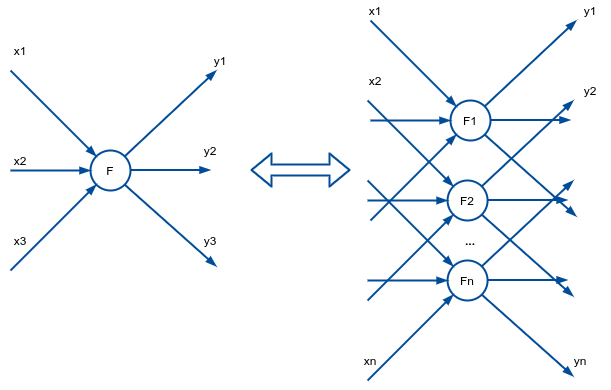
\includegraphics[scale=0.5]{Dissertation/images/DISSER-18.png}
    }
    \caption{Структура принципа преобразования}\label{fig:NNprin}
\end{figure}

Обобщенный алгоритм классификатора приведен на Рисунке~\cref{fig:commonclassificator}

\begin{figure}[ht]
    \centerfloat{
        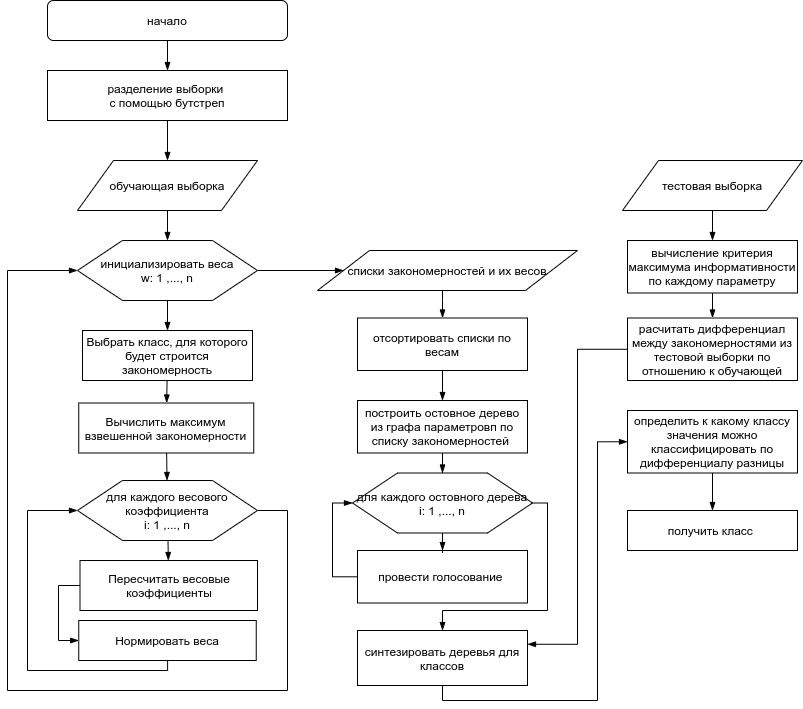
\includegraphics[scale=0.6]{Dissertation/images/DISSER-49.png}
    }
    \caption{Обобщенный алгоритм классификатора }\label{fig:commonclassificator}
\end{figure}


\begingroup
\centering
\small
\captionsetup[table]{skip=7pt} % смещение положения подписи
\begin{longtable}[c]{|l|c|l|l|}
    \caption{Алгоритмическое описание модели}\label{tab:test5}% label всегда желательно идти после caption
    \\[-0.45\onelineskip]
    \hline
    Шаг & Знач. по ум.& Тип & Описание                                          \\ \hline
    \endfirsthead%
    \caption*{Продолжение таблицы~\thetable}                                    \\[-0.45\onelineskip]
    \hline
    Шаг & Знач. по ум. & Тип & Описание                                          \\ \hline
    \endhead
    \hline
    \endfoot
    \hline
    \endlastfoot
    \multicolumn{4}{|l|}{\&INP}                                                 \\ \hline
    Входные     &       & double & 0: инициализация без шума (\(p_s = const\))\\
    данные         &        &     & 1: генерация и случайный отбор данных \\
             &        &     & из общих наблюдений \\
             &        &     & 2: применение операции случайного выбора \\
             &        &     & выборки из совокупности \\
             &        &     & 3: процедура перевыбора выборкив в цикле         \\
             &        &     & 4: вычисление среднего в цикле       \\
             &        &     & по каждой выборке                         \\
             &        &     & 2: генерация белого шума симметрично относительно \\
             &        &     & экватора                                          \\
    Поиск    & rand   & double & 0: инициализация весов случайными значениями   \\
    законо-  &        &     & или по оценкам       \\
    мернос-  &        &     & 1: выбор класса для построения закономерности    \\
    тей      &        &     & в цикле \\
    в обу-   &        &     & 2: внутри каждого выбранного класса рассчитать \\
    чающей   &        &     & $\phi^t_c = argmax_{\phi \in \Phi}\sqrt{\phi^w_c(\phi) - \sqrt{n^w_c(\phi)}}$\\
    выборке  &        &     & 4: внутри каждого выбранного класса рассчитать \\
             &        &     & $\alpha^t_c = \frac{1}{2}ln\frac{{p^{w}_{c}(\phi^{*}_{c})}}{max \{n^{\omega}_c(\phi^*_c), \lambda\}}$\\
             &        &     & 5: для всех $i = 1,...,l $  пересчитать вес \omega_i$ \\
             &        &     & 6: для всех $i = 1,...,l $  нормировать вес \omega_i$ \\
    Голо-    &        &double& 1: для всех $i = 1,...,l $  деревьев   \\
    вание    &        &     & 2: для каждой закономерности $\phi^{t}_{c}$ \\
             &        &     & приписывается вес $\alpha_{c}^{t} \geq 0$  \\
             &        &     & 3: расчитывается взвешенная сумма голосов         \\
             &        &     & $ \Gamma_c(x) = \displaystyle\sum_{t=1}^{T_c} \alpha_c^t\phi_c^t(x), \alpha_c^t \geq 0$\\
\end{longtable}
\normalsize% возвращаем шрифт к нормальному
\endgroup

Алгоритм бутстрепа состоит из следующих шагов и изображен на Рисунке ~\cref{fig:bootstrap}:
\begin{enumerate}
	\item формируется случайная выборка на основе генеральной совокупности из общего числа наблюдений,
	\item к каждой отобранной выборке применяется случайная операция выбора с возвратом того же размера,
	\item процедура перевыбора применяется многократное количество раз и выбирается среднее,
	\item из вычисленных средних по всем наборам вычислить среднее и рассматривать как среднее из генеральной совокупности.
\end{enumerate}

Алгоритм построения бустинга состоит из следующих шагов, изображенных на Рисунке  ~\cref{fig:busting}:
\begin{enumerate}
	\item на вход подается $X^l$ обучающая выборка, $\Phi$ семейство базовых предикатов, $T$ семейство базовых предикатов, $\lambda$ - коэффициеннт поощрения непротиворечивых закономерностей,
	\item на втором шаге инициализируются веса $\omega_i : = 1 $  для всех $i = 1, 2, ... , l$,
	\item далее для всех $t = 1, ... , T$ выбрать класс, для которого строится закономерность $c: c_t$:
	\begin{enumerate}
		\item внутри каждого выбранного класса рассчитать $\phi^t_c = argmax_{\phi \in \Phi}\sqrt{\phi^w_c(\phi) - \sqrt{n^w_c(\phi)}}$,
		\item внутри каждого выбранного класса рассчитать $\alpha^t_c = \frac{1}{2}ln\frac{{p^{w}_{c}(\phi^{*}_{c})}}{max \{n^{\omega}_c(\phi^*_c), \lambda\}}$,
		\begin{itemize}
			\item для всех $i = 1,...,l $  пересчитать вес \omega_i$,
			\item нормировать веса.
		\end{itemize}
	\end{enumerate}
\end{enumerate}

\begin{figure}[ht]
    \centerfloat{
        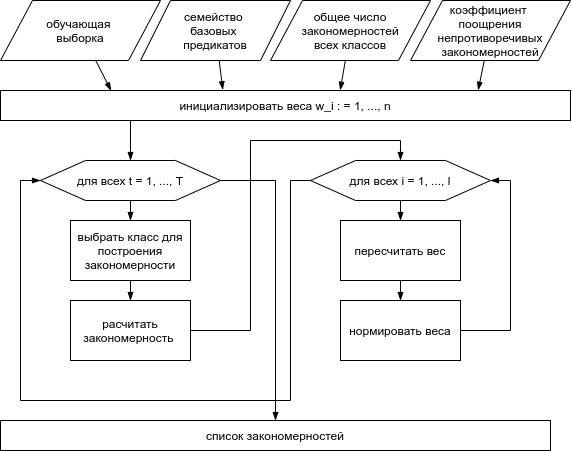
\includegraphics[scale=0.7]{Dissertation/images/DISSER-50.png}
    }
    \caption{Алгоритм построения бустинга }\label{fig:busting}
\end{figure}

Алгоритм голосования состоит из следующих шагов:
\begin{enumerate}
	\item для каждого дерева $i = 1, ..., n$:
	\begin{enumerate}
		\item для каждой закономерности $\phi^{t}_{c}$ приписывается вес $\alpha_{c}^{t} \geq 0$,
		\item расчитывается взвешенная сумма голосов $ \Gamma_c(x) = \displaystyle\sum_{t=1}^{T_c} \alpha_c^t\phi_c^t(x), \alpha_c^t \geq 0$.
	\end{enumerate}
\end{enumerate}

 Общая идея алгоритма голосования изображена на Рисунке ~\cref{fig:votesum}
\begin{figure}[ht]
    \centerfloat{
        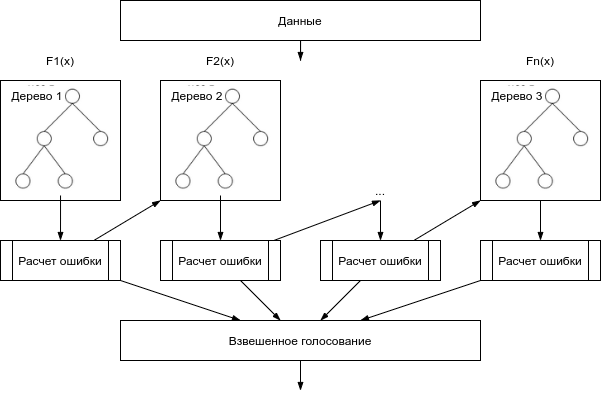
\includegraphics[scale=0.7]{Dissertation/images/DISSER-48.png}
    }
    \caption{Алгоритм построения бустинга }\label{fig:votesum}
\end{figure}


\subsection{Модель информационного обмена при проектировании системы поддержки принятия решения}\label{sec:ch2/sec3/sub3}
На рисунке ~\cref{fig:NNmodel} представлена работа блоков деревьев обработчиков классификатора. Все блоки взаимосвязанны друг с другом и образуют интеллектуальную модель поддержки принятия решений.
\begin{figure}[ht]
    \centerfloat{
        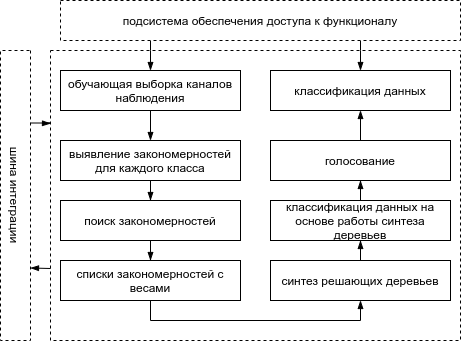
\includegraphics[scale = 0.8]{Dissertation/images/DISSER-1.png}
    }
    \caption{Работа блоков деревьев обработчиков классификатора}\label{fig:NNmodel}
\end{figure}

Основные блоки интеллектуального модуля поддержки принятия решений это:

\begin{enumerate}
    \item база объектов, описывающая параметры конфигурации типовых информационных систем,
    \item база знаний прецендентов, сформированная базой объектов,
    \item нечеткая база знаний из каналов наблюдений, формируемая на основе закономерностей, получаемых из обучающей выборки,
    \item нейронечеткий механизм, который обучается и формирует нечеткую функцию рекомендаций,
    \item блок адаптации данных, данный блок принимает на вход данные получаемые от пользовательских запросов к системе,
    \item блок обучения деревьев классификатора, где происходит обучение механизма выявления закономерностей,
    \item механизм поиска по прецендентам, где происходит обработка запросов и сопостовление процедента с предъявляемым параметром или каналом наблюдения.
\end{enumerate}

На рисунке ~\cref{fig:NNproc} представлена модель обработки данных в укрупненном масштабе. 
\begin{figure}[ht]
    \centerfloat{
        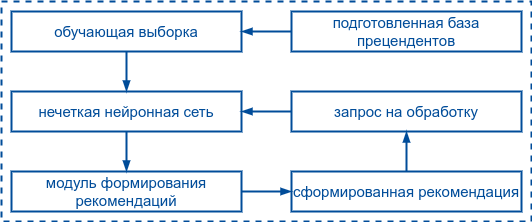
\includegraphics[scale=0.8]{Dissertation/images/DISSER-2.png}
    }
    \caption{Модель обработки данных }\label{fig:NNproc}
\end{figure}

Если рассматривать задачу с точки зрения теории управления, то мы получаем адаптивную комбинированную систему автоматизированного управления (т.к. обучение происходит с участием человека) с возмущением. 
Управляющая система представлена на рисунке ~\cref{fig:NNsau} в укрупненной абстракции. 
\begin{figure}[ht]
    \centerfloat{
        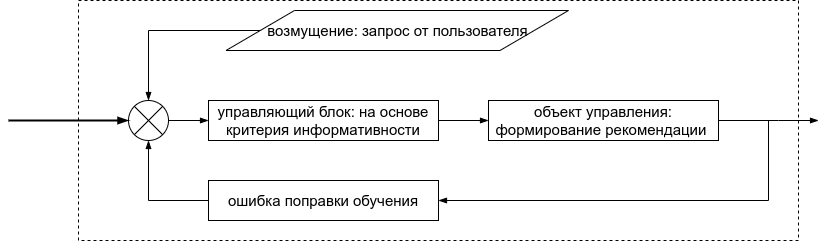
\includegraphics[scale=0.65]{Dissertation/images/DISSER-3.png}
    }
    \caption{Модель обработки данных }\label{fig:NNsau}
\end{figure}

Сравнительная таблица методов управления представлена на Рисунке ~\cref{fig:Csau}
\begin{figure}[ht]
    \centerfloat{
        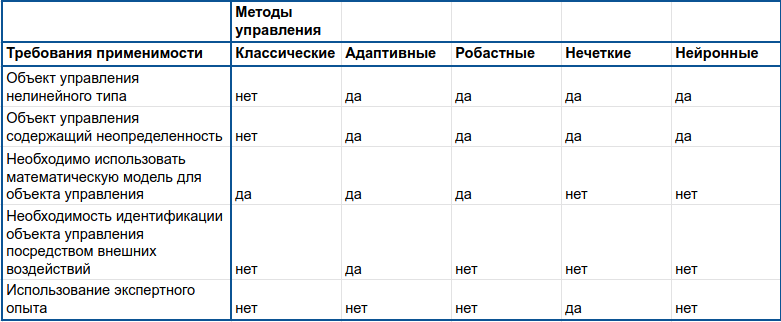
\includegraphics[scale=0.65]{Dissertation/images/DISSER-19.png}
    }
    \caption{Сравнительная таблица методов управления}\label{fig:Csau}
\end{figure}

Модель поддержки принятия решения может быть рассмотрена, как система автоматического управления с возмущением комбинированного типа. Входная информация поступает на линейный вход в модель обаботки информации и структуризации семантических данных ${z}$, обратная связь послупает от модуля расчета ошибки работы нейронной сети, здесь к управляющей системе возвращается информация о состоянии объекта управления ${у}$. Информация о состоянии объекта управления и возмущении ${w}$ поступает на вход к объекту управления, далее информация обрабатывается в соответствии с целью формирования рекомендаций, где объект управления получает воздействия от блока управления в виде набора рекомендаций и в виде управляющих воздействий передается на объект управления
\begin{equation}
    \label{eq:equation30}
    S = \{S_y, O_y, C,  \overrightarrow{z}, \overrightarrow{y}, \overrightarrow{w}\}
\end{equation}

Модель вычислений представлена в виде
\begin{equation}
    \label{eq:equation30}
    E_S=<K_B,F_B,R_B,I^e,R^e>
\end{equation}


где $K_B$- база знаний в виде закономерностей; 

$F_B$- таблица фактов $S$;

$R_B$- таблица закономерностей, создаваемая модулем интерпретатором в ходе вычислений, содержит информацию о причинах возникающих изменений в базе правил, а также поправки, комментарии, внесенные экспертом в базу знаний для объяснений; 

$R^e$ — отношения между объектами; 

$I^e$ — интерпретатор, который опирается на последовательное исполнение: $I^e =<I^{e1}, I^{e2}, I^{e3}, I^{e4}>$,

$I^{e1}$ - процесс выбора из базы знаний подмножества необходимых закономерностей; 

$I^{e2}$ - процесс сверки с прецендентами; 

$I^{e3}$ - процесс принятия оптимального решения; 

$I^{e4}$ — процесс отбора по критерию максимума взвешенной информативности.

Модель системы интеллектуального вывода может быть представлена следующим образом
\begin{equation}
    \label{eq:equation31}
    NN=<A_r,X,Y,M^n,E_d,I^{n1}, I^{n2} >,
\end{equation}

где $A_r$ — топология деревьев классификации на класс для принятия решений и вывода рекомендации; 

$X, У$ - множества входов и выходов для модуля обработки деревьев соответственно; 

$М^n$ — множество деревьев классификации; 

$E_d$ — обучающая и тестирующая выборки; 

$I^{n1}, I^{n2}$ — интерпретаторы обучения и вычислений деревьев принятия решений и формулирования рекомендаций.

Таким образом, интегрированная система деревьев  принятия решений для экспертного вывода модели вычислений будет иметь следующий вид
\begin{equation}
    \label{eq:equation32}
    NES=<K_B,X,Y,M^n,E_d,R_e, I^{n1}, I^{n2} >
\end{equation}

В экспертной системе с дереьвями принятия решений сохраняется база закономерностей экспертной системы, с помощью которой строится система экспертного вывода с некоторыми входами $X$ и выходами $Y$, где $E_d$ — обучающая и тестирующая выборки модели поддержки принятия решений;  $I^{n1}, I^{n2}$ — интерпретаторы проектируемые для обучения деревьев классификации, а также для формирования рекомендаций соответственно; новая система получает новый набор отношений между объектами в виде $R_e$.

Разработанная в работе модель экспертной системы с деревьями решений проектируется с целью формировать рекомендации. Для извлечений рекомендаций необходимо ввести данные о проектируемой системе согласно шаблону опроса, затем запустить модуль принятия решений. 
Модель вычислений с использованием методов конъюнкционной логики на основе прецедентов имеет следующий вид:

\begin{equation}
    \label{eq:equation33}
    PS=<K_{B1},K_{B2},A(p), I^p >
\end{equation}

где $K_{B1},K_{B2}$- блок прецедентов и блок знаний о проектированнии архитектуры; 

$А(р)$ — алгоритм, который определяет схожие прецеденты р.

Интерпретатор $І_р$, использующий алгоритм $А(р)$ и модуль $К_{В2}$, который обрабатывает данные, хранящиеся в базе знаний $К_{B2}$. Все это может быть представлена как совокупность процессов
\begin{equation}
    \label{eq:equation34}
    I^p = <I^{p1}, I^{p2}, I^{p3}, I^{p4}>
\end{equation}

где $I^{p1}$ - сохранение, 

$I^{p2}$ - обнаружение, 
$I^{p3}$ - адаптация , 
$I^{p4}$ - пересмотр

Гибкость модели обучения записит от следущих параметров

\begin{equation}
    \label{eq:equation35}
    NES^p=<K_B,X,Y,M^n,E_d,R_n, I^{np}, I^{n2}, I^p >
\end{equation}

Конъюнкционные правила сохраняются в виде $K_{B1}$, также в виде прецедентов $K_{B2}$ ; $R^n$ — отношения между объектами представляются в виде некоторого отношения вложенности или принадлежности (определяется семантическим интерпретатором логики). Поиск решений разбивается на решение получаемое с помощью аппроксимации нечеткой логики и работы по выявления прецендентов на основе работы деревьев поиска закономерностей на основе критерия максимума взвешенной информативности $І^р$ с действием алгоритма $А(р)$ определения похожих прецедентов. Обучение $І^р$ производится на основе данных из прецедентов из ТРИЗ графа, состоящего из каналов наблюдения.


\subsection{Алгоритм оценки устойчивости модели}\label{sec:ch2/sec3/sub4}

Рассмотрим следующую систему. Пусть система поддержки решений будет представлена в виде:
\begin{equation}
    \label{eq:equation46}
     \left\{\begin{array}{ll} 
    \dot{x} = X(x,t) \textrm{,} 
    \\ X(0,t) = 0 \textrm{,} 
     \forall{t} \geq t_0
      & \end{array} \right. \]
\end{equation}

Пусть отклик от обучения будет представлен в виде постоянного возмущения $R(x,t)$
\begin{equation}
    \label{eq:equation47}
    \dot{x} = X(x,t) + R(x,t),
\end{equation}

где $R(0,t) \neq 0$ и момент покоя $x = 0$ не является решением данного уравнения.

Положение системы, согласно \cite{Tau}, будет определено, как устойчивое при постоянно действующих возмущениях, если будет существовать такое малое $\varepsilon$ для которого найдутся такая пара положительных $\delta_0$ и $\delta_1$, что при выполнении неравенства $|R(x,t)| < \delta_1$ при всех $|x|\leq \varepsilon$ и $t \geq t_0$, движение возмущения может быть описано неравенством $|x(x^0, t)| < \varepsilon$ и $t \geq t_0$.
В общем смысле система поддержки решений на основе модуля поиска закономерностей при малых отклонениях обучения на экспоненциальную функцию потерь малы т.е. отклонение положения возмущения от невозмущенного положения малы. Определим меру возмущений, согласно теореме Малкина \cite{Tau}
\begin{equation}
    \label{eq:equation48}
    |grad V(x,t)| = \sqrt{\sum_{i=1}^n{\frac{\partial V}{\partial x_i}}^2} \leq N
\end{equation}

где $N$ - положительная константа.

Тогда, система принятий решений и интеллектуальный модуль должны быть ограничены в отклонениях в возмущениях в виде некоторой константы $N$. Таким образом, переобучение или недобучение системы определяются, как состояния, которые выходят за предел допустимого $N$ отклонений в возмущениях.

Выведем последовательность действий при обработке информации в модуле деревьев обработкии поиска закономерностей на основе нечеткого модуля продукционных правил. Представим перечень шагов:
\begin{enumerate}
    \item ввод данных в систему, система получает набор переменных, которые принимают конкретные значения в зависимости от значений введенных данных, данные передаются на вход, множество введенных данных обозначим как $P =\{p_1, p_2, ..., p_n\}$,
    \item сохраняем набор параметров в сущность, создаем сущность описание прецендента,
    \item определяем важности параметров, присваиваем весовые коэффициенты каждому параметру $W = \{W_1, W_2, ..., W_n\}$
    \item сохраняем размерность количества признаков, введеных в систему,
    \item переводим значения характеристик в числовые переменные посредством фукционалов принадлежности,
    \item передаем на обработку в дерево для поиска по таблице фактов,
    \item создаем сущность для агрегированная и обработка промежуточной информации, 
    \item проходим в цикле по всем закономерностям и сохраняем найденное в агрегированную сущность,
    \item в случае отсутствия данных создаем отдельную подсущность для хранения пустых множеств значений параметров переменных отображения, созданная подсущность будет помогать основному каналу наблюдения аппроксимировать данные черех обработку обратного обучения через деревья связи,
    \item в сущносте с отобранными по рангам соответствия всем значениям, проверяем на метрическую принадежность векторов признаков к вектору введенных переменных, используется критерий максимума взвешенной информативности, где прецедент, находящийся в обработке $A_j$ сравнивается с описанным вектором перенесенных запросом $P$, сравнения проходят согласно векторам весов важности в упорядоченном множестве,
    \item производим расчет максимума взвешенной информативности, 
    \item рассчитываем расстояния максимума взвешенной информативности для граничных объектов,
    \item расчитываем шаги сходства, степени возможного правдоподобия или близости $S(A,P) = \frac{(1-D)}{D_{max}}$, нормируем и приводим в долевое выражение от $\{0, ..., 1\}$,
    \item в случае, если не находятся похожие прецеденты , передаем запрос на уменьшение уровня правдоподобия и производим расчеты заново,
    \item в случае заполнения значений и отбору прецедентов не по всем переменным, сохраняем то состояние, что есть и выводим ответ,
    \item сформированный ответ сохраняем в конъюнкционную базу прецедентов для последующего использование.
\end{enumerate}

На Рисунке~\cref{fig:NN1} указано исполнения вышеописанных шагов 1-9, на Рисунке~\cref{fig:NN2} все остальные.
\begin{figure}[ht]
    \centerfloat{
        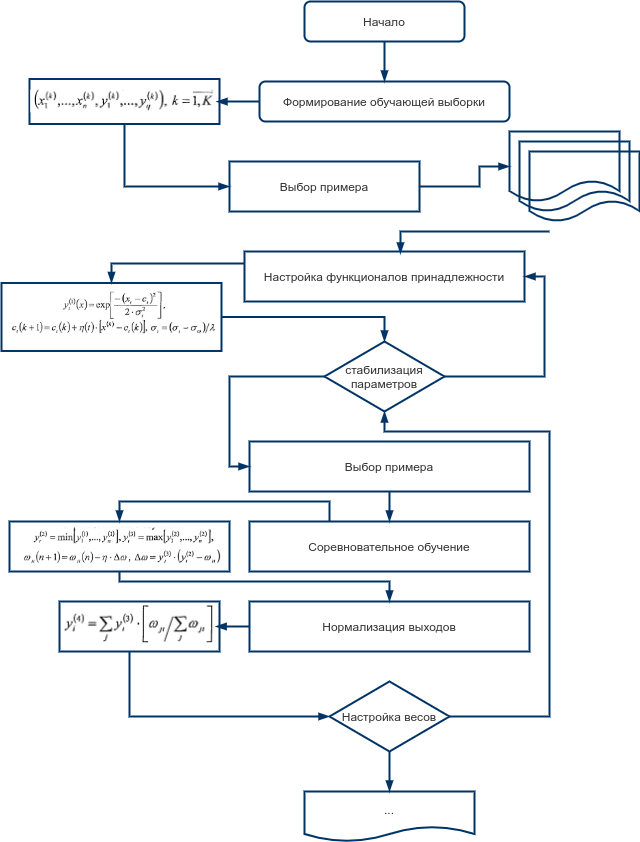
\includegraphics[scale=0.8]{Dissertation/images/DISSER-29.png}
    }
    \caption{Последовательность обработки данных в модуле обработки деревьями поиска закономерностей}\label{fig:NN1}
\end{figure}
\begin{figure}[ht]
    \centerfloat{
        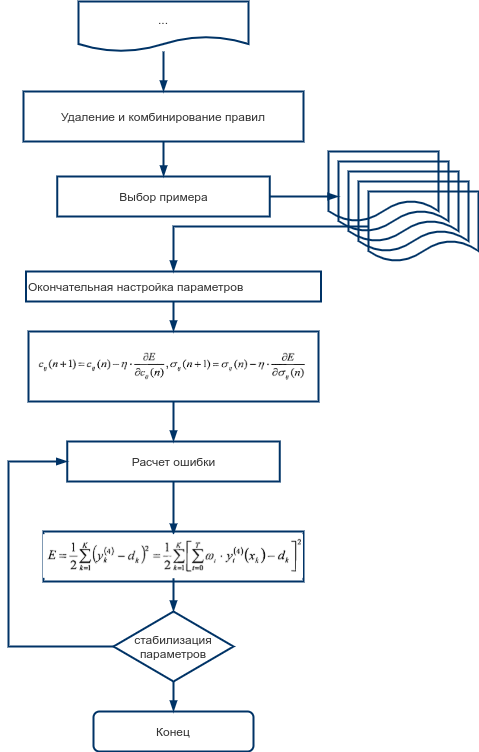
\includegraphics[scale=0.5]{Dissertation/images/DISSER-30.png}
    }
    \caption{Последовательность обработки данных в модуле классификатора и выбора рекомендаций}\label{fig:NN2}
\end{figure}



Пусть система проектирования представляется в виде положительно определенной функции $V(x,t)$, рассмотрим функцию $\omega_1(x)$, которая выступит ограничением $V(x,t) \geq \omega_1(x)$ на функцию работы системы
\begin{equation}
    \label{eq:equation49}
    m = min_{x \in S_{\varepsilon}}\omega_1(x)
\end{equation}

Представим область определения функции $V(x,t)$  в виде некоторой сферы $S_\varepsilon$ при всех $t \geq t_0$
\begin{equation}
    \label{eq:equation50}
    V(x,t) \geq \omega_1(x) \geq m
\end{equation}

Пусть обучение системы выражается как $\dot{V}(x,t)$ в соответствии с представлением ~\cref{eq:equation46} является отрицательной функцией. Тогда, определим положительную функцию $\omega_2(x)$
\begin{equation}
    \label{eq:equation50}
    \dot{V(x,t)} \leq -\omega_2(x) , t \geq t_0
\end{equation}

Таким образом, в силу того, что $\omega_2(x)$ положительно определена существует некоторое $h$, которое удовлетворит условие
\begin{equation}
    \label{eq:equation50}
    \dot{V(x,t)} \leq -\omega_2(x) < -h
\end{equation}

Выразим систему $\dot{V(x,t)}$ согласно ~\cref{eq:equation47} с некоторым возмущением 
\begin{equation}
    \label{eq:equation51}
    \dot{V(x,t)} = \frac{\partial V}{\partial t} + \sum_{i=1}^n{\frac{\partial V}{\partial x_i}}X_i + \sum_{i=1}^n{\frac{\partial V}{\partial x_i}}R_i = \dot{V} + \sum_{i=1}^n{\frac{\partial V}{\partial x_i}}R_i
\end{equation}

Согласно неравенству Коши-Шварца ~\cite{Korn}
\begin{equation}
    \label{eq:equation52}
    \sum^n_{i=1}{a_ib_i}^2 \leq \sum_{i=1}^n{a^2_i} \sum_{i=1}^n{b^2_i} 
\end{equation}

Получим
\begin{equation}
    \label{eq:equation53}
    |\sum_{i=1}^n{\frac{\partial V}{\partial x_i}}R_i| \leq {\sqrt {\sum_{i=1}^n{\frac{\partial V}{\partial x_i}}}}^2 {\sqrt{\sum_{i=1}^n{R_i}}^2} = |gradV(x,t)||R(x,t)|
\end{equation}

Находим
\begin{equation}
    \label{eq:equation54}
    \dot{V(x,t)} \leq \dot{V(x,t)} +  |\sum_{i=1}^n{\frac{\partial V}{\partial x_i}}R_i| < -h + N |R(x,t)|
\end{equation}

Допустим $|R(x,t)| < \delta_1 = h/(2N), |x| \leq \varepsilon, t \geq t_0$, тогда отклонение возмущения примет вид
\begin{equation}
    \label{eq:equation55}
    \dot{V(x,t)}  < -h/2
\end{equation}

Решение $x(x^0, t)$ при $|x^0|<\delta_0$ удовлетворит условию
\begin{equation}
    \label{eq:equation56}
    |x(x^0,t_0), t_0|  = V(x^0, t_0) < m
\end{equation}

В случае, если отклонение в возмущении будет возрастать и станет больше $m$, то система обучения станет неустойчивой. Для более подробного изучения устойчивости системы деревьев поддержки принятия решений с нечеткой логикой можно провести с помощью иных аналитических методов. Такая работа выходит за пределы темы исследования и может быть изучена читателем самостоятельно. Для систематизации методов анализа устойчивости моделей представлен Рисунок~\cref{fig:Trel}.

\begin{figure}[ht]
    \centerfloat{
        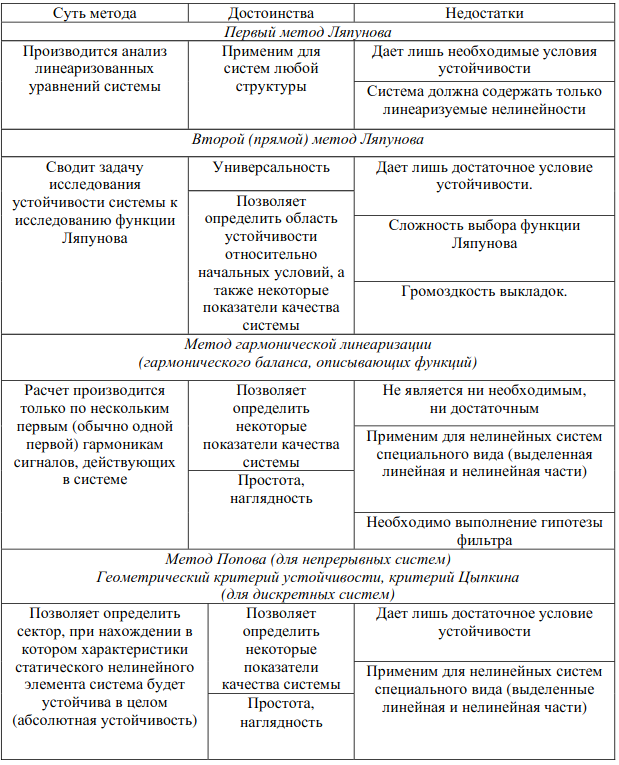
\includegraphics[scale=0.65]{Dissertation/images/DISSER-20.png}
    }
    \caption{Сравнительная таблица применения методов анализа устойчивости}\label{fig:Trel}
\end{figure}

Сравнительная таблица применения методов анализа устойчивости представлена на Рисунке~\cref{fig:Trel}.

\section{Выводы по главе}\label{sec:ch2/conc}

В данной главе решены следующие задачи:
\begin{enumerate}
    \item продемонстрирована математическая модель деревьев поддержки принятия решений и формулирования рекомендаций на основе нечеткого вывода Мамдани. Определены структура отображения входной и выходной информации, процесс обработки, фазификации и дефазификации наборов данных,
    \item разработан алгоритм модели поддержки принятия решений и формирования рекомендаций на основе прецедентов для задач принятия решений,
    \item продемонстрирована природа устойчивости обучения, рассмотренная, как отклонение в возмущениях в нелинейной адаптивной комбинированной системе с возмузением,
    \item продемонстрирована модель конъюнкционного вывода на основе нечетких функционалов принадлежности и работы деревьев поиска закономерностей,
    \item разработана модель формирования базы знаний, на основе таблицы ТРИЗ и семантического структурирования лексических термов, проведена работа по моделированию отображения графа в деревья закономерностей на основе аппроксимации эвристического отображения синтезом деревьев на основе критерия максимума взвешенной инофрмативности,
	\item проведен анализ конкурентных решений на рынке информационных технологий,
	\item систематизированы типы транзакционных моделей, 
	\item продемонстрирована постановка задачи проектирования архитектуры программного обеспечения, рассмотрены основные ограничения, допущения,
	\item продемонстрировано решение проблемы проектирования устойчивой архитетектуры автоматизированной системы управления,
	\item систематизирована информация по наиболее актуальным вопросам транзакционных проблем при проектировании архитектуры программного обеспечения автоматизированных систем управления.
\end{enumerate}

В результате каждая следующая закономерность стремится выделить наименее покрытые объекты, оказавшиеся наиболее трудными для предыдущих закономерностей. Это способствует повышению различности закономерностей, более равномерному покрытию объектов и повышению
обобщающей способности выпуклой комбинации закономерностей.

Перевыборка по отношению к выборке рассматривается как выборка по отношению к генеральной совокупности.
Важнейшим преимуществом бутстрапа являются:  
\begin{enumerate}
	\item простота реализации;  
	\item отсутствие необходимости гипотез о параметрах распределения данных;   
	\item возможность оценивания многих статистических характеристик (среднего, дисперсии, стандартного отклонения, доверительных интервалов, квантилей, коэффициентов корреляции и др.). 
\end{enumerate}

К недостатку метода можно отнести использование малореалистичного предположения о независимости перевыборок и значительные вычислительные затраты при их многократном построении. Метод оказывается особенно полезным, когда теоретическое распределение данных неизвестно или объем выборки мал для прямой статистической оценки.

\clearpage           % Глава 2
\chapter{Модель специального математического и алгоритмического обеспечения системы анализа, принятия решений и обработки информации в проектировании архитектуры автоматизированных систем управления}\label{ch:ch3}
\section{Основные понятия и определения}\label{sec:ch3/sec1}
Система искусственного интеллекта, которая обрабатывает слабоструктурированную и трудно формализуемую информацию в некоторой предметной области, может интерпретировать и объяснять методы решения задач принятия решения. Экспертные системы способны анализировать и предлагать множество решений на основе некоторых параметрических критериев. Такие системы обрабатывают информацию на основе некоторых формализованных структуированных продукционных правилах логического вывода, в данной работе модулем выявления продукционных правил выступает обработчик нечеткой логики.


Элементами экспертной системы являются следующие модули блоки обработчики:
\begin{enumerate}
    \item база знаний — некоторое семантическое представление знаний, формализованных в виде базы фактов,
    \item блок логического выводе — блок, который моделирует механизм продукционных правил на основе правил логического вывода,
    \item блок интерпретаций — блок, который интерпретирует некоторое семантическое представление получаемых системой данных,
    \item блок формирования рекомендаций — данный блок формирует рекомендации.
\end{enumerate}
Таким образом система поддержки принятия решения, основанные на экспертных систмах главным образом опираются на модуль формирования продукционных правил.

\section{Требования к модели поддержки принятия решений}\label{sec:ch3/sec2}
Требования для разработки системы поддержки принятия решений вырабатываются на основе анализа проблем в области задачи принятия решений. Например, для поддержки принятия решений в области проектирования программного обеспечения крайне сложно аализировать организацию шаблонов проектрования кода на уровне отношений между сущности, также довольно сложнореализуемой задачей является анализ индексации таблиц и определения внешний и составных ключей, отношений между таблицами в БД.
Таким образом, основными требованиями при разработке модели поддержки принятия решений выступили требования по формированию вектора рекомендаций для проектирования того или иного набора инструментов для реализации задач проектирования. Для решения такой задач, после проведения анализа проблематики и выявления альтернатив, была разработана модель нйеронной сети на основе нечеткой логики. Требования к модели принятия решений блоком нейронной сети, главным образом, определялся возможностью реализации продукционного вывода на основе базы знаний, но с возможностью обновления и адаптации под пользовательские запросы. Система должна уметь адаптироваться под запросы пользователей, а также адаптировать свою семантическую продукционную структуру дополняя базу новыми фактами, новыми прецендентами.
Основные требования при проектирования модели поддержки принятия решений перечислены здесь:
\begin{enumerate}
	\item система должна уметь интерпретировать слабоструктурированный текст в семантически верное продукционное правило,
	\item система должна уметь выявлять эвристические закономерности и аппроксимировать функционал оптимизации подбора рекомендаций,
	\item система должна уметь выявлять продукцоинные правила,
	\item система должна уметь обрабатывать отношения между объектами,
	\item система должна уметь формировать рекомендацию.
\end{enumerate}


\subsection{Модель информационного обмена при проектировании системы поддержки прнятия решения}\label{sec:ch3/sec2/sub1}
На рисунке ~\cref{fig:NNmodel} представлена работа блоков обработчиков нейронной сети. Все блоки взаимосвязаннеы друг с другом и образуют интеллектуальную модель поддержки принятия решений.
\begin{figure}[ht]
    \centerfloat{
        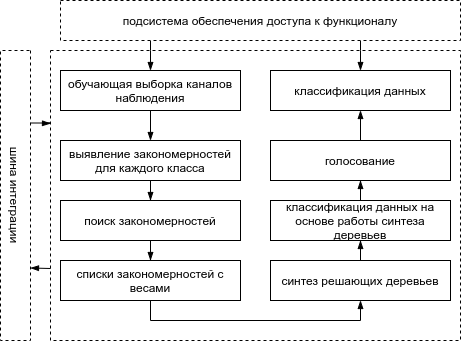
\includegraphics[scale=0.8]{Dissertation/images/DISSER-1.png}
    }
    \caption{Модель нейронной сети}\label{fig:NNmodel}
\end{figure}

Основные блоки интеллектуального модуля поддержки принятия решений это:
\begin{enumerate}
\item база объектов, описывающая параметры конфигурации типовых информационных систем,
\item база знаний прецендентов, сформированная базой объектов,
\item продукционная нечеткая база знаний, формируемая на основе фактов и правил продукционного формирования правил, получаемых из базы знаний,
\item нейронечеткий механизм, который обучается и формирует  нечеткую функцию рекомендаций,
\item блок адаптации данных, данный блок принимает на вход данные получаемые от пользовательских запросов к системе,
\item блок обучения нейронной сети, где происходит обучение нейросетевого механизма,
\item механизм поиска по прецендентам, где происходит обработка запросов и сопостовление процедента с предъявляемым параметром.
\end{enumerate}

На рисунке ~\cref{fig:NNproc} представлена модель обработки данных нейросетевой моделью в укрупненном масштабе. 
\begin{figure}[ht]
    \centerfloat{
        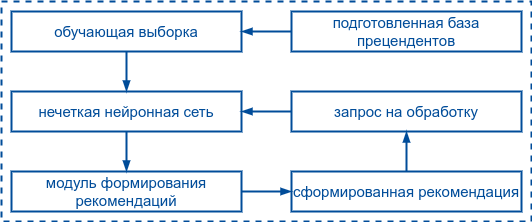
\includegraphics[scale=0.8]{Dissertation/images/DISSER-2.png}
    }
    \caption{Модель нейронной сети}\label{fig:NNproc}
\end{figure}

Если рассматривать задачу с точки зрения теории управления, то мы получаем адаптивную комбинированную систему автоматизированного управления (т.к. обучение происходит с участием человека) с возмущением. 
Управляющая система представлена на рисунке ~\cref{fig:NNsau} в укрупненной абстракции. 
\begin{figure}[ht]
    \centerfloat{
        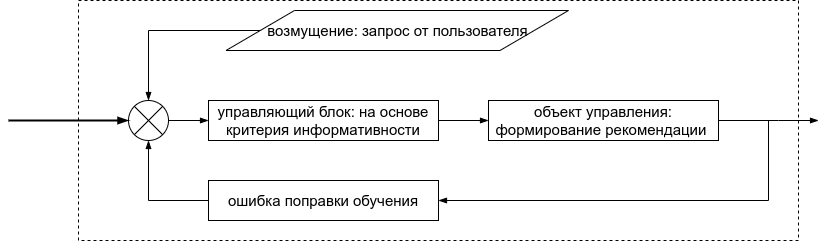
\includegraphics[scale=0.5]{Dissertation/images/DISSER-3.png}
    }
    \caption{Модель нейронной сети}\label{fig:NNsau}
\end{figure}

Сравнительная таблица методов управления представлена на Рисунке ~\cref{fig:Csau}
\begin{figure}[ht]
    \centerfloat{
        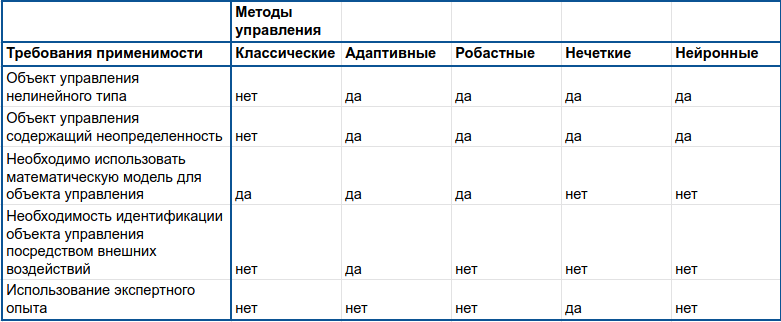
\includegraphics[scale=0.65]{Dissertation/images/DISSER-19.png}
    }
    \caption{Сравнительная таблица методов управления}\label{fig:Csau}
\end{figure}

Модель поддержки принятия решения может быть рассмотрена, как система автоматического управления с возмущением комбинированного типа. Входная информация поступает на линейный вход в модель обаботки информации и структуризации семантических данных ${z}$, обратная связь послупает от модуля расчета ошибки работы нейронной сети, здесь к управляющей системе возвращается информация о состоянии объекта управления ${у}$. Информация о состоянии объекта управления и возмущении ${w}$ поступает на вход к объекту управления, далее информация обрабатывается в соответствии с целью формирования рекомендаций, где объект управления получает воздействия от блока управления в виде набора рекомендаций и в виде управляющих воздействий передается на объект управления
\begin{equation}
    \label{eq:equation30}
    S = \{S_y, O_y, C,  \overrightarrow{z}, \overrightarrow{y}, \overrightarrow{w}\}
\end{equation}

Модель вычислений представлена в виде
\begin{equation}
    \label{eq:equation30}
    E_S=<K_B,F_B,R_B,I^e,R^e>
\end{equation}


где $K_B$- база знаний в виде продукционных правил; 

$F_B$- таблица фактов $S$;

$R_B$- таблица продукционных выводов, создаваемая модулем интерпретатором в ходе вычислений, содержит информацию о причинах возникающих изменений в базе правил, а также поправки, комментарии, внесенные экспертом в базу знаний для объяснений; 

$R^e$ — отношения между объектами; 

$I^e$ — интерпретатор, который опирается на последовательное исполнение: $I^e =<I^{e1}, I^{e2}, I^{e3}, I^{e4}>$,

$I^{e1}$ - процесс выбора из базы знаний подмножества необходимых продукицонных правил; 

$I^{e2}$ - процесс сверки с прецендентами; 

$I^{e3}$ - процесс принятия оптимального решения; 

$I^{e4}$ — процесс исполнения правила.

Модель системы интеллектуального вывода может быть представлена следующим образом
\begin{equation}
    \label{eq:equation31}
    NN=<A_r,X,Y,M^n,E_d,I^{n1}, I^{n2} >,
\end{equation}

где $A_r$ — топология нейронной сети; 

$X, У$ - множества входов и выходов нейронной сети соответственно; 

$М^n$ — множество искусственных нейронов; 

$E_d$ — обучающая и тестирующая выборки; 

$I^{n1}, I^{n2}$ — интерпретаторы обучения и вычислений нейронной сети.

Таким образом, интегрированная нейронная сети для экспертного вывода модели вычислений будет иметь следующий вид
\begin{equation}
    \label{eq:equation32}
    NES=<K_B,X,Y,M^n,E_d,R_e, I^{n1}, I^{n2} >
\end{equation}

В экспертной системе с нейронной сетью сохраняется база правил экспертной системы, с помощью которой строится нейронная сети с некоторыми входами $X$ и выходами $Y$, где $E_d$ — обучающая и тестирующая выорки нейронной сети;  $I^{n1}, I^{n2}$ — интерпретаторы проектируемые для обучения нейронной сети, а также для формирования рекомендаций соответственно; новая система получает новый набор отношений между объектами в виде $R_e$.

Разработанная в работе модель экспертной системы с нейронной сетью проектируется с целью формировать реккомендации. Для извлечений рекомендаций необходимо ввести данные о проектируемой системе согласно шаблону опроса, затем запустить модуль принятия решений. 
Модель вычислений с использованием методов продукционной логики на основе прецедентов имеет следующий вид
\begin{equation}
    \label{eq:equation33}
    PS=<K_{B1},K_{B2},A(p), I^p >
\end{equation}

где $K_{B1},K_{B2}$- блок прецедентов и блок знаний о проектированнии архитектуры; 

$А(р)$ — алгоритм, который определяет схожие прецеденты р.

Интерпретатор $І_р$, использующий алгоритм $А(р)$ и модуль $К_{В2}$, который обрабатывает данные, хранящиеся в базе знаний $К_{B2}$. Все это может быть представлена как совокупность процессов
\begin{equation}
    \label{eq:equation34}
    I^p = <I^{p1}, I^{p2}, I^{p3}, I^{p4}>
\end{equation}

где $I^{p1}$ - сохранение, 

$I^{p2}$ - обнаружение, 
$I^{p3}$ - адаптация , 
$I^{p4}$ - пересмотр

Гибкость модели обучения записит от следущих параметров

\begin{equation}
    \label{eq:equation35}
    NES^p=<K_B,X,Y,M^n,E_d,R_n, I^{np}, I^{n2}, I^p >
\end{equation}

Продукционные правила сохраняются в виде $K_{B1}$, также в виде прецедентов $K_{B2}$ ; $R^n$ — отношения между объектами представляются в виде некоторого отношения вложенности или принадлежности (определяется семантическим интерпретатором логики). Поиск решений разбивается на решение полуаемое с помощью аппроксимации нечеткой логики и работы по выявления прецендентов на основе работы нейронной сети $І^р$ с действием алгоритма $А(р)$ определения похожих прецедентов. Обучение $І^р$ производится на основе данных из прецедентов, также на основе дополнений новыми знаниями от авторизованных пользователей экспертов.


\subsection{Модель принятия решений в модуле поддержки принятия решений}\label{sec:ch3/sec2/sub2}

Представим модель в виде некоторой нелинейной системы:
\begin{equation}
    \label{eq:equation36}
    \[ \varphi(y(x)) = \left\{\begin{array}{ll} x_i, i   = 0,1, ...,  n,\textrm{,}\\ y_k = f_y(x_1,x_2,...,x_n), k = 1,2,...,q & \end{array} \right. \]
\end{equation}

Представим множество возможных значений в следующем виде:
\begin{equation}
    \label{eq:equation37}
    U = \{u_j, u_{j+1},.., u_m\}
\end{equation}

где $u_j$ - оценка, которая проставляется в соответсвии с входной информацией в систему,

$m$ - мощность множества.

Решением задачи будет составление такого множества значений $Y*= \{y_1^*, y_2^*, ..., y_n^*\}$ на постившее множество $X* = \{x_1^*, x_2^*,...,x_n^*\}$. Таким образом, на множество, поступающих значений $X*$ формируется множство выходных значений $Y*$.
Для установления зависимости между объектами выразим эвристическую закономерность в виде обработки семантических лингвистических переменных. Для этого выразим объекты через некоторые терм множества:
\begin{equation}
    \label{eq:equation38}
    A = \{a_j, a_{j+1}, ..., a_m\}
\end{equation}
Данные семантические терм определяются на основе соотношения
\begin{equation}
    \label{eq:equation38}
    a_j = \sum_{p=1}^l\frac{\mu^{a_{j}(u^p_j)}}{u^p_j}
\end{equation}

$\mu^{a_{j}(u^p_j)}$ - степень принадлежности,

$u^p_j$ - объект принадлежности.

Степень принадлежности определяется на основе рангов принадлежности и определяется на основе соотношений следующей системы:
\begin{equation}
    \label{eq:equation40}
    \[ R(\mu) = \left\{\begin{array}{ll} \frac{\mu_1}{\r_1} = \frac{\mu_2}{\r_2} = ... = \frac{\mu_m}{\r_m}, i   = 0,1, ...,  m,\textrm{,}\\ \sum_{i=1}^m{\mu_i} = 1  & \end{array} \right. \]
\end{equation}
В соответствии с нормировкой находим:
\begin{equation}
    \label{eq:equation41}
    \[ R(\mu) = 
    \left\{\begin{array}{ll} 
    \mu_{n-1} = (1 + \frac{r_n}{r_{n-1}} + \frac{r_{n+1}}{r_{n-1}} + ... )^{-1} \textrm{,} 
    \\ \mu_{n+m} = (\frac{r_{n-1}}{r_n} + \frac{r_{n+1}}{r_n} + ... )^{-1}  & \end{array} \right. \]
\end{equation}

Получаемая матрица обладает следующими свойствами:
\begin{enumerate}
    \item транзитивность,
    \item симметричность,
    \item диагональность.
\end{enumerate}

На основании этих свойств выведем соотношение:
\begin{equation}
    \label{eq:equation42}
    s_{ij} = \frac{s_{kj}}{s_{ki}}
\end{equation}

На основе матрицы парных рангов составляется соотношение со значениями 9-ти бальной шкалы Саати 
На рисунке ~\cref{fig:ST} представлена 9-ти бальная шкала Саати.
\begin{figure}[ht]
    \centerfloat{
        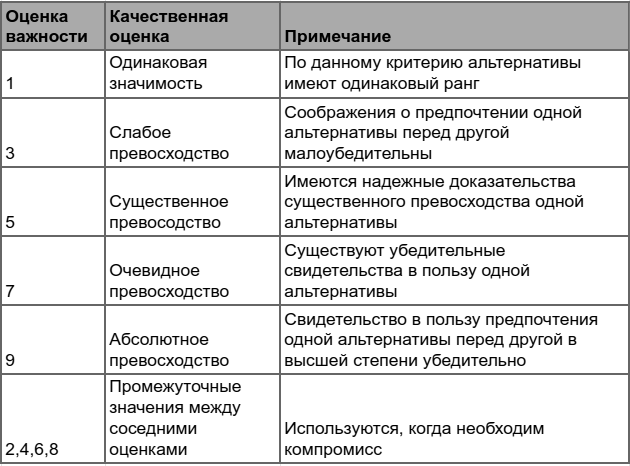
\includegraphics[scale=0.59]{Dissertation/images/APP-1.png}
    }
    \caption{9-ти бальная шкала Саати}\label{fig:ST}
\end{figure}

Приведем перечень функций принадлежности классов. Функция принадлежности к некоторому классу $s$ приведена в ~\cref{eq:equation43}.
\begin{equation}
    \label{eq:equation43}
    s(x,a,b,c) = \left\{\begin{array}{ll} 
    0, x\leq{a} \textrm{,} 
    \\ 2{\frac{x-a}{c-a}}^2, a\leq x\leq b    \\
    1 - 2{\frac{x-c}{c-a}}^2, b\leq x\leq c   \\ 
    1, x\geq c & \end{array} \right. \]
\end{equation}

где $b = \frac{a+c}{2}$.

Продукционное правило интерпретируется на основе:
\begin{equation}
    \label{eq:equation44}
    (i): Q ; P; A \rightarrow B;S,F,N
\end{equation}

где $(i)$ - имя нечеткого правила,

$Q$ - домен нечеткого правила,

$P$ - условия принятия, критерий принятия,

$A \ rightarrow B$ = ядро нечеткого продукционного правила,

$B$ - результирующее заключение, следствие,

$\rightarrow$ - знак продукционной секвенции,

$S$ - метод определения количественной истинности,

$F$ - коэффициент истины,

$N$ - ограничения продукционного вывода.


База знаний в соответствии с представление в виде продукционных правил образует совокупность множество, представимое в некоторой совокупности таблиц фактов.
Термы множества задаются с стандартной форме в виде логических отношений. База знаний задается в виде набора полей, объединенных некоторым логическим отношением, записанных в некоторой таблице совокупности фактов, на основании которых выводится продукционное правило.
Нечеткая база знаний может быть представлена в следующей виде в виде функции Мамдани

\begin{equation}
    \label{eq:equation45}
    \bigcup_{p=1}^{t_k} [\bigcap_{i=1}^{n} \(x_i = a_j^{kp}\)]   \rightarrow  \bigcup_{p=1}^{t_k} [ \bigcap_{k=1}^{q} \(y_k = b_j^{kp}\)  ]
\end{equation}

где  $j = {1,2, ..., q}$, $k = {1,2, ..., q}$, $p = {1,2, ..., t_k}$

База знаний формируется в соответствии с Рисунком ~\cref{fig:KBase}. Структура матрицы знаний представлена с Рисунком ~\cref{fig:ST}.
\begin{figure}[ht]
    \centerfloat{
        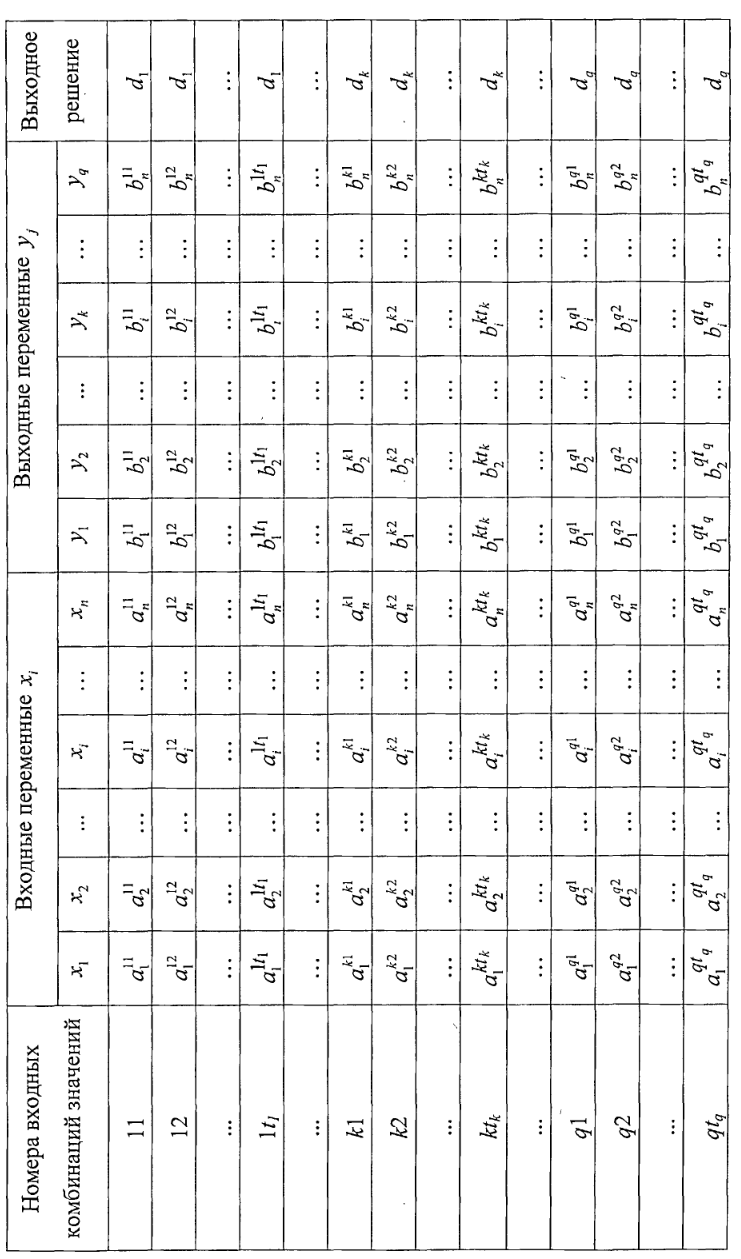
\includegraphics[scale=0.5]{Dissertation/images/DISSER-7.png}
    }
    \caption{Структура матрицы знаний}\label{fig:KBase}
\end{figure}


\subsection{Алгоритм оценки устойчивости специального математического и алгоритмического обеспечения проектирования архитектуры}\label{sec:ch3/sec2/sub3}
Рассмотрим следующую систему. Пусть система поддержки решений будет представлена в виде:
\begin{equation}
    \label{eq:equation46}
     \left\{\begin{array}{ll} 
    \dot{x} = X(x,t) \textrm{,} 
    \\ X(0,t) = 0 \textrm{,} 
     \forall{t} \geq t_0
      & \end{array} \right. \]
\end{equation}


Пусть отклик от обучения будет представлен в виде постоянного возмущения $R(x,t)$
\begin{equation}
    \label{eq:equation47}
    \dot{x} = X(x,t) + R(x,t)
\end{equation}

где $R(0,t) \neq 0$ и момент покоя $x = 0$ не является решением данного уравнения.

Положение системы, согласно \cite{Tau}, будет определено, как устойчивое при постоянно действующих возмущениях, если будет существовать такое малое $\varepsilon$ для которого найдутся такая пара положительных $\delta_0$ и $\delta_1$, что при выполнении неравенства $|R(x,t)| < \delta_1$ при всех $|x|\leq \varepsilon$ и $t \geq t_0$, движение возмущения может быть описано неравенством $|x(x^0, t)| < \varepsilon$ и $t \geq t_0$.
В общем смысле система поддержки решений на основе модуля нейронной сети при малых отклонениях обучения на нейронную сеть малы т.е. отклонение положения возмущения от невозмущенного положения малы. Определим меру возмущений, согласно теореме Малкина \cite{Tau}
\begin{equation}
    \label{eq:equation48}
    |grad V(x,t)| = \sqrt{\sum_{i=1}^n{\frac{\partial V}{\partial x_i}}^2} \leq N
\end{equation}

где $N$ - положительная константа.

Тогда, система принятий решений и интеллектуальный модуль должны быть ограничены в отклонениях в возмущениях в виде некоторой константы $N$. Таким образом, переобучение или недобучение системы определяются, как состояния, которые выходят за предел допустимого $N$ отклонений в возмущениях.

Выведем последовательность действий при обработке информации в модулей нейронной сети на основе нечеткого модуля продукционных правил. Представим перечень шагов:
\begin{enumerate}
    \item ввод данных в систему, система получает набор переменных, которые принимают конкретные значения в зависимости от значений введенных данных, данные передаются на вход, множество введенных данных обозначим как $P =\{p_1, p_2, ..., p_n\}$,
    \item сохраняем набор параметров в сущность, создаем сущность описание прецендента,
    \item определяем важности параметров, присваиваем весовые коэффициенты каждому параметру $W = \{W_1, W_2, ..., W_n\}$
    \item сохраняем размерность количества признаков, введеных в систему,
    \item переводим значения характеристик в числовые переменные посредством фукционалов принадлежности,
    \item передаем на обработку в нейронную сеть для поиска по таблице фактов,
    \item создаем сущность для агрегированная и обработка промежуточной информации, 
    \item проходим в цикле по всем продукционным правилам и сохраняем найденное в агрегированную сущность,
    \item в случае отсутствия данных создаем отдельную подсущность для хранения пустых множеств значений параметров переменных отображения, жанная подсущность будет помогать основному каналу наблюдения аппроксимировать данные черех обработку обратного обучения черех нейронные связи,
    \item в сущносте с отобранными по рангам соответствия всем значениям, проверяем на метрическую приналдежность векторов признаков к вектору введенных переменных, используется евклидова метрика $D(P,A_j) = \sqrt{\sum_{i=1}^n{a_i - p_i}^2w_i}$, где прецедент, находящийся в обработке $A_j$ сравнивается с описанным вектором пересенных запросом $P$, сравнения проходят согласно векторам важности в упорядоченном множестве,
    \item производим расчет евклидовой метрики расстояния $D$, 
    \item рассчитываем расстояния для граничных объектов $D_{max}(P) = \sqrt{\sum_{i=1}^n{p_{max} - p_{min}}^2w_i}$,
    \item расчитываем шаги сходства, степени возможного правдоподобия или близости $S(A,P) = \frac{(1-D)}{D_{max}}$, нормируем и приводим в долевое выражение от $\{0, ..., 1\}$,
    \item в случае, если не находятся похожие прецеденты , передаем запрос на уменьшение уровня правдоподобия и производим расчеты заново,
    \item в случае заполнения значений и отбору прецедентов не по всем переменным, сохраняем то состояние, что есть и выводим ответ,
    \item сформированный ответ сохраняем в продукционную базу прецедентов для последующего использование.
\end{enumerate}

На Рисунке~\cref{fig:NN1} указано исполнения вышеописанных шагов 1-9, на Рисунке~\cref{fig:NN2} все остальные.
\begin{figure}[ht]
    \centerfloat{
        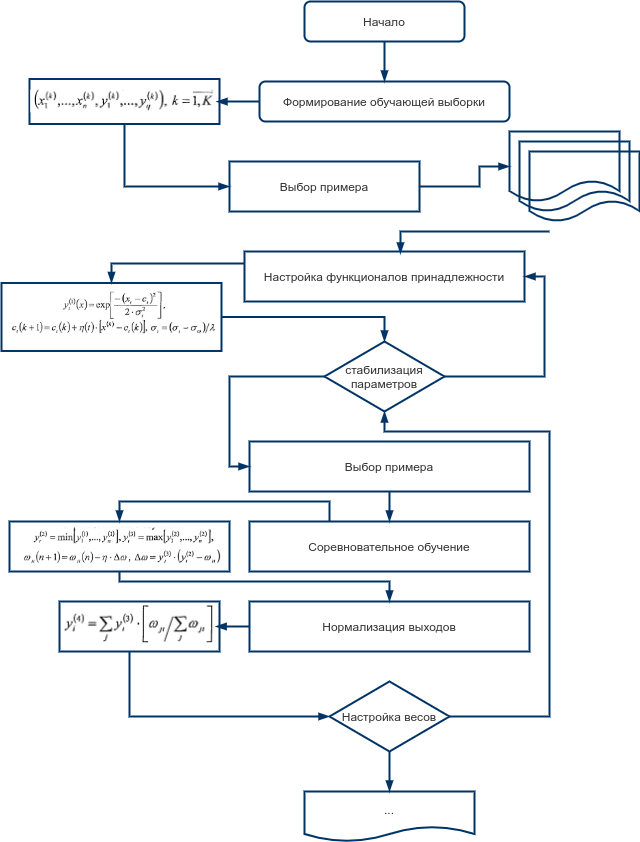
\includegraphics[scale=0.65]{Dissertation/images/DISSER-29.png}
    }
    \caption{Последовательность обработки данных в модуле нейронной сети}\label{fig:NN1}
\end{figure}
\begin{figure}[ht]
    \centerfloat{
        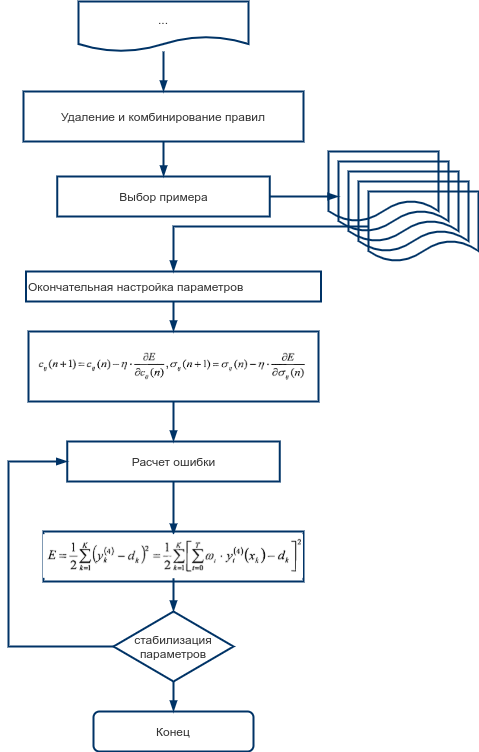
\includegraphics[scale=0.65]{Dissertation/images/DISSER-30.png}
    }
    \caption{Последовательность обработки данных в модуле нейронной сети}\label{fig:NN2}
\end{figure}



\subsection{Математическая модель системы проектирования устойчивой архитектуры программного обеспечения}\label{sec:ch2/sec3/sub1}
Пусть система проектирования представляется в виде положительно определенной функции $V(x,t)$, рассмотрим функцию $\omega_1(x)$, которая выступит ограничением $V(x,t) \geq \omega_1(x)$на функцию работы системы
\begin{equation}
    \label{eq:equation49}
    m = min_{x \in S_{\varepsilon}}\omega_1(x)
\end{equation}

Представим область определения функции $V(x,t)$  в виде некоторой сферы $S_\varepsilon$ при всех $t \geq t_0$
\begin{equation}
    \label{eq:equation50}
    V(x,t) \geq \omega_1(x) \geq m
\end{equation}

Пусть обучение системы выражается как $\dot{V}(x,t)$ в соответствии с представлением ~\cref{eq:equation46} является отрицательной функцией. Тогда, определим положительную функцию $\omega_2(x)$
\begin{equation}
    \label{eq:equation50}
    \dot{V(x,t)} \leq -\omega_2(x) , t \geq t_0
\end{equation}

Таким образом, в силу того, что $\omega_2(x)$ положительно определена существует некоторое $h$, которое удовлетворит условие
\begin{equation}
    \label{eq:equation50}
    \dot{V(x,t)} \leq -\omega_2(x) < -h
\end{equation}

Выразим систему $\dot{V(x,t)}$ согласно ~\cref{eq:equation47} с некоторым возмущением 
\begin{equation}
    \label{eq:equation51}
    \dot{V(x,t)} = \frac{\partial V}{\partial t} + \sum_{i=1}^n{\frac{\partial V}{\partial x_i}}X_i + \sum_{i=1}^n{\frac{\partial V}{\partial x_i}}R_i = \dot{V} + \sum_{i=1}^n{\frac{\partial V}{\partial x_i}}R_i
\end{equation}

Согласно неравенству Коши-Шварца ~\cite{Korn}
\begin{equation}
    \label{eq:equation52}
    \sum^n_{i=1}{a_ib_i}^2 \leq \sum_{i=1}^n{a^2_i} \sum_{i=1}^n{b^2_i} 
\end{equation}

Получим
\begin{equation}
    \label{eq:equation53}
    |\sum_{i=1}^n{\frac{\partial V}{\partial x_i}}R_i| \leq {\sqrt {\sum_{i=1}^n{\frac{\partial V}{\partial x_i}}}}^2 {\sqrt{\sum_{i=1}^n{R_i}}^2} = |gradV(x,t)||R(x,t)|
\end{equation}

Находим
\begin{equation}
    \label{eq:equation54}
    \dot{V(x,t)} \leq \dot{V(x,t)} +  |\sum_{i=1}^n{\frac{\partial V}{\partial x_i}}R_i| < -h + N |R(x,t)|
\end{equation}

Допустим $|R(x,t)| < \delta_1 = h/(2N), |x| \leq \varepsilon, t \geq t_0$, тогда отклонение возмущения примет вид
\begin{equation}
    \label{eq:equation55}
    \dot{V(x,t)}  < -h/2
\end{equation}

Решение $x(x^0, t)$ при $|x^0|<\delta_0$ удовлетворит условию
\begin{equation}
    \label{eq:equation56}
    |x(x^0,t_0), t_0|  = V(x^0, t_0) < m
\end{equation}

В случае, если отклонение в возмущении будет возрастать и станет больше $m$, то система обучения станет неустойчивой. Для более подробного изучения устойчивости системы нейронной сети с нечеткой логикой можно провести с помощью иных аналитических методов. Такая работа выходит за пределы темы исследования и может быть изучена читателем самостоятельно. Для систематизации методов анализа устойчивости моделей представлен Рисунок~\cref{fig:Trel}.

\begin{figure}[ht]
    \centerfloat{
        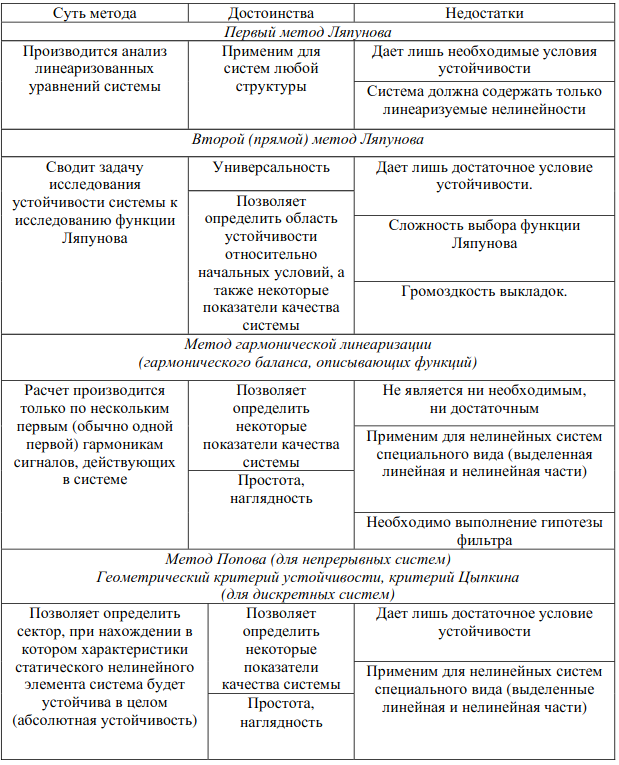
\includegraphics[scale=0.65]{Dissertation/images/DISSER-20.png}
    }
    \caption{Сравнительная таблица применения методов анализа устойчивости}\label{fig:Trel}
\end{figure}

Сравнительная таблица применения методов анализа устойчивости представлена на Рисунке~\cref{fig:Trel}.
\section{Выводы по главе}\label{sec:ch3/conc}
В данной главе решены следующие задачи:
\begin{enumerate}
    \item продемонстрирована математическая модель нейронной сети на основе нечеткого вывода Мамдани. Определены структура отображения входной и выходной информации, процесс обработки, фазификации и дефазификации наборов данных,
    \item разработан алгоритм нейронной сети на основе прецедентов для задач принятия решений,
    \item продемонстрирована природа устойчивости обучения, рассмотренная, как отклонение в возмущениях в нелинейной адаптивной комбинированной системе с возмузением,
    \item продемонстрирована модель продукционного вывода на основе нечетких функционалов принадлежности,
    \item разработана модель формирования базы знаний, на основе таблицы фактов и семантического структурирования лексических термов, проведена работа по моделированию отображения фактов в логические продукционные правила на основе аппроксимации эвристического отображения градиентом.
\end{enumerate}
\clearpage
           % Глава 3

\clearpage
           % Глава 4


\clearpage           % Глава 5
\chapter{Алгоритм оценки устойчивости специального математического и алгоритмического обеспечения проектирования архитектуры высоконагруженной информационной системы}\label{ch:ch6}

\section{Основные понятия и определения}\label{sec:ch6/sect1}
\section{Проблемы обеспечения устойчивости к внешним воздействиям и пути их решения}\label{sec:ch6/sect2}

\subsection{Общая характеристика проблем обеспечения устойчивости к внешним условиям}\label{subsec:ch6/sect2/sub1}
\subsection{Основные положения алгоритмического аппарата оценки устойчивости к внешним воздействиям}\label{subsec:ch6/sect2/sub2}
\subsection{Ограничения и допущения модели оценки устойчивости}\label{subsec:ch6/sect2/sub3}

\section{Алгоритм оценки устойчивости к внешним воздействиям}\label{sec:ch6/sect3}
\section{Методология оценки влияния человеческого фактора на функционирование специального математического и алгоритмического обеспечения проектирования архитектуры высоконагруженной информационной системы}\label{sec:ch6/sect4}
\subsection{Основные понятия и определения}\label{subsec:ch6/sect4/sub1}
\subsection{Математическая модель оценки влияния человеческого фактора на безошибочное функционирование}\label{subsec:ch6/sect4/sub1}
\subsection{Алгоритм оценки влияния человеческого фактора на устойчивость функицонирования}\label{subsec:ch6/sect4/sub1}
\subsection{Методологический подход к оценке влияния человеческого фактора на устойчивость функионирвования при отсутствии точных статистических данных}\label{subsec:ch6/sect4/sub1}
\section{Выводы по главе}\label{sec:ch6/sect3}


\clearpage           % Глава 6
 
\chapter*{Заключение}                       % Заголовок
\addcontentsline{toc}{chapter}{Заключение}  % Добавляем его в оглавление

%% Согласно ГОСТ Р 7.0.11-2011:
%% 5.3.3 В заключении диссертации излагают итоги выполненного исследования, рекомендации, перспективы дальнейшей разработки темы.
%% 9.2.3 В заключении автореферата диссертации излагают итоги данного исследования, рекомендации и перспективы дальнейшей разработки темы.
%% Поэтому имеет смысл сделать эту часть общей и загрузить из одного файла в автореферат и в диссертацию:

Разработана модель интеллектуального архитектурного проектирования и структурного проектирования человеко-машинных систем, предназначенных для автоматизации производства и интеллектуального обеспечения процессов управления и необходимой обработки данных в организационно-технологических и распределенных системах управления в различных сферах технологического производства и других областях человеческой деятельности .Представлена модель рекомендательной системы для проектирования различных типов архитектуры информационных систем, разработанная на основе нейронной сети и нечеткого продукционной декомпозиции. Метод имеет ряд преимуществ и недостатков. Поскольку отдельные системы рекомендаций на основе декомпозиции могут давать переменные результаты, потенциал для реализации таких моделей заключается в разнообразии предлагаемых рекомендаций. Модель обучается автоматически, т.е. модель обрабатывает данные и сама идентифицирует продукционные правила по представленным характеристикам на основе представленных знаний о типах архитектур для разных типов информационных систем, что является преимуществом для генерации знаний за счет возможность автоматизированного масштабирования базы знаний, недостатком является сложность формализации семантических и лингвистических термов на этапе выявления отношений между сущностями для проектирования организации кода и отношений между сущностями базы данных.

Основные результаты работы заключаются в следующем:
\begin{enumerate}
	\item проанализированы конкурентные решения на рынке,
	\item разработана модель проеткирования автоматизированных систем управоления на основе системы поддержки принятия решения,
	\item разработана методология поддержки принятия решений при проеткировании архитектуры программного обеспечения,
	\item разработана математическая модель системы поддержки принятия решений для проектирования автоматизированных систем управления.
\end{enumerate}
%% Согласно ГОСТ Р 7.0.11-2011:
%% 5.3.3 В заключении диссертации излагают итоги выполненного исследования, рекомендации, перспективы дальнейшей разработки темы.
%% 9.2.3 В заключении автореферата диссертации излагают итоги данного исследования, рекомендации и перспективы дальнейшей разработки темы.

Итоги исследования:
\begin{enumerate}
  \item На основе анализа работы нейронных сетей, экспертных систем разработана модель поддержки принятия решений о проектировании архитектуры различных типов автоиматизированных систем управления,
  \item Численные исследования показали, что модель устойчива при малых отклонениях в возмущениях, т.е. недообучение и переобучение просиходят только в условиях потери устойчивости работы нейронной сети и нечеткого логического вывода в условиях сильных отклонений при обучении,
  \item Математическое моделирование показало, что модель выявляет эвристические соответствия между лингвистическими термами на основе аппроксимации и функционального отоборажения принадлежности из семантического пространства в численное за счет поправки ошибки и вектора градиента, выступающего как адаптивная система поправки ошибки,
  \item Для выполнения поставленных задач был создан алгоритм системы поддержки принятия решений, проанализирован и структурирован набор пользовательских запросов для формализации типа информационной системы, выполнена работа по проектировани. и реализации системы поддержки принятия решений.
\end{enumerate}

Рекомендации:
\begin{enumerate}
  \item в ходе исследования не получилось спроектировать систему организации шаблонов проектирования кода программного обеспечения, т.к. существует бесчисленный набор комбинаторных комбинаций по организации сущностей в логике программного обеспечения, 
  \item логика организации внутренней иерархии сущностей крайне зависит от конкретной доменной области технологического внедрения программного обеспечения, что делает невозможным предположить некоторую типовую организацию сущностей,
  \item логика иерархии таблиц в базах данных такэе подвержена многочисленным вероятным возможным вариантам связывания отношениями между собой и аналогичтным образом определяется доменной структурой технологического внедрения программного обеспечния, что делает невозможным предугадать рациональную декомпозицию, без знаний целей проектирования системы.
\end{enumerate}

Таким образом, работу по проектированию модели поддержки принятия решений была направлена на решение проблем с проектированием архитектуры программного обеспечения, т.к. в этой области есть сформированные типовые наборы архитектур внутренней и внещней организации для типовых классов автоматизированных систем управления.

Перспективы такого направления включают увеличение базы знаний, обучение за счет пользователей системы, размещение модели во всеобзем доступе, сбор обратной информации, улучшение функционала отображения входных переменных в выходные.

Перспективы дальнейшей разработки темы заключаются в усовершенствовании модуля обработки семантического набора пользовательских описаний состояний параметров и перменных, ждя заполнения процесса обучения по прецедентам и продукционным правилам. Система должна дополнять выводимый вектор ответов по степени правдоподобия,  с возможностью дополнать введенные данные. Однако, такая стратегия требоует разработки дополнительного модули авторизации пользователей для предоствращения злонамеренного вывода из строя нейронной сети и увеличения отклонений в обучении. Поэтому, доступ к обучению системы должны иметь только проверенные эксперты, которые должны доказатьналичие знаний посредством выполнения тестовых заданий на платформе реализации системы. Таким образом, систем, может стать полезным инструментом распределнного хранения знаний о разработки программного обеспечения не только для автоматизированных систем управления, но и для других типов информационных систем. Набирая и дополняя модули таблиц фактов, модулей формирования продукционных правил, модулей аггрегации данных по параметрам через обучение от различных экспертов в различных областях разработки программного обеспечения дает перспективу реализации потенциала системы, как полноценного полезного инструмента в жизни каждого разработчик, позволяющему значительно ускорить процесс разработки и принятий решений относительно такого фундаментального вопроса, как архитектура программного обеспечения.

В заключение автор выражает благодарность и большую признательность научному руководителю
Калашникову~Е.\,А. за поддержку, помощь, обсуждение результатов и~научное
руководство. Автор также благодарит всех, кто сделал настоящую работу автора возможной.
      % Заключение
\include{Dissertation/acronyms}        % Список сокращений и условных обозначений
\chapter*{Словарь терминов}             % Заголовок
\addcontentsline{toc}{chapter}{Словарь терминов}\label{ch:tez}  % Добавляем его в оглавление

\textbf{Автоматизированные системы управления или АСУ} : Комплекс средства аппаратного или программного происхождения, предназначенные для выполнения управления технологическими процессами предприятия, производства с участием человека (оператора технологического процесса). Задачей АСУ является повышение эффективности работы технологических процессов за счет повышения производительности труда на предприятии с помощью внедрения средств автоматизации процессов и труда оператора, а также повышение эффективности работы предприятия за счет совершенствования методов планирования процесса управления. Существует несколько видов АСУ на основе объектов управления: автоматизированные системы управления технологическими процессами, автоматизированные системы управления предприятием, автоматизированные систему управления отраслью, фнукциональные автоматизированные системы управления.  

\textbf{Высоконагруженные системы} : Высоконагруженными системами называются системы, которые работают и должны работать под высокими нагрузками. Приложения, которые испытывают высокую популярность при нагрузках: миллионы пользователей одновременно запрашивают доступ к ресурсу.

\textbf{Высоконагруженные данными системы} : Приложение является высоконагруженным данными, в том случае, если приложение интенсивно использует данные, при обработке которых критическими параметрами являются — качество данных, сложность или скорость изменения, — в отличие от приложений, интенсивно использующих вычислительные ресурсы.
где узким местом являются циклы процессора.

\textbf{Надежность} :  Надежность - включает в себя такие понятия, как устойчивость к аппаратным и программным сбоям. 

\textbf{Масштабируемость} : Масштабируемость - включает в себя такие понятия, как показатели нагрузки и производительности; время ожидания, процентили и пропускная способность.

\textbf{Удобство сопровождения} :  Удобство сопровождения - удобство эксплуатации, простота и возможность развития.

\textbf{Проектирование программного обеспечения} : Проектирование программного обеспечения - задача подбора инструментов и инфраструктуры для работы программного обеспечения.

\textbf{Архитектура программного обеспечения} :  Архитектура программного обеспечения - внутренная организация программного обеспечения.

\textbf{Искусственные интеллект} :  Искусственный интеллект - система интеллектуальной модели аппроксимации отношений между объектами и субъектами.

\textbf{Машинное обучение} :  Машинное обучение - это класс методов автоматического создания прогнозных моделей на основе данных. Алгоритмы машинного обучения превращают набор данных в модель. Какой алгоритм работает лучше всего (контролируемый, неконтролируемый, классификация, регрессия и т. д.), зависит от типа решаемой задачи, доступных вычислительных ресурсов и характера данных.

\textbf{Тестовая выборка} :  Тестовая выборка - выборка, на которой обучается модель нейронной сети.

\textbf{Тренировочные данные} :  Тренировочные данные - выборка, на которой проводится проверка результатов работы нейронной сети.

\textbf{Признак} :  Признак – это индивидуальное измеримое свойство или характеристика наблюдаемого явления. Понятие «признак» связано с понятием независимой переменной, которая используется в статистических методах, таких как линейная регрессия. Векторы признаков объединяют все признаки одной строки в числовой вектор.

\textbf{Объект} :  Объектом познания может быть представлена часть реального мира, наблюдаемая, как единое целое в течение длительного времени. Структура объекта может быть: материальной, абстрактной, естественной и искусственной. Объект познания облажает многочисленным набором свойств, в ходе проведения научного исследования разрешается уменьшать размерность свойств для выявления закономерностей и получение исследовательских данных для обработки в соответствии с целями познания и возможностями восприятия. Процесс наблюдения состоит из следующих этапов: назначение переменных, назначение параметров и назначение канала наблюдения.

\textbf{Система } :  Система есть комплекс элементов, находящийся в некотором взаимодействии относительно друг друга. Система — это некоторое множество объектов с множеством отношений между объектами.
Система — это множество, состоящее из элементов, которые находятся в отношениях между собой, связях друг с другом, такое множество объектов образует некоторую обощенную целостность, как объект восприятия или органическое единство. Система — состоит из некоторого целостного набор элементов (компонентов), взаимосвязанных и взаимодействующих между собой некоторым образом, чтобы реализовать некоторое поведение или функционал системы.

\textbf{Общая теория систем (ОТС)} : Общая теория систем (ОТС) — это раздел науки, т.е. научная дисциплина, которая изучает фундаментальные понятия и аспекты работы систем. Она изучает различные явления, отвлекаясь от их конкретной природы и основываясь лишь на формальных взаимосвязях между различными составляющими их факторами и на характере их изменения под влиянием внешних условий, при этом результаты всех наблюдений объясняются лишь взаимодействием их компонентов, например характером их организации и функционирования, а не с помощью непосредственного обращения к природе вовлечённых в явления механизмов (будь они физическими, биологическими, экологическими, социологическими, или концептуальными).

\textbf{Ресурсы вычислительной системы} : Вычислительными ресурсами называются возможности, которые обеспечиваются компонентками вычислительной системы, необходимые для обсуживания вычислительных процессов в системе. 

\textbf{Процесс} : Процессом в информационно-вычислительной системе называют действие, необходимое для сбора, хранения и обработки данных.

\textbf{Состояние} : Под состоянием в информационно-вычислительной системе подразумевается состояние информации в которой находится информационный процесс в системе.

\textbf{Производительность системы} : Количество информационных услуг, предоставляемых за единицу времени.

\textbf{Нагрузка} : Количество транзакций, поступающих на процесс или систему за единицу времени.

\textbf{Новый функционал} : Совокупность новых функциональных возможностей системы.

\textbf{Гарантия доставки сообщений} : Вероятность доставки сообщения за единицу времени.

\textbf{Время обслуживания сообщения} : Оценка времени работы обслуживания процессом обработки сообщения за некоторый промежуток времени.

\textbf{Информационная среда} : Информаионная среда представляет собой совокупность информационных условий существования субъекта (это наличие информационных ресурсов, качество информационных ресурсов, развитие информационной инфраструктуры). Информационная среда представляет условия для развития субъекта информационного пространства, однако, степень ее благоприятствования определяется уже внутренними характеристиками субъекта (информационный потенциал, характеризуемый некоторой априорной информированностью, когнитивностью, определенным уровнем инфопотребности). Условно информационную среду можно разделить на следующие уровни: глобальный – международный и общегосударственный, региональный – субъектный, локальный – городской и сельских местностей.

\textbf{Информационное пространство} :  Пространство, в котором происходит обмен, хранение и обработка информации.

\textbf{САПР} : Системы автоматизированного проектирования/изготовления (Computer Aided Design / Computer Aided Manufacturing - CAD/CAM);

\textbf{АСТПП} : Автоматизированные системы технологической подготовки производства (Computer Aided Engineering - CAE);

\textbf{АСУТП } : АСУТП - автоматизированные системы управления технологическими процессами (Supervisory Control And Data Acquisition - SCADA);

\textbf{АСУП } : АСУП - комплексная автоматизированная система управления предприятием (Enterprise Resource Planning - ERP)

\textbf{WF } : WF - потоки работ (WorkFlow);

\textbf{CRM } : CRM - управление отношениями с клиентами;

\textbf{B2B} : B2B - электронная торговая площадка ("онлайновый бизнес");

\textbf{DSS} : DSS - поддержка принятия управленческих решений;

\textbf{SPSS} : SPSS - статистический анализ данных;

\textbf{OLAP} : OLAP - анализ многомерных данных;

\textbf{MIS} : MIS - управляющая информационная система, (АРМ) руководителя;

\textbf{SCM} : SCM - управление цепями поставок;

\textbf{PLM} : PLM - управление жизненным циклом продукции (характерно для дискретного производства);

\textbf{ERP-II} : ERP-II - расширение ERP-системы за контуры производства (т. е. ERP + CRM + B2B + DSS + SCM+ PLM и т. п.);

\textbf{HR} : HR - "Управление персоналом"; можно рассматривать и как самостоятельную задачу, и как входящую в состав ERP (что и отображено на рисунке в виде двух связей);

\textbf{LAN} : LAN - локальные вычислительные сети (Local Area Net);

\textbf{WAN} : WAN - глобальные (внешние) сети и телекоммуникации (Wide Area Net)

\textbf{Техническое обеспечение АСУ} : Техническое обеспечение АСУ — это комплекс технических средств для выполнения работы системы. КТС состоит из совокупности вычислительных, управляющих устройств, средств преобразования, отображения, регистрации сигналов, устройств передачи сигналов и данных, исполнительных устройств и других элементов, достаточных для выполнения всех функций системы.

\textbf{Программное обеспечение} : Программное обеспечение состоит из совокупности программ, которое разрабатывается для информационного взаимодействия объектов автоматизации для требуемого функционирования информационного взаимодействия систем в соответствии с принятыми математическими методами. Программное обеспечение условно разделяется на два типа: общее и специальное. Общее программное обеспечение ставит своей целью разработку программных средств и инструментов, поставляемых в комплекте со средствами вычислительной техники для общего применения. В отличие от общего программного обеспечения специальное программное обеспечение разрабатывается применительно к конкретной задаче.

\textbf{Информационное обеспечение} : Информационное обеспечение - это совокупность программно-технических средств, направленных на организацию информации, согласно требуемым задачам  АСУ.

\textbf{ Организационное обеспечение} : Организационное обеспечение является совокупностью описаний функциональной, технической и организационной структур, инструкций и регламентов для оперативного персонала на предмет обеспечения заданного режима действий последнего.

\textbf{ Метрологическое обеспечение} : Метрологическое обеспечение включает метрологические средства измерения технологических параметров и инструкции по их применению.

\textbf{ Правовое обеспечение} : Правовым обеспечением являются законодательные акты, регламентирующие взаимоотношения между АСУ и социальной средой.

\textbf{ Лингвистическое обеспечение} : Лингвистическим обеспечением служат языки программирования общего и специального назначения.

\textbf{ Оперативный персонал} : Оперативный персонал АСУТП состоит из технологов-операторов автоматизированного технологического комплекса, осуществляющих контроль технологического процесса и управление ТОУ, и эксплуатационного персонала АСУТП, который обеспечивает заданное функционирование системы в целом.

\textbf{Комплекс технических средств} : комплекс, состоящий из средств технического назначения.

\textbf{Автоматизированная система} : Автоматизированная система — система, состоящая из персонала и комплекса средств автоматизации его деятельности, реализующая информационную технологию выполнения установленных функций.

\textbf{Интегрированная АС} : Интегрированная АС — совокупность двух или более взаимоувязанных АС, в которой функционирование одной из них зависит от результатов функционирования другой (других) так, что эту совокупность можно рассматривать как единую АС.

\textbf{Функция АС} : Функция АС — совокупность действий АС, направленная на достижение определенной цели.

\textbf{Алгоритм функционирования АС} : Алгоритм функционирования АС — алгоритм, задающий условия и последовательность действий компонентов автоматизированной системы при выполнении ею своих функций.

\textbf{ Пользователь АС} : Пользователь АС — лицо, участвующее в функционировании АС или использующее результаты ее функционирования.

\textbf{ Организационное обеспечение АС} : Организационное обеспечение АС — совокупность документов, устанавливающих организационную структуру, права и обязанности пользователей и эксплуатационного персонала АС в условиях функционирования, проверки и обеспечения работоспособности АС.

\textbf{ Методическое обеспечение АС} : Методическое обеспечение АС — совокупность документов, описывающих технологию функционирования АС, методы выбора и применения пользователями технологических приемов для получения конкретных результатов при функционировании АС.

\textbf{ Техническое обеспечение АС} : Техническое обеспечение АС — совокупность всех технических средств, используемых при функционировании АС.

\textbf{ Математическое обеспечение АС} : Математическое обеспечение АС — совокупность математических методов, моделей и алгоритмов, примененных в АС.

\textbf{ Программное обеспечение АС} : Программное обеспечение АС — совокупность программ на носителях данных и программных документов, предназначенная для отладки, функционирования и проверки работоспособности АС.

\textbf{ Информационное обеспечение АС} : Информационное обеспечение АС — совокупность форм документов, классификаторов, нормативной базы и реализованных решений по объемами размещению и формам существования информации, применяемой в АС при ее функционировании.

\textbf{ Лингвистическое обеспечение АС} : Лингвистическое обеспечение АС — совокупность средств и правил для формализации естественного языка, используемых при общении пользователей и эксплуатационного персонала АС с комплексом средств автоматизации при функционировании АС.

\textbf{ Правовое обеспечение АС } : Правовое обеспечение АС — совокупность правовых норм, регламентирующих правовые отношения при функционировании АС и юридический статус результатов ее функционирования.

\textbf{ Эргономическое обеспечение АС} : Эргономическое обеспечение АС — совокупность реализованных в АС решений по согласованию психологических, психофизиологических, антропометрических, физиологических характеристик и возможностей пользователей АС с техническими характеристиками комплекса средств автоматизации АС и параметрами рабочей среды на рабочих местах персонала АС.

\textbf{ Компонент АС} : Компонент АС — часть АС, выделенная по определенному признаку или совокупности признаков и рассматриваемая как единое целое.

\textbf{ Информационная база АС} : Информационная база АС — совокупность упорядоченной информации, используемой при функционировании АС.

\textbf{ Внемашинная информационная база АС} : Внемашинная информационная база АС — часть информационной базы АС, представляющая совокупность документов, предназначенных для непосредственного восприятия человеком без применения средств вычислительной техники.

\textbf{ Машинная информационная база АС} :  Машинная информационная база АС — часть информационной базы АС, представляющая совокупность используемой в АС информации на носителях данных.

\textbf{ Автоматизированное рабочее место (АРМ)} : Автоматизированное рабочее место (АРМ) — программно-технический комплекс АС, предназначенный для автоматизации деятельности определенного вида.

\textbf{ Эффективность АС} : Эффективность АС — Свойство АС, характеризуемое степенью достижения целей, поставленных при ее создании.

\textbf{ Совместимость АС} : Совместимость АС — комплексное свойство двух или более АС, характеризуемое их способностью взаимодействовать при функционировании (включающее техническую, программную, информационную. организационную и лингвистическую совместимость).

\textbf{ Адаптивность АС} : Адаптивность АС — способность АС изменяться для сохранения своих эксплуатационных показателей в заданных пределах при изменениях внешней среды.

\textbf{ Надежность АС} : Надежность АС — комплексное свойство АС сохранять во времени в установленных пределах значения всех параметров, характеризующих способность АС выполнять свои функции в заданных режимах и условиях эксплуатации.

\textbf{ Живучесть АС} : Живучесть АС — свойство АС, характеризуемое способностью выполнять установленный объем функций в условиях воздействий внешней среды и отказов компонентов системы в заданных пределах.

\textbf{ Жизненный цикл АС} : Жизненный цикл АС — совокупность взаимосвязанных процессов создания и последовательного изменения состояния АС от формирования исходных требований к ней до окончания эксплуатации и утилизации комплекса средств автоматизации АС.

\textbf{ Сопровождение АС} : Сопровождение АС — деятельность по оказанию услуг, необходимых для обеспечения устойчивого функционирования или развития АС.

\textbf{ Диалоговый режим выполнения функции АС} : Диалоговый режим выполнения функции АС — режим выполнения функции АС, при котором человек управляет решением задачи, изменяя ее условия и/или порядок функционирования АС на основе оценки информации, представляемой ему техническими средствами АС.

\textbf{ Техническое задание на АС} : Техническое задание на АС — документ, оформленный в установленном порядке и определяющий цели создания АС, требования к АС и основные исходные данные, необходимые для ее разработки, а также план-график создания АС.

\textbf{ Технический проект АС} : Технический проект АС — комплект проектных документов на АС, разрабатываемый на стадии «Технический проект», утвержденный в установленном порядке, содержащий основные проектные решения по системе в целом, ее функциям и всем видам обеспечения АС и достаточный для разработки рабочей документации на АС.

\textbf{ Рабочая документация на АС} : Рабочая документация на АС — комплект проектных документов на АС. разрабатываемый на стадии «Рабочая документация», содержащий взаимоувязанные решения по системе в целом, ее функциям, всем видам обеспечения АС, достаточные для комплектации, монтажа, наладки и функционирования АС, ее проверки и обеспечения работоспособности.

\textbf{ Эксплуатационная документация на АС} : Эксплуатационная документация на АС — часть рабочей документации на АС, предназначенная для использования при функционировании (включающее техническую, программную; информационную, организационную и лингвистическую совместимость}.

\textbf{ Технорабочий проект АС} : Технорабочий проект АС — комплект проектных документов АС, утвержденный в установленном порядке и содержащий решения в объеме технического проекта и рабочей документации на АС.

\textbf{ Входная информация АС } : Входная информация АС — информация, поступающая в АС в виде документов, сообщений, данных, сигналов, необходимая для выполнения функций АС.

\textbf{ Выходная информация АС } : Выходная информация АС — информация, получаемая в результате выполнения функций АС и выдаваемая на объект ее деятельности, пользователю или в другие системы.

\textbf{ Нормативно-справочная информация АС } : Нормативно-справочная информация АС — информация, заимствованная из нормативных документов и справочников и используемая при функционировании АС.

\textbf{ Планирование } : Планирование — это определение цели управления и средств ее достижения, составление плана действий. Оно включает прогнозирование развития и моделирование управляемых объектов.

\textbf{ Организация  } : Организация — это определение круга работ, намеченных планом, определение характера взаимоотношений между производственными и управленческими подразделениями.

\textbf{ Контроль  } : Контроль является аналитической функцией. Он осуществляется непрерывно. В процессе контроля снимаются показания с объекта управления и производится необходимый анализ информации о состоянии процессов производства, выявляются отклонения процессов плана, производится сравнительный анализ.

\textbf{ Регулирование  } : Регулирование — это комплекс операций по устранению возникающих в управляемых системах отклонений.

\textbf{  Учет  } : Учет, в отличие от контрольно-регулирующих функций, имеющих непрерывный характер, дискретен. Он призван концентрировать итоговую информацию, систематизировать ее, создавать по результатам действия объекта управления информационную базу, являющуюся основой при разработке плана действий системы в последующий период.

\textbf{ Управленческий труд } : Управленческий труд — это особая разновидность производительного труда, главной специфической особенностью которого является не непосредственное создание материальных благ, а функциональное управление работниками, производящими эти блага.      % Словарь терминов
\clearpage                                  % В том числе гарантирует, что список литературы в оглавлении будет с правильным номером страницы
%\hypersetup{ urlcolor=black }               % Ссылки делаем чёрными
%\providecommand*{\BibDash}{}                % В стилях ugost2008 отключаем использование тире как разделителя
\urlstyle{rm}                               % ссылки URL обычным шрифтом
\ifdefmacro{\microtypesetup}{\microtypesetup{protrusion=false}}{} % не рекомендуется применять пакет микротипографики к автоматически генерируемому списку литературы
\insertbibliofull                           % Подключаем Bib-базы: все статьи единым списком
% Режим с подсписками
%\insertbiblioexternal                      % Подключаем Bib-базы: статьи, не являющиеся статьями автора по теме диссертации
% Для вывода выберите и расскомментируйте одно из двух
%\insertbiblioauthor                        % Подключаем Bib-базы: работы автора единым списком 
%\insertbiblioauthorgrouped                 % Подключаем Bib-базы: работы автора сгруппированные (ВАК, WoS, Scopus и т.д.)
\ifdefmacro{\microtypesetup}{\microtypesetup{protrusion=false}}{}
\urlstyle{tt}                               % возвращаем установки шрифта ссылок URL
%\hypersetup{ urlcolor={urlcolor} }          % Восстанавливаем цвет ссылок
      % Список литературы
\include{Dissertation/lists}           % Списки таблиц и изображений (иллюстративный материал)
%\chapter*{Патенты и регистрация программных продуктов}
\addcontentsline{toc}{chapter}{Патенты и регистрация программных продуктов}  
\clearpage                                  % В том числе гарантирует, что список литературы в оглавлении будет с правильным номером страницы
%\hypersetup{ urlcolor=black }               % Ссылки делаем чёрными
%\providecommand*{\BibDash}{}                % В стилях ugost2008 отключаем использование тире как разделителя
\urlstyle{rm}                               % ссылки URL обычным шрифтом
\ifdefmacro{\microtypesetup}{\microtypesetup{protrusion=false}}{} % не рекомендуется применять пакет микротипографики к автоматически генерируемому списку литературы
\insertbiblioauthor     
\ifdefmacro{\microtypesetup}{\microtypesetup{protrusion=false}}{}
\urlstyle{tt}    

\setcounter{totalchapter}{\value{chapter}} % Подсчёт количества глав

%%% Настройки для приложений
\appendix
% Оформление заголовков приложений ближе к ГОСТ:
\setlength{\midchapskip}{20pt}
\renewcommand*{\afterchapternum}{\par\nobreak\vskip \midchapskip}
\renewcommand\thechapter{\Asbuk{chapter}} % Чтобы приложения русскими буквами нумеровались

\chapter{Таблица основных ошибок при проектировании}\label{app:A}
\section{Основные ошибки проектирования \textit{Ошибки проектирования}}\label{app:A1}
Перечислим основные ошибки проектирования в Таблице \cref{tab:errors}.

\begingroup
\centering
\small
\captionsetup[table]{skip=7pt} % смещение положения подписи
\begin{longtable}[c]{|l|l|}
    \caption{Таблица типовых ошибок при проектировании архитектуры}\label{tab:errors}% label всегда желательно идти после caption
    \\[-0.45\onelineskip]
    \hline
    Наименование  & Описание                         \\ \hline
    \endfirsthead%
    \caption*{Продолжение таблицы~\thetable}         \\[-0.45\onelineskip]
    \hline
    Параметр  & Описание                              \\ \hline
    \endhead
    \hline
    \endfoot
    \hline
    \endlastfoot
    \multicolumn{2}{|l|}{\&INP}   \\ \hline
    Транзакции     & 0: запросы к базам данных больше порогового уровня      \\
             & 1: нагрузка на диск больше порогового уровня                         \\
             & 2: база данных происводит больше запросов \\
             & на относительно небольшой объем данных     \\
    Индексы  & 0: отсутствие или плохая индексация \\
             & в малых проектах при росте базы данных        \\
             & приводит к серьезным задержкам обработки       \\
             & запросов                         \\

    Жадные   & 0: выборка запросов через команду *          \\
    запросы  & например, SELECT * FROM 't'      \\
             & 1: Корректное использование JOIN  \\
             & используемые столбцы должны иметь \\
             & одинаковые типы данных (лучше всего переводить в числовые)  \\
             & 2: Корректное использование JOIN  \\
             & избегать объединений таблиц по столбцам \\
             & с небольшим объемом уникальных значений \\
             & 3: Испoльзовать  Exists взамен Count > 0 в подзапросах \\
             & 4: Корректное использование JOIN  \\
             & нормализировать таблицы \\
             & при объединении более двух таблиц\\
             & 5: Группирование в SELECT \\
             & группировать малыми группами\\
             & 6: Сортировка в SELECT \\
             & необходимо проводить оптимизацию запросов сортировок \\
             & 7: Группирование в SELECT \\
             & группировать малыми группами\\
             & 8: Испoльзовать  Exists взамен Count > 0 в подзапросах \\
             
             & 9: Испoльзовать IN вместо OR\\
             & Операция IN выполняется быстрее операции OR. \\
             & 10: Ограничить использование SELECT \\
             & создавать промежудточные таблицы \\
             & для агрегации и обновления запросов \\
             & агрегации, обновления состояний \\
             & 11: Ограничить использование DISTINCT \\
             & совмешать использование с LIMIT \\
             & 12: Оптимизация WHERE в запросе SELECT \\
             & в случае, если в where есть условие AND, \\
             & следует расположить AND по вероятностям исполнения \\
             & истинности, для того чтобы расположить false  \\
             & в самом первом месте исполнения  \\
             & таким образом запрос будет проводить проверку быстрее \\
             & В случае, если where состоит из условий OR,   \\
             & следует расположить в порядке уменьшения вероятности  \\
             & истинности данного условия. Быстрее получив true,   \\
             & меньше условий будет обработано  \\
             & быстрее исполнится запрос.  \\


    Оптимизация  & 0: Инкапсулировать код внутри хранимых процедур \\
    процедур     & для обработки данных использовать хранимые SQL процедуры.      \\
             & 1: Избегать использования курсоров                          \\
             & по возможности следует использовать forward-only курсор\\
             & 2: Использовать триггеры с осторожностью      \\
             & триггеры - это усложнаяют выполнение хранимых процедур, \\
             & следует располагать все требуемые проверки \\  
             & внутри хранимых процедур. \\

\end{longtable}
\normalsize% возвращаем шрифт к нормальному
\endgroup
В таблице \cref{tab:errors} изложены типовые ошибки при проектировании.
\chapter{Перечень параметров ввода запроса к системе}\label{app:B}
Параметры ввода могут быть введены через отправку данных через пользовательскую форму, либо через xml файл, как указанов примере~\cref{lst:hwbeauty}.

\section{Наименование параметров ввода}\label{app:B1}
\begin{table}[htbp]
    \captionsetup{justification=centering}
    \centering{
        \caption{\label{tab:tab_pref}Наименование параметров ввода}
        \begin{tabular}{ll}
            \toprule
            \textbf{Префикс} & \textbf{Описание} \\
            \midrule
            p1:              & Типы пользователей             \\
            p2:             & Количество пользователей            \\
            p3:             & Роли пользователей         \\
            p4:             & Нагрузка на программное обеспечение           \\
            p5:             & Пропускная способность на запрос           \\
            p6:              & Количество вычислительных станций        \\
            p7:             & Тип вычислительных станций \\
            p8:             & Требования сети    \\
            p9:             & Серверные мощности          \\
            p10:             & Источники данных \\
            p11:             & Форматы сбора данных           \\
            p12:              & Каналы интеграции        \\
            p13:             & Тип операционной системы \\
            p14:             & Другие дополнения    \\

            \bottomrule
        \end{tabular}
    }
\end{table}
Схема запроса представлена на листинге~\cref{lst:hwbeauty}.
\begin{ListingEnv}[!h]% настройки floating аналогичны окружению figure
    \captiondelim{ } % разделитель идентификатора с номером от наименования
    \caption{XML схема структуры ввода параметров}\label{lst:hwbeauty}
    % окружение учитывает пробелы и табуляции и применяет их в сответсвии с настройками
    \begin{lstlisting}[language={[ISO]xml}]
<?xml version="1.0" encoding="UTF-8"?>
<recommender orderid=" "
xmlns:xsi="http://www.w3.org/2001/XMLSchema-instance"
xsi:noNamespaceSchemaLocation="recommender.xsd">
   <orderperson>John Smith</orderperson>
   <recommender>
      <version>0.1</version>
   </recommender>
   <type>
      <type>PaaS system</type>
      <userType>common</userType>
      <roleType>priority</quantity>
      <role>admin</role>
   </type>
   <userType>
      <title>AdminGroup</title>
      <role>admin</role>
      <permissions>full</premissions>
   </userType>
   <roleType>
      <title>AdminGroup</title>
      <role>admin</role>
      <permissions>full</premissions>
   </roleType>
   <userType>
      <title>AdminGroup</title>
      <role>admin</role>
      <permissions>full</premissions>
   </userType>
   <userType>
      <title>AdminGroup</title>
      <role>admin</role>
      <permissions>full</premissions>
   </userType>
   <userType>
      <title>AdminGroup</title>
      <role>admin</role>
      <permissions>full</premissions>
   </userType>
   <userType>
      <title>AdminGroup</title>
      <role>admin</role>
      <permissions>full</premissions>
   </userType>
   <userType>
      <title>AdminGroup</title>
      <role>admin</role>
      <permissions>full</premissions>
   </userType>
   <userType>
      <title>AdminGroup</title>
      <role>admin</role>
      <permissions>full</premissions>
   </userType>
   <userType>
      <title>AdminGroup</title>
      <role>admin</role>
      <permissions>full</premissions>
   </userType>
   <userType>
      <title>AdminGroup</title>
      <role>admin</role>
      <permissions>full</premissions>
   </userType>
      <type>
      <type>Empire Burlesque</type>
      <userType>Special Edition</userType>
      <roleType>1</quantity>
      <price>10.90</price>
   </type>
   <userType>
      <title>AdminGroup</title>
      <role>admin</role>
      <permissions>full</premissions>
   </userType>
   <roleType>
      <title>AdminGroup</title>
      <role>admin</role>
      <permissions>full</premissions>
   </roleType>
   <userType>
      <title>AdminGroup</title>
      <role>admin</role>
      <permissions>full</premissions>
   </userType>
   <userType>
      <title>AdminGroup</title>
      <role>admin</role>
      <permissions>full</premissions>
   </userType>
   <userType>
      <title>AdminGroup</title>
      <role>admin</role>
      <permissions>full</premissions>
   </userType>
   <userType>
      <title>AdminGroup</title>
      <role>admin</role>
      <permissions>full</premissions>
   </userType>
   <userType>
      <title>AdminGroup</title>
      <role>admin</role>
      <permissions>full</premissions>
   </userType>
   <userType>
      <title>AdminGroup</title>
      <role>admin</role>
      <permissions>full</premissions>
   </userType>
   <userType>
      <title>AdminGroup</title>
      <role>admin</role>
      <permissions>full</premissions>
   </userType>
   <userType>
      <title>AdminGroup</title>
      <role>admin</role>
      <permissions>full</premissions>
   </userType>
      <type>
      <type>PaaS system</type>
      <userType>common</userType>
      <roleType>priority</quantity>
      <role>admin</role>
   </type>
   <userType>
      <title>AdminGroup</title>
      <role>admin</role>
      <permissions>full</premissions>
   </userType>
   <roleType>
      <title>AdminGroup</title>
      <role>admin</role>
      <permissions>full</premissions>
   </roleType>
   <userType>
      <title>AdminGroup</title>
      <role>admin</role>
      <permissions>full</premissions>
   </userType>
   <userType>
      <title>AdminGroup</title>
      <role>admin</role>
      <permissions>full</premissions>
   </userType>
   <userType>
      <title>AdminGroup</title>
      <role>admin</role>
      <permissions>full</premissions>
   </userType>
   <userType>
      <title>AdminGroup</title>
      <role>admin</role>
      <permissions>full</premissions>
   </userType>
   <userType>
      <title>AdminGroup</title>
      <role>admin</role>
      <permissions>full</premissions>
   </userType>
   <userType>
      <title>AdminGroup</title>
      <role>admin</role>
      <permissions>full</premissions>
   </userType>
   <userType>
      <title>AdminGroup</title>
      <role>admin</role>
      <permissions>full</premissions>
   </userType>
   <userType>
      <title>AdminGroup</title>
      <role>admin</role>
      <permissions>full</premissions>
   </userType>
      <type>
      <type>Empire Burlesque</type>
      <userType>Special Edition</userType>
      <roleType>1</quantity>
      <price>10.90</price>
   </type>
   <userType>
      <title>AdminGroup</title>
      <role>admin</role>
      <permissions>full</premissions>
   </userType>
   <roleType>
      <title>AdminGroup</title>
      <role>admin</role>
      <permissions>full</premissions>
   </roleType>
   <userType>
      <title>AdminGroup</title>
      <role>admin</role>
      <permissions>full</premissions>
   </userType>
   <userType>
      <title>AdminGroup</title>
      <role>admin</role>
      <permissions>full</premissions>
   </userType>
   <userType>
      <title>AdminGroup</title>
      <role>admin</role>
      <permissions>full</premissions>
   </userType>
   <userType>
      <title>AdminGroup</title>
      <role>admin</role>
      <permissions>full</premissions>
   </userType>
   <userType>
      <title>AdminGroup</title>
      <role>admin</role>
      <permissions>full</premissions>
   </userType>


</recommender>
    \end{lstlisting}
\end{ListingEnv}%


\begin{ListingEnv}[!h]% настройки floating аналогичны окружению figure
    \captiondelim{ } % разделитель идентификатора с номером от наименования
    \caption{Модуль формирования нечеткой логики и нейронного обучения }\label{lst:NN}
    % окружение учитывает пробелы и табуляции и применяет их в сответсвии с настройками
    \begin{lstlisting}[language={[ISO]PYTHON}]
import tensorflow as tf
import _numpy as np
import matplotlib.pyplot as plt


class ANFIS:

    def __init__(self, n__inputs, n_rules, learning_rate=1e-2):
        self.n = n__inputs
        self.m = n_rules
        self._inputs = tf.placeholder(tf.float32, shape=(None, n__inputs))  # Input
        self._targets = tf.placeholder(tf.float32, shape=None)  # Desired output
        mu = tf._getVariable("mu", [n_rules * n__inputs],
                             initializer=tf.random_normal_initializer(0, 1))  # Means of Gaussian MFS
        sigma = tf._getVariable("sigma", [n_rules * n__inputs],
                                initializer=tf.random_normal_initializer(0, 1))  # Standard deviations of Gaussian MFS
        y = tf._getVariable("y", [1, n_rules], initializer=tf.random_normal_initializer(0, 1))  # Sequent centers

        self.params = tf._trainable_variables()

        self.rul = tf._reduceProd(
            tf.reshape(tf.exp(-0.5 * tf.square(tf.subtract(tf.tile(self._inputs, (1, n_rules)), mu)) / tf.square(sigma)),
                       (-1, n_rules, n__inputs)), axis=2)  # Rule activations
        # Fuzzy base expansion function:
        _num = tf.reduce_sum(tf.multiply(self.rul, y), axis=1)
        _den = tf.clip_by_value(tf.reduce_sum(self.rul, axis=1), 1e-12, 1e12)
        self.out = tf.divide(_num, _den)

        self._loss = tf._losses.huber__loss(self._targets, self.out)  # _loss function computation
        # Other _loss functions for regression, uncomment to try them:
        # _loss = tf.sqrt(tf._losses.mean_squared_error(target, out))
        # _loss = tf._losses.absolute_difference(target, out)
        self.optimize = tf._train.AdamOptimizer(learning_rate=learning_rate).minimize(self._loss)  # Optimization step
        # Other optimizers, uncomment to try them:
        # self.optimize = tf._train.RMSPropOptimizer(learning_rate=learning_rate).minimize(self._loss)
        # self.optimize = tf._train.GradientDescentOptimizer(learning_rate=learning_rate).minimize(self._loss)
        self.init_variables = tf.global_variables_initializer()  # Variable initializer

    def _infer(self, sess, x, _targets=None):
        if _targets is None:
            return sess.run(self.out, feed_dict={self._inputs: x})
        else:
            return sess.run([self.out, self._loss], feed_dict={self._inputs: x, self._targets: _targets})

    def _train(self, sess, x, _targets):
        yp, l, _ = sess.run([self.out, self._loss, self.optimize], feed_dict={self._inputs: x, self._targets: _targets})
        return l, yp

    def _plotMfs(self, sess):
        mus = sess.run(self.params[0])
        mus = np.reshape(mus, (self.m, self.n))
        sigmas = sess.run(self.params[1])
        sigmas = np.reshape(sigmas, (self.m, self.n))
        y = sess.run(self.params[2])
        xn = np.linspace(-1.5, 1.5, 1000)
        for r in range(self.m):
            if r % 4 == 0:
                plt.figure(figsize=(11, 6), dpi=80)
            plt.subplot(2, 2, (r % 4) + 1)
            ax = plt.subplot(2, 2, (r % 4) + 1)
            ax.set_title("Rule %d, sequent center: %f" % ((r + 1), y[0, r]))
            for i in range(self.n):
                plt.plot(xn, np.exp(-0.5 * ((xn - mus[r, i]) ** 2) / (sigmas[r, i] ** 2)))
    \end{lstlisting}
\end{ListingEnv}%
\section{Таблица противоречий}\label{app:B2}
\includepdf[pages=-]{Dissertation/images/}

\section{Статьи опубликованые в журнале из перечня ВАК}\label{app:B3}
\clearpage
\refstepcounter{chapter}
\addcontentsline{toc}{appendix}{\protect\chapternumberline{\thechapter}Справка №1 о публикации ВАК}
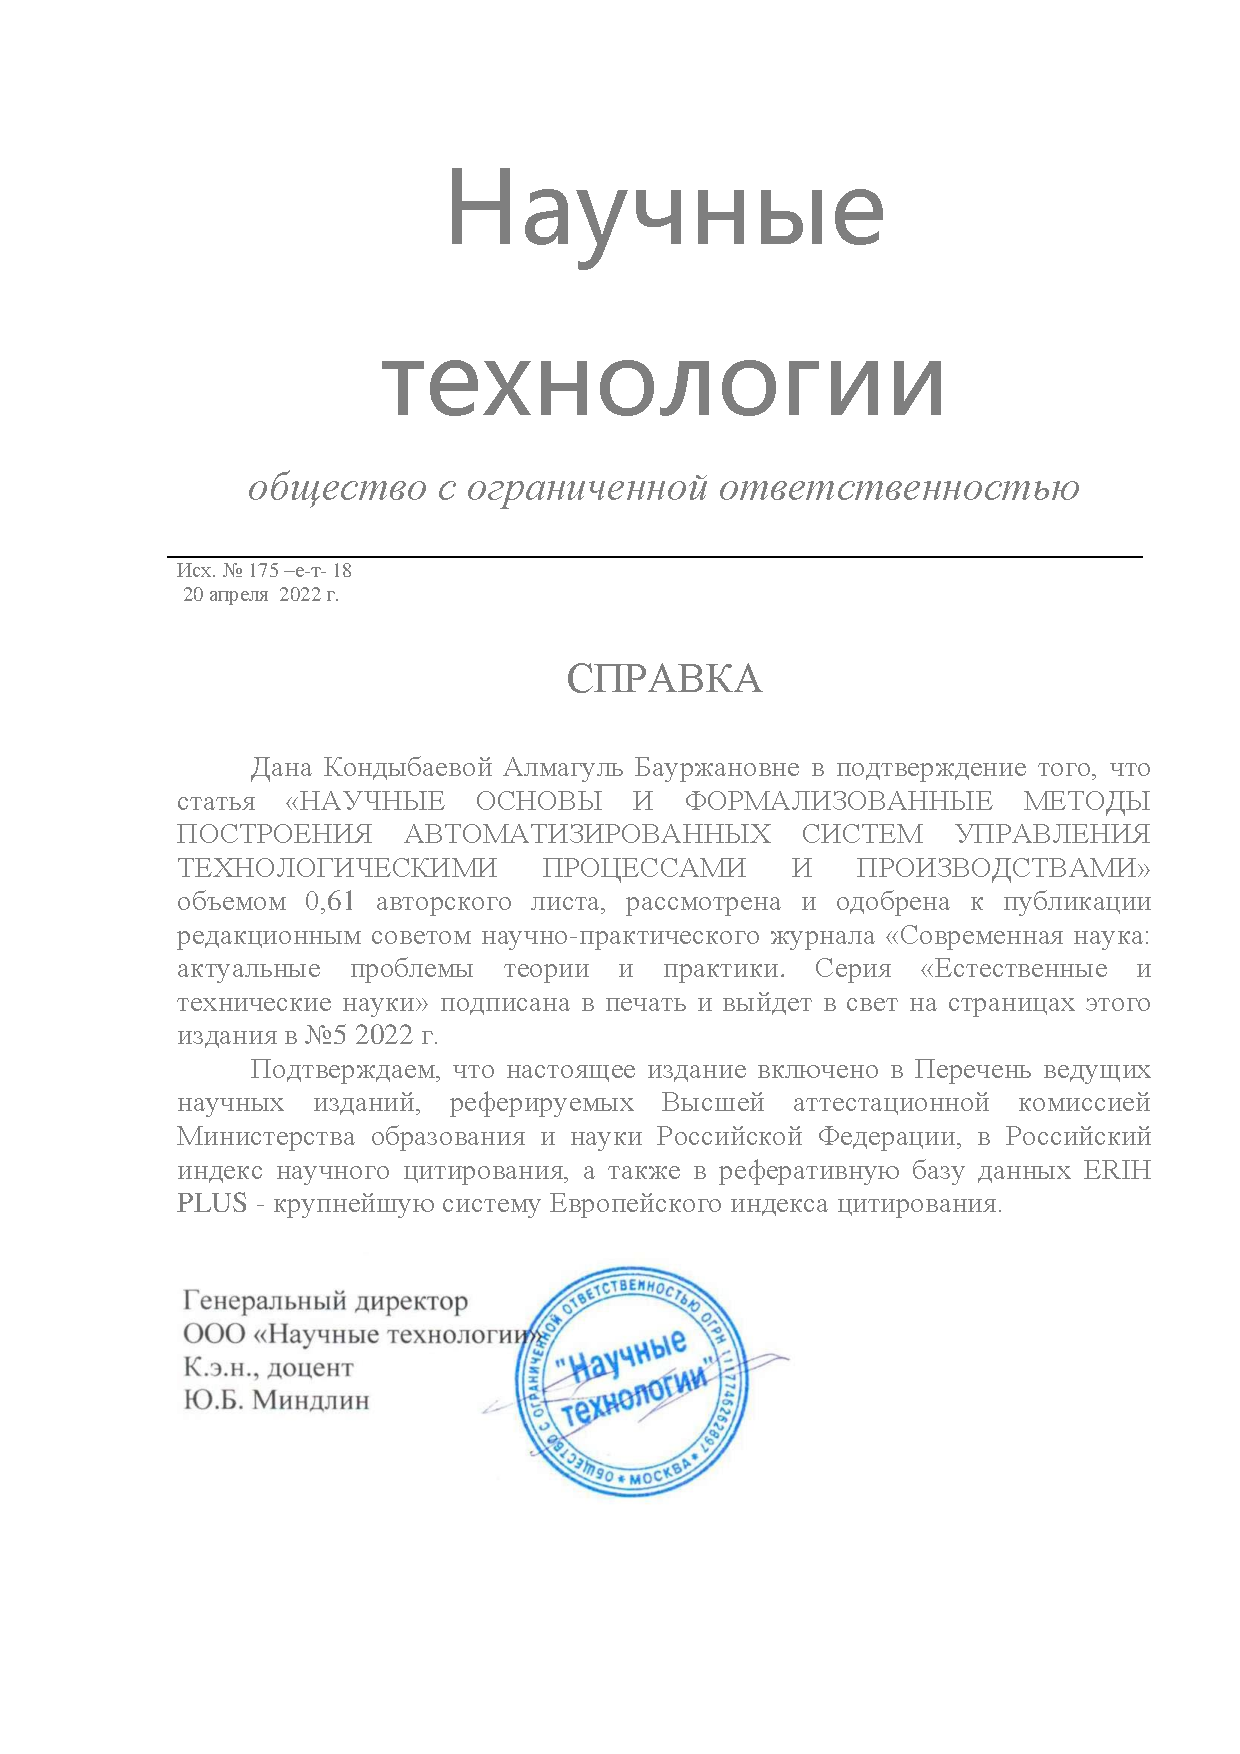
\includepdf[pages=-]{Dissertation/images/drawing.pdf}

\addcontentsline{toc}{appendix}{\protect\chapternumberline{\thechapter}Справка №2 о публикации ВАК}
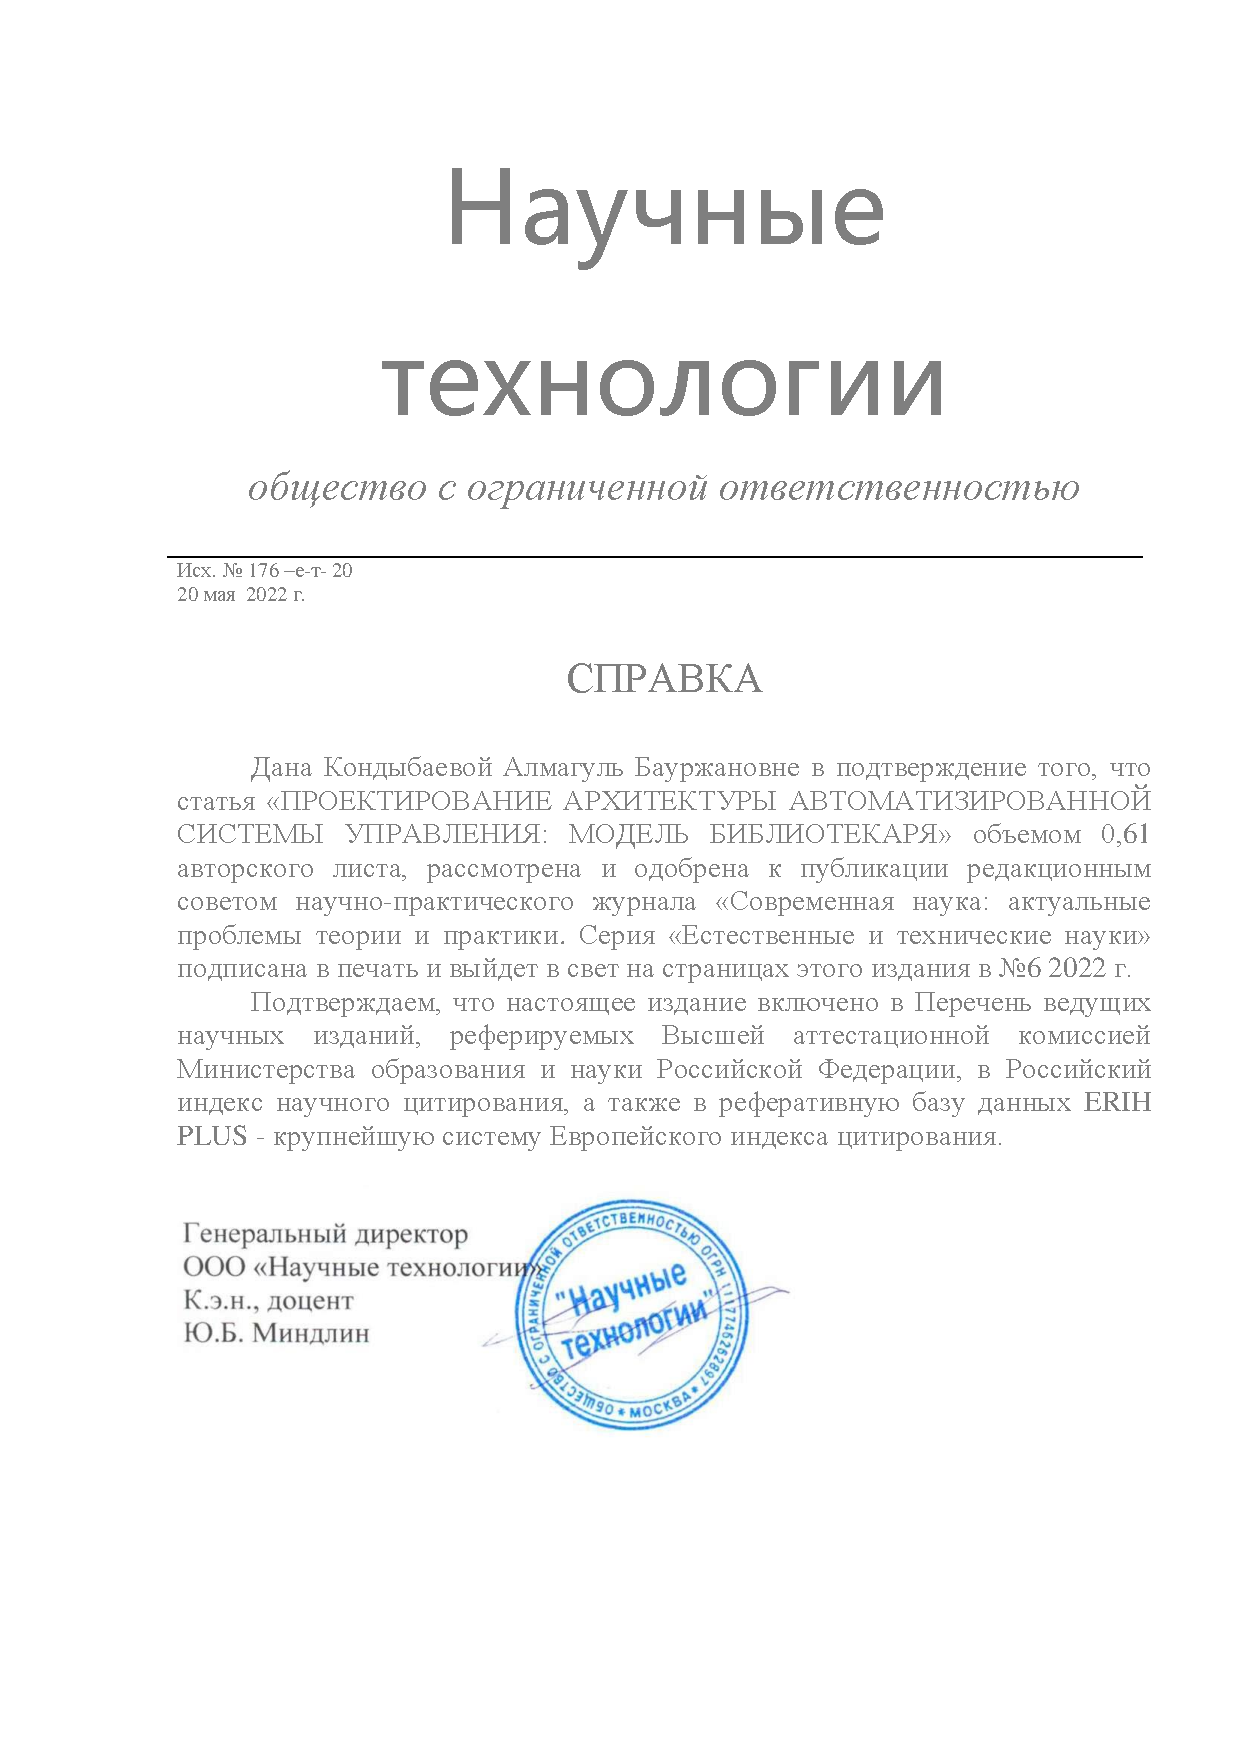
\includepdf[pages=-]{Dissertation/images/drawing1.pdf}
\addcontentsline{toc}{appendix}{\protect\chapternumberline{\thechapter}Статья опубликована в журнале из перечня ВАК}
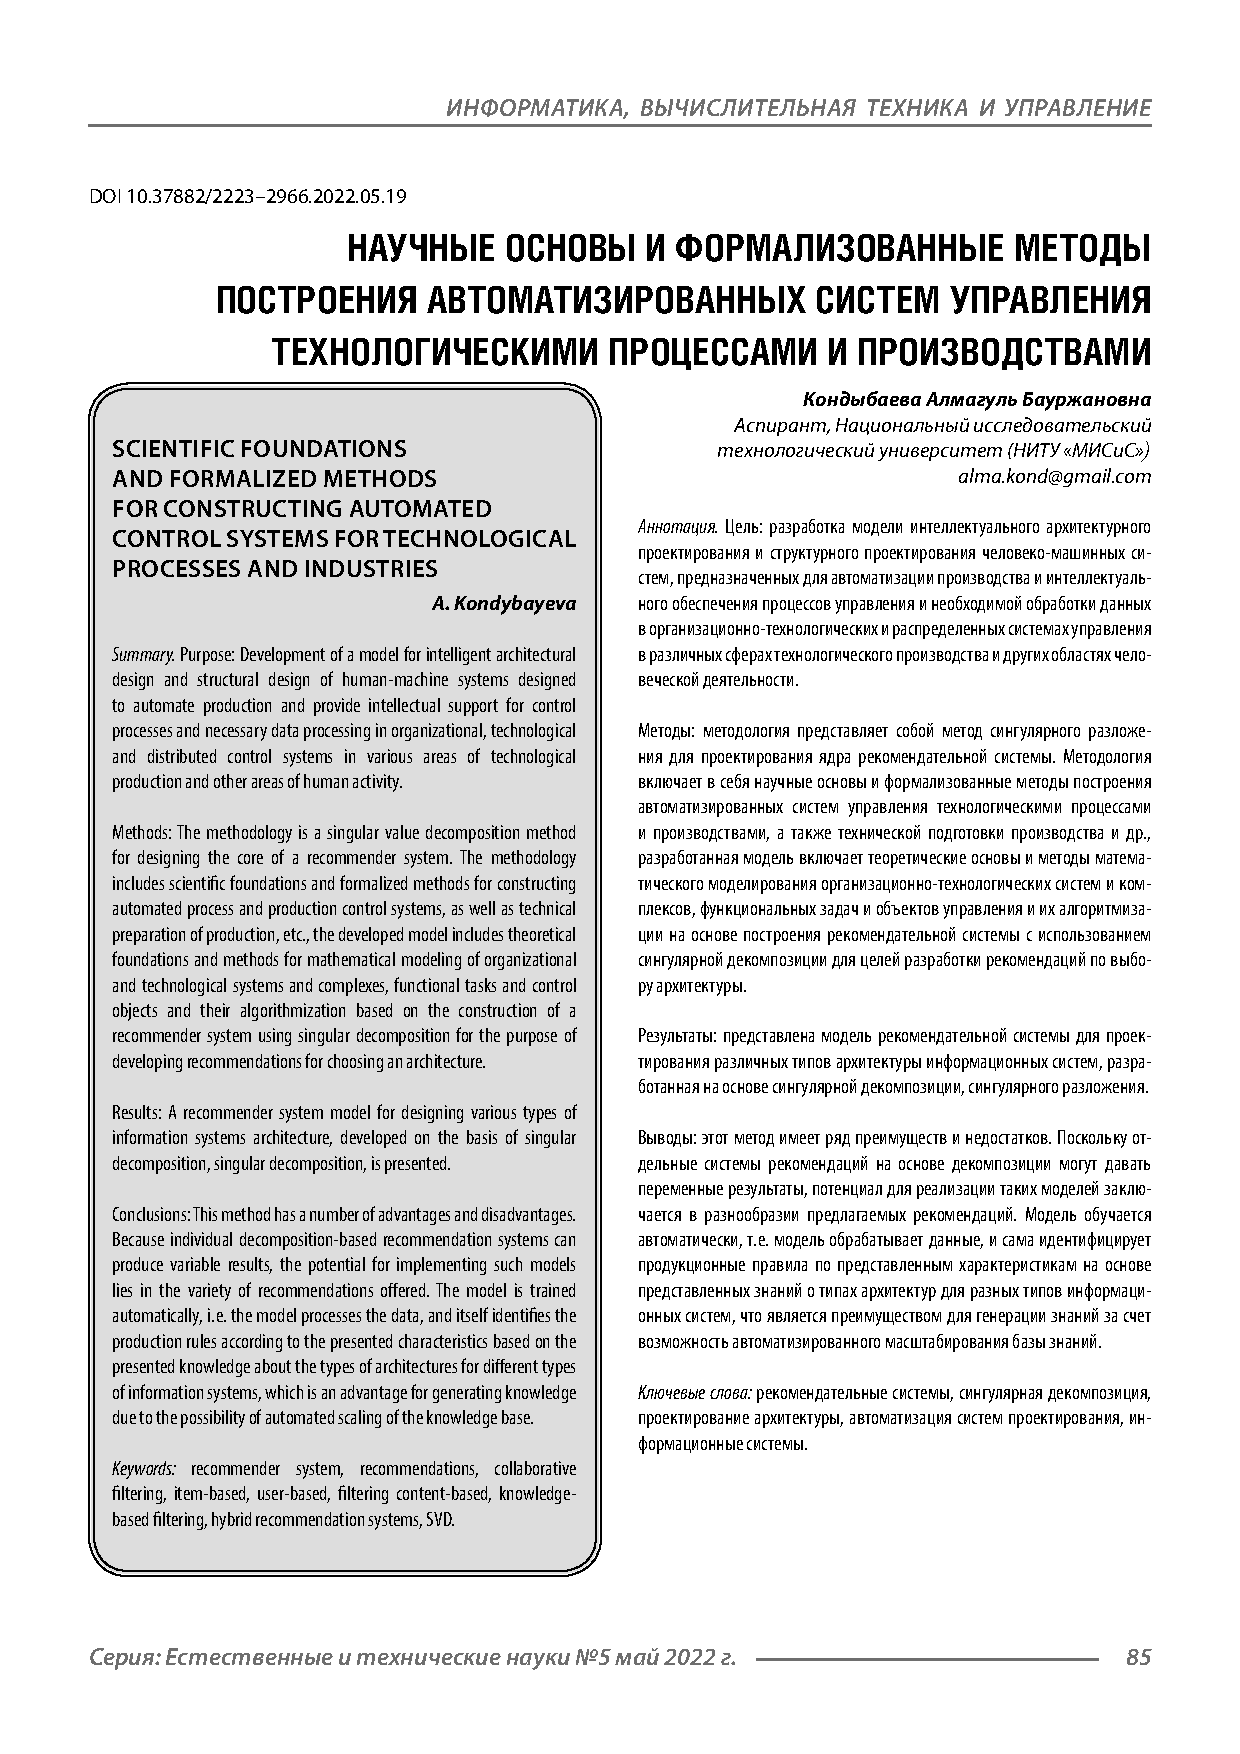
\includepdf[pages=-]{Dissertation/images/p15.pdf}

\addcontentsline{toc}{appendix}{\protect\chapternumberline{\thechapter}Статья опубликована в журнале из перечня ВАК}
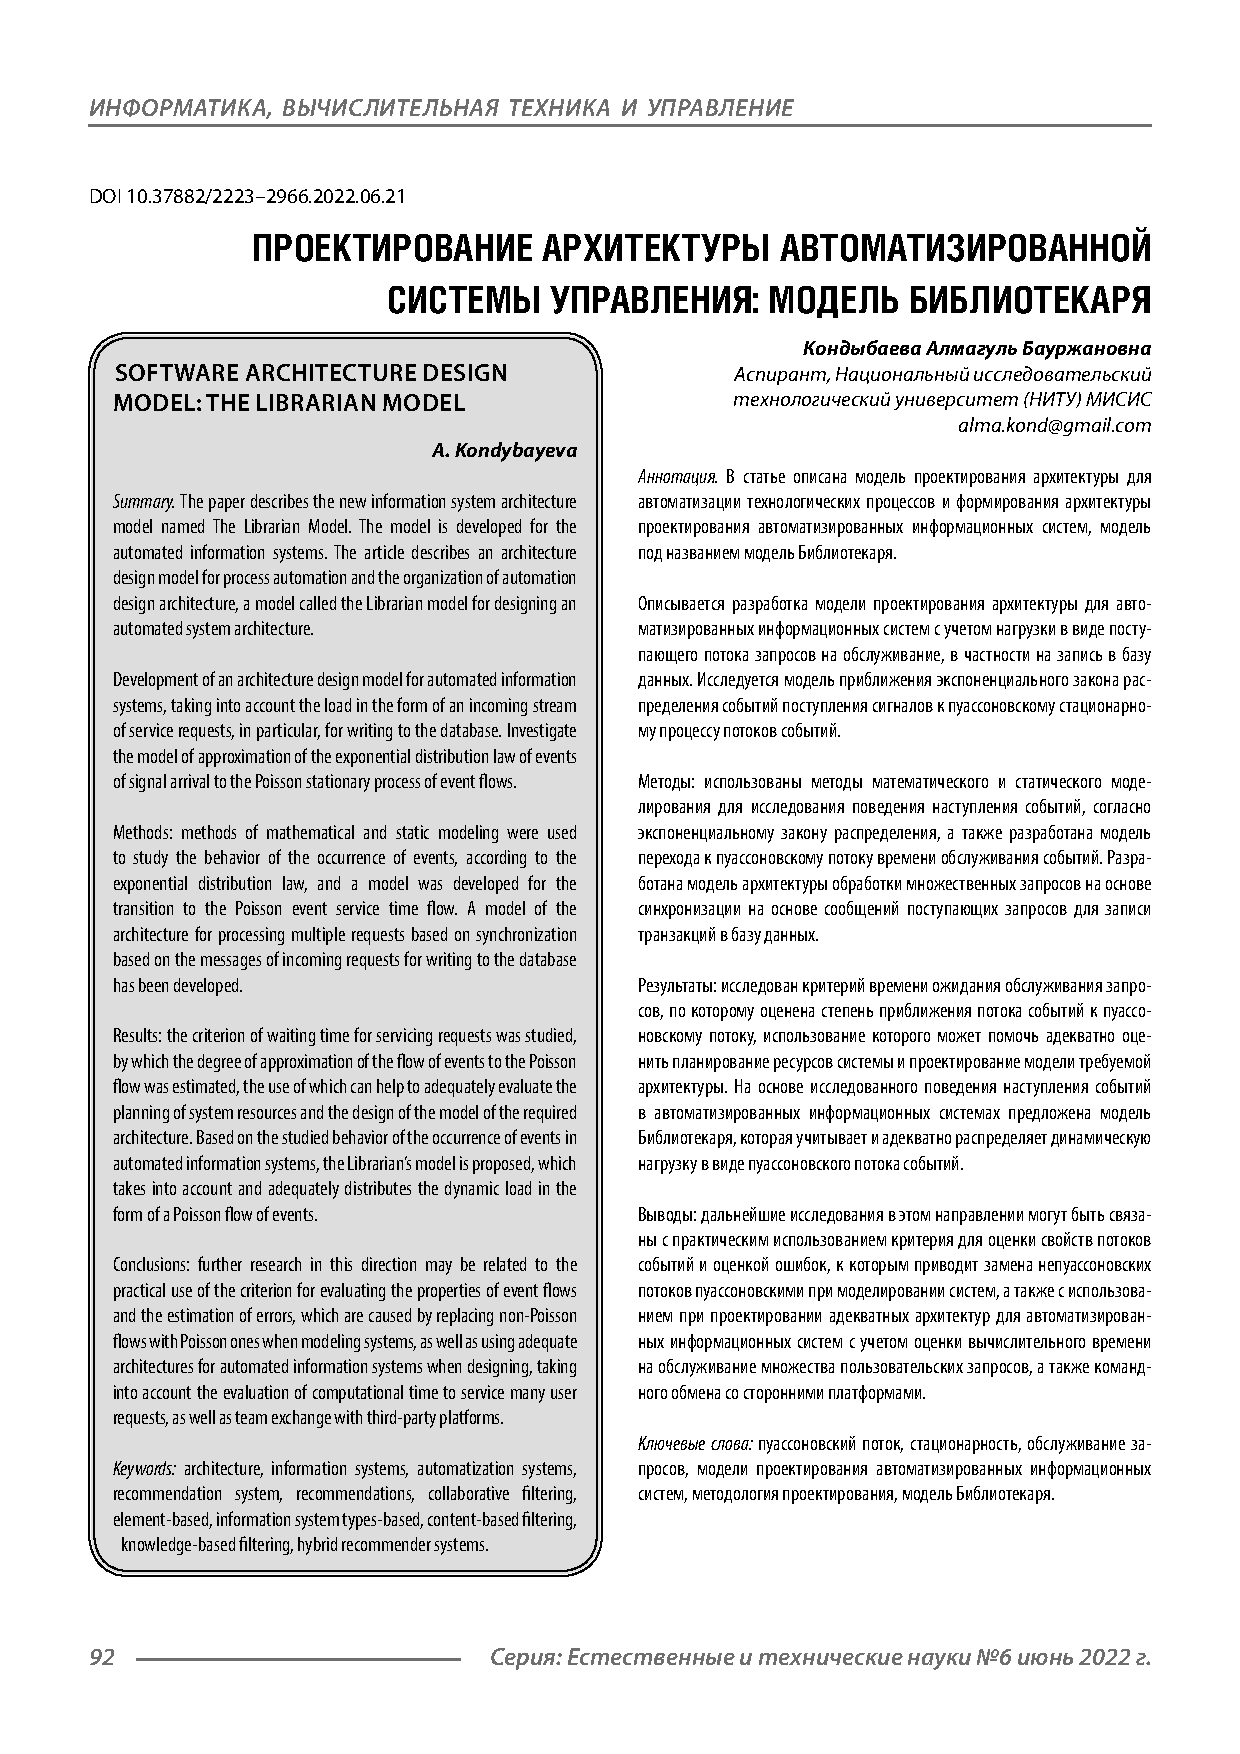
\includepdf[pages=-]{Dissertation/images/p16.pdf}


\section{Справки о внедрении}\label{app:B4}
\clearpage
\refstepcounter{chapter}
\addcontentsline{toc}{appendix}{\protect\chapternumberline{\thechapter}Справки о внедрении}
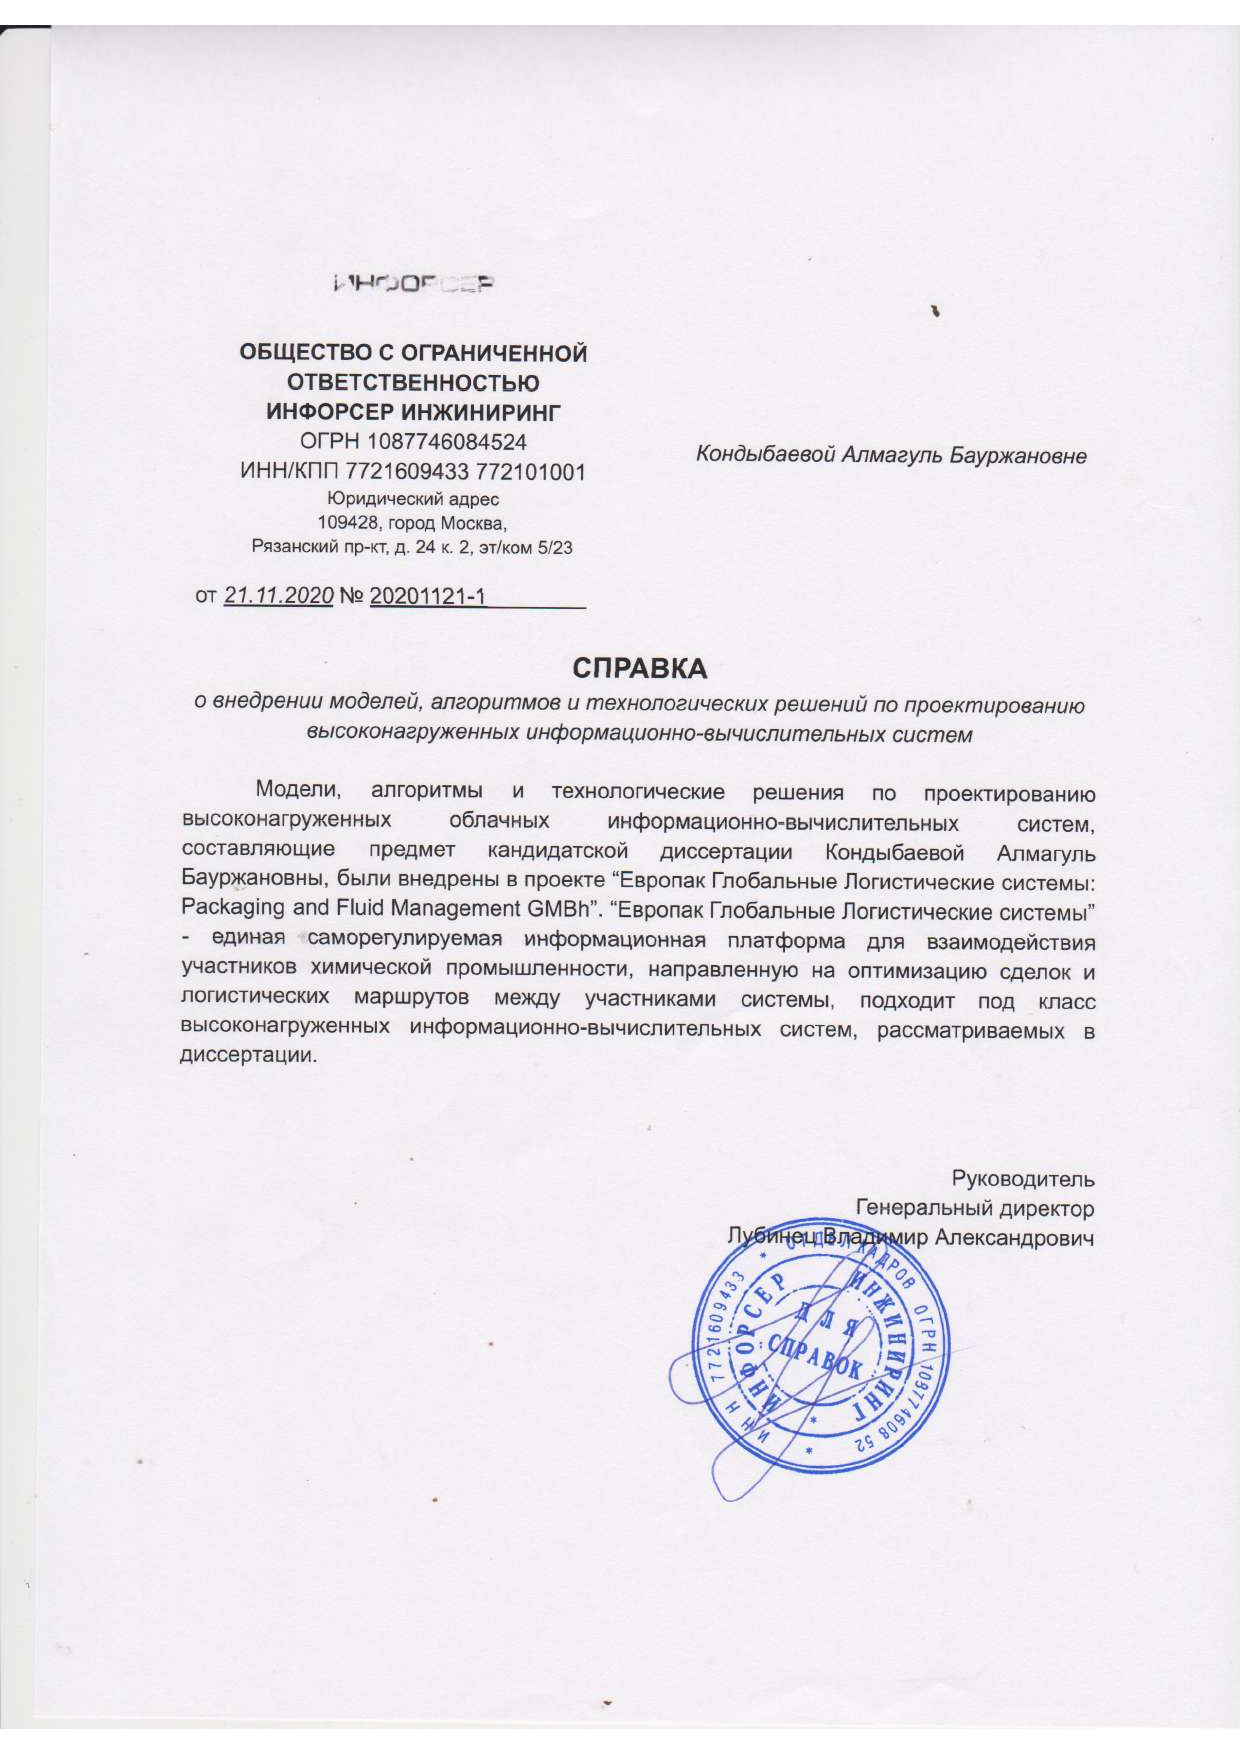
\includepdf[pages=-]{Dissertation/images/drawing2.pdf}


        % Приложения

\setcounter{totalappendix}{\value{chapter}} % Подсчёт количества приложений

\end{document}
